\documentclass[twoside]{book}

% Packages required by doxygen
\usepackage{fixltx2e}
\usepackage{calc}
\usepackage{doxygen}
\usepackage{graphicx}
\usepackage[utf8]{inputenc}
\usepackage{makeidx}
\usepackage{multicol}
\usepackage{multirow}
\PassOptionsToPackage{warn}{textcomp}
\usepackage{textcomp}
\usepackage[nointegrals]{wasysym}
\usepackage[table]{xcolor}

% Font selection
\usepackage[T1]{fontenc}
\usepackage{mathptmx}
\usepackage[scaled=.90]{helvet}
\usepackage{courier}
\usepackage{amssymb}
\usepackage{sectsty}
\renewcommand{\familydefault}{\sfdefault}
\allsectionsfont{%
  \fontseries{bc}\selectfont%
  \color{darkgray}%
}
\renewcommand{\DoxyLabelFont}{%
  \fontseries{bc}\selectfont%
  \color{darkgray}%
}
\newcommand{\+}{\discretionary{\mbox{\scriptsize$\hookleftarrow$}}{}{}}

% Page & text layout
\usepackage{geometry}
\geometry{%
  a4paper,%
  top=2.5cm,%
  bottom=2.5cm,%
  left=2.5cm,%
  right=2.5cm%
}
\tolerance=750
\hfuzz=15pt
\hbadness=750
\setlength{\emergencystretch}{15pt}
\setlength{\parindent}{0cm}
\setlength{\parskip}{0.2cm}
\makeatletter
\renewcommand{\paragraph}{%
  \@startsection{paragraph}{4}{0ex}{-1.0ex}{1.0ex}{%
    \normalfont\normalsize\bfseries\SS@parafont%
  }%
}
\renewcommand{\subparagraph}{%
  \@startsection{subparagraph}{5}{0ex}{-1.0ex}{1.0ex}{%
    \normalfont\normalsize\bfseries\SS@subparafont%
  }%
}
\makeatother

% Headers & footers
\usepackage{fancyhdr}
\pagestyle{fancyplain}
\fancyhead[LE]{\fancyplain{}{\bfseries\thepage}}
\fancyhead[CE]{\fancyplain{}{}}
\fancyhead[RE]{\fancyplain{}{\bfseries\leftmark}}
\fancyhead[LO]{\fancyplain{}{\bfseries\rightmark}}
\fancyhead[CO]{\fancyplain{}{}}
\fancyhead[RO]{\fancyplain{}{\bfseries\thepage}}
\fancyfoot[LE]{\fancyplain{}{}}
\fancyfoot[CE]{\fancyplain{}{}}
\fancyfoot[RE]{\fancyplain{}{\bfseries\scriptsize Generated on Sat Apr 23 2016 11\+:45\+:39 for Inode by Doxygen }}
\fancyfoot[LO]{\fancyplain{}{\bfseries\scriptsize Generated on Sat Apr 23 2016 11\+:45\+:39 for Inode by Doxygen }}
\fancyfoot[CO]{\fancyplain{}{}}
\fancyfoot[RO]{\fancyplain{}{}}
\renewcommand{\footrulewidth}{0.4pt}
\renewcommand{\chaptermark}[1]{%
  \markboth{#1}{}%
}
\renewcommand{\sectionmark}[1]{%
  \markright{\thesection\ #1}%
}

% Indices & bibliography
\usepackage{natbib}
\usepackage[titles]{tocloft}
\setcounter{tocdepth}{3}
\setcounter{secnumdepth}{5}
\makeindex

% Hyperlinks (required, but should be loaded last)
\usepackage{ifpdf}
\ifpdf
  \usepackage[pdftex,pagebackref=true]{hyperref}
\else
  \usepackage[ps2pdf,pagebackref=true]{hyperref}
\fi
\hypersetup{%
  colorlinks=true,%
  linkcolor=blue,%
  citecolor=blue,%
  unicode%
}

% Custom commands
\newcommand{\clearemptydoublepage}{%
  \newpage{\pagestyle{empty}\cleardoublepage}%
}


%===== C O N T E N T S =====

\begin{document}

% Titlepage & ToC
\hypersetup{pageanchor=false,
             bookmarks=true,
             bookmarksnumbered=true,
             pdfencoding=unicode
            }
\pagenumbering{roman}
\begin{titlepage}
\vspace*{7cm}
\begin{center}%
{\Large Inode }\\
\vspace*{1cm}
{\large Generated by Doxygen 1.8.7}\\
\vspace*{0.5cm}
{\small Sat Apr 23 2016 11:45:39}\\
\end{center}
\end{titlepage}
\clearemptydoublepage
\tableofcontents
\clearemptydoublepage
\pagenumbering{arabic}
\hypersetup{pageanchor=true}

%--- Begin generated contents ---
\chapter{Class Index}
\section{Class List}
Here are the classes, structs, unions and interfaces with brief descriptions\+:\begin{DoxyCompactList}
\item\contentsline{section}{\hyperlink{structCmd__t}{Cmd\+\_\+t} }{\pageref{structCmd__t}}{}
\item\contentsline{section}{\hyperlink{structCommand__t}{Command\+\_\+t} }{\pageref{structCommand__t}}{}
\end{DoxyCompactList}

\chapter{File Index}
\section{File List}
Here is a list of all files with brief descriptions\+:\begin{DoxyCompactList}
\item\contentsline{section}{\hyperlink{make_8h}{make.\+h} }{\pageref{make_8h}}{}
\item\contentsline{section}{inc/\hyperlink{inodecli_8h}{inodecli.\+h} }{\pageref{inodecli_8h}}{}
\item\contentsline{section}{inc/\hyperlink{inodedef_8h}{inodedef.\+h} }{\pageref{inodedef_8h}}{}
\item\contentsline{section}{inc/\hyperlink{inodeglob_8h}{inodeglob.\+h} }{\pageref{inodeglob_8h}}{}
\item\contentsline{section}{inc/\hyperlink{inodeinc_8h}{inodeinc.\+h} }{\pageref{inodeinc_8h}}{}
\item\contentsline{section}{inc/\hyperlink{inodeproto_8h}{inodeproto.\+h} }{\pageref{inodeproto_8h}}{}
\item\contentsline{section}{inc/\hyperlink{inodetdfs_8h}{inodetdfs.\+h} }{\pageref{inodetdfs_8h}}{}
\item\contentsline{section}{inc/\hyperlink{inodetime_8h}{inodetime.\+h} }{\pageref{inodetime_8h}}{}
\item\contentsline{section}{src/\hyperlink{inodecli_8c}{inodecli.\+c} }{\pageref{inodecli_8c}}{}
\item\contentsline{section}{src/\hyperlink{inodecmd_8c}{inodecmd.\+c} }{\pageref{inodecmd_8c}}{}
\item\contentsline{section}{src/\hyperlink{inodedir_8c}{inodedir.\+c} }{\pageref{inodedir_8c}}{}
\item\contentsline{section}{src/\hyperlink{inodefix_8c}{inodefix.\+c} }{\pageref{inodefix_8c}}{}
\item\contentsline{section}{src/\hyperlink{inodeinit_8c}{inodeinit.\+c} }{\pageref{inodeinit_8c}}{}
\item\contentsline{section}{src/\hyperlink{inodemain_8c}{inodemain.\+c} }{\pageref{inodemain_8c}}{}
\item\contentsline{section}{src/\hyperlink{inodeutil_8c}{inodeutil.\+c} }{\pageref{inodeutil_8c}}{}
\end{DoxyCompactList}

\chapter{Class Documentation}
\hypertarget{structCmd__t}{\section{Cmd\+\_\+t Struct Reference}
\label{structCmd__t}\index{Cmd\+\_\+t@{Cmd\+\_\+t}}
}


{\ttfamily \#include $<$inodecli.\+h$>$}

\subsection*{Public Attributes}
\begin{DoxyCompactItemize}
\item 
const C\+H\+A\+R $\ast$ \hyperlink{structCmd__t_a3b98f5507e3c73782d6e643f34bd292d}{Name}
\item 
const C\+H\+A\+R $\ast$ \hyperlink{structCmd__t_a9508ec9ed99c99ccd34e3095c463e022}{Help\+Str}
\end{DoxyCompactItemize}


\subsection{Member Data Documentation}
\hypertarget{structCmd__t_a9508ec9ed99c99ccd34e3095c463e022}{\index{Cmd\+\_\+t@{Cmd\+\_\+t}!Help\+Str@{Help\+Str}}
\index{Help\+Str@{Help\+Str}!Cmd\+\_\+t@{Cmd\+\_\+t}}
\subsubsection[{Help\+Str}]{\setlength{\rightskip}{0pt plus 5cm}const C\+H\+A\+R$\ast$ Cmd\+\_\+t\+::\+Help\+Str}}\label{structCmd__t_a9508ec9ed99c99ccd34e3095c463e022}
\hypertarget{structCmd__t_a3b98f5507e3c73782d6e643f34bd292d}{\index{Cmd\+\_\+t@{Cmd\+\_\+t}!Name@{Name}}
\index{Name@{Name}!Cmd\+\_\+t@{Cmd\+\_\+t}}
\subsubsection[{Name}]{\setlength{\rightskip}{0pt plus 5cm}const C\+H\+A\+R$\ast$ Cmd\+\_\+t\+::\+Name}}\label{structCmd__t_a3b98f5507e3c73782d6e643f34bd292d}


The documentation for this struct was generated from the following file\+:\begin{DoxyCompactItemize}
\item 
inc/\hyperlink{inodecli_8h}{inodecli.\+h}\end{DoxyCompactItemize}

\hypertarget{structCommand__t}{\section{Command\+\_\+t Struct Reference}
\label{structCommand__t}\index{Command\+\_\+t@{Command\+\_\+t}}
}


{\ttfamily \#include $<$inodecli.\+h$>$}

\subsection*{Public Attributes}
\begin{DoxyCompactItemize}
\item 
C\+H\+A\+R \hyperlink{structCommand__t_a78320e9f061009774a25879ff29727b7}{Command} \mbox{[}10\mbox{]}
\item 
U\+I\+N\+T4 \hyperlink{structCommand__t_aeadb3c458b96a4a0622e5093eea58f54}{u4\+Cmd\+Id}
\item 
C\+H\+A\+R \hyperlink{structCommand__t_a7a930bcd047b7ed2d5fe372cb9400003}{Options} \mbox{[}5\mbox{]}
\item 
C\+H\+A\+R \hyperlink{structCommand__t_a6f5c12b905882fb8c3e75001895fdba8}{Arg} \mbox{[}100\mbox{]}
\item 
U\+I\+N\+T4 \hyperlink{structCommand__t_aaef7e79094d7a357b0dc8db61e7d4e3b}{u4\+Get\+Id}
\end{DoxyCompactItemize}


\subsection{Member Data Documentation}
\hypertarget{structCommand__t_a6f5c12b905882fb8c3e75001895fdba8}{\index{Command\+\_\+t@{Command\+\_\+t}!Arg@{Arg}}
\index{Arg@{Arg}!Command\+\_\+t@{Command\+\_\+t}}
\subsubsection[{Arg}]{\setlength{\rightskip}{0pt plus 5cm}C\+H\+A\+R Command\+\_\+t\+::\+Arg\mbox{[}100\mbox{]}}}\label{structCommand__t_a6f5c12b905882fb8c3e75001895fdba8}
\hypertarget{structCommand__t_a78320e9f061009774a25879ff29727b7}{\index{Command\+\_\+t@{Command\+\_\+t}!Command@{Command}}
\index{Command@{Command}!Command\+\_\+t@{Command\+\_\+t}}
\subsubsection[{Command}]{\setlength{\rightskip}{0pt plus 5cm}C\+H\+A\+R Command\+\_\+t\+::\+Command\mbox{[}10\mbox{]}}}\label{structCommand__t_a78320e9f061009774a25879ff29727b7}
\hypertarget{structCommand__t_a7a930bcd047b7ed2d5fe372cb9400003}{\index{Command\+\_\+t@{Command\+\_\+t}!Options@{Options}}
\index{Options@{Options}!Command\+\_\+t@{Command\+\_\+t}}
\subsubsection[{Options}]{\setlength{\rightskip}{0pt plus 5cm}C\+H\+A\+R Command\+\_\+t\+::\+Options\mbox{[}5\mbox{]}}}\label{structCommand__t_a7a930bcd047b7ed2d5fe372cb9400003}
\hypertarget{structCommand__t_aeadb3c458b96a4a0622e5093eea58f54}{\index{Command\+\_\+t@{Command\+\_\+t}!u4\+Cmd\+Id@{u4\+Cmd\+Id}}
\index{u4\+Cmd\+Id@{u4\+Cmd\+Id}!Command\+\_\+t@{Command\+\_\+t}}
\subsubsection[{u4\+Cmd\+Id}]{\setlength{\rightskip}{0pt plus 5cm}U\+I\+N\+T4 Command\+\_\+t\+::u4\+Cmd\+Id}}\label{structCommand__t_aeadb3c458b96a4a0622e5093eea58f54}
\hypertarget{structCommand__t_aaef7e79094d7a357b0dc8db61e7d4e3b}{\index{Command\+\_\+t@{Command\+\_\+t}!u4\+Get\+Id@{u4\+Get\+Id}}
\index{u4\+Get\+Id@{u4\+Get\+Id}!Command\+\_\+t@{Command\+\_\+t}}
\subsubsection[{u4\+Get\+Id}]{\setlength{\rightskip}{0pt plus 5cm}U\+I\+N\+T4 Command\+\_\+t\+::u4\+Get\+Id}}\label{structCommand__t_aaef7e79094d7a357b0dc8db61e7d4e3b}


The documentation for this struct was generated from the following file\+:\begin{DoxyCompactItemize}
\item 
inc/\hyperlink{inodecli_8h}{inodecli.\+h}\end{DoxyCompactItemize}

\chapter{File Documentation}
\hypertarget{inodecli_8h}{\section{inc/inodecli.h File Reference}
\label{inodecli_8h}\index{inc/inodecli.\+h@{inc/inodecli.\+h}}
}
{\ttfamily \#include \char`\"{}readinput.\+h\char`\"{}}\\*
Include dependency graph for inodecli.\+h\+:\nopagebreak
\begin{figure}[H]
\begin{center}
\leavevmode
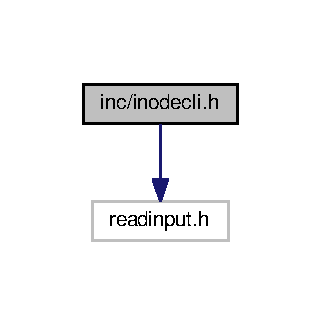
\includegraphics[width=154pt]{inodecli_8h__incl}
\end{center}
\end{figure}
This graph shows which files directly or indirectly include this file\+:\nopagebreak
\begin{figure}[H]
\begin{center}
\leavevmode
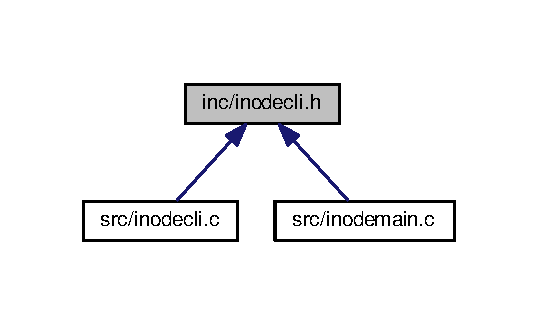
\includegraphics[width=258pt]{inodecli_8h__dep__incl}
\end{center}
\end{figure}
\subsection*{Classes}
\begin{DoxyCompactItemize}
\item 
struct \hyperlink{structCommand__t}{Command\+\_\+t}
\item 
struct \hyperlink{structCmd__t}{Cmd\+\_\+t}
\end{DoxyCompactItemize}
\subsection*{Macros}
\begin{DoxyCompactItemize}
\item 
\#define \hyperlink{inodecli_8h_aac8bef564a684c3ccdf836cfd67a2401}{C\+L\+I\+\_\+\+P\+R\+O\+M\+P\+T}~\char`\"{}Inode Analyser\# \char`\"{}
\item 
\#define \hyperlink{inodecli_8h_a709b8a2a1d68783907c5ab502369e3c9}{C\+M\+D\+\_\+\+D\+E\+L\+I\+M\+I\+T\+E\+R}~\char`\"{} \char`\"{}
\item 
\#define \hyperlink{inodecli_8h_a42553adbbb23a03ca876697c00ea44b1}{C\+M\+D\+\_\+\+H\+E\+L\+P}~\char`\"{}help\char`\"{}
\item 
\#define \hyperlink{inodecli_8h_a4ef842c2bc3e123c98c9379f40a2ab62}{C\+M\+D\+\_\+\+C\+L\+E\+A\+R}~\char`\"{}clear\char`\"{}
\item 
\#define \hyperlink{inodecli_8h_acfa1d482ab47b3ceebb9717007111649}{C\+M\+D\+\_\+\+E\+X\+I\+T}~\char`\"{}exit\char`\"{}
\item 
\#define \hyperlink{inodecli_8h_a7391deb9c3a262ded3e186e94eb884e2}{C\+M\+D\+\_\+\+W\+R\+I\+T\+E}~\char`\"{}write\char`\"{}
\item 
\#define \hyperlink{inodecli_8h_a286bb7f4b865450f58250d939cf45d90}{C\+M\+D\+\_\+\+I\+N\+O\+D\+E}~\char`\"{}inode\char`\"{}
\item 
\#define \hyperlink{inodecli_8h_a9c953a6c538020e644127ee080608021}{C\+M\+D\+\_\+\+R\+E\+A\+D}~\char`\"{}read\char`\"{}
\item 
\#define \hyperlink{inodecli_8h_a3d2223fa832ff3a2aeb97888ce9856f9}{C\+M\+D\+\_\+\+D\+I\+R}~\char`\"{}dir\char`\"{}
\item 
\#define \hyperlink{inodecli_8h_a7517d4f10c0034f27827f5cfe77cf52a}{C\+M\+D\+\_\+\+T\+R\+E\+E}~\char`\"{}tree\char`\"{}
\item 
\#define \hyperlink{inodecli_8h_a430ac043851c4efc20762af91d89f7b9}{C\+M\+D\+\_\+\+C\+O\+R\+R\+U\+P\+T}~\char`\"{}corrupt\char`\"{}
\item 
\#define \hyperlink{inodecli_8h_a68980ecdee8879dfba5618de489ca766}{C\+M\+D\+\_\+\+F\+I\+X}~\char`\"{}fix\char`\"{}
\item 
\#define \hyperlink{inodecli_8h_aebfe91c6148b6492ffab5cdd7ced8b70}{C\+M\+D\+\_\+\+R\+E\+C\+O\+V\+E\+R}~\char`\"{}recover\char`\"{}
\item 
\#define \hyperlink{inodecli_8h_a1b2de4e9466227cd3fcf41b4bf3d74a4}{C\+M\+D\+\_\+\+O\+P\+T\+\_\+\+K\+E\+Y}~\char`\"{}-\/k\char`\"{}
\item 
\#define \hyperlink{inodecli_8h_a35e83bf1e20d880d78af715f43421e8e}{C\+M\+D\+\_\+\+O\+P\+T\+\_\+\+N\+A\+M\+E}~\char`\"{}-\/n\char`\"{}
\item 
\#define \hyperlink{inodecli_8h_a10620eb7066bd16d02eae9ab03365193}{C\+M\+D\+\_\+\+H\+E\+L\+P\+\_\+\+H\+E\+L\+P}~\char`\"{}help -\/ display help\char`\"{}
\item 
\#define \hyperlink{inodecli_8h_ad7afbb455c5f2d60f701118f115080d8}{C\+M\+D\+\_\+\+C\+L\+E\+A\+R\+\_\+\+H\+E\+L\+P}~\char`\"{}clear-\/ clear display\char`\"{}
\item 
\#define \hyperlink{inodecli_8h_a111d2461881013f301a9f648ac24f601}{C\+M\+D\+\_\+\+E\+X\+I\+T\+\_\+\+H\+E\+L\+P}~\char`\"{}exit -\/ exit the application\char`\"{}
\item 
\#define \hyperlink{inodecli_8h_a03adb8dfb4cdd3faba8978163aaf8c93}{C\+M\+D\+\_\+\+R\+E\+A\+D\+\_\+\+H\+E\+L\+P}~\char`\"{}read $<$block number$>$ -\/ display the content of the data block in H\+E\+X\char`\"{}
\item 
\#define \hyperlink{inodecli_8h_a78cd212696a7b049d87aada2a470c965}{C\+M\+D\+\_\+\+W\+R\+I\+T\+E\+\_\+\+H\+E\+L\+P}~\char`\"{}write $<$block number$>$ $<$offset$>$ $<$data$>$ -\/ writes data to a block starting at a particular offset\char`\"{}
\item 
\#define \hyperlink{inodecli_8h_a7b7763747cb82fcd19aa8dd28e30a071}{C\+M\+D\+\_\+\+I\+N\+O\+D\+E\+\_\+\+H\+E\+L\+P}~\char`\"{}inode $<$inode number$>$ -\/ read the inode specified by inode number\char`\"{}
\item 
\#define \hyperlink{inodecli_8h_a5474da458a635be412d5704a02f0df83}{C\+M\+D\+\_\+\+D\+I\+R\+\_\+\+H\+E\+L\+P}~\char`\"{}dir $<$block number$>$ -\/ display the content of the data block of a directory\char`\"{}
\item 
\#define \hyperlink{inodecli_8h_a9008063814b97ecefc54f5a46e19b340}{C\+M\+D\+\_\+\+T\+R\+E\+E\+\_\+\+H\+E\+L\+P}~\char`\"{}tree \mbox{[}inode number\mbox{]} -\/ display the directory tree starting at inode number\char`\"{}
\item 
\#define \hyperlink{inodecli_8h_a57a92b33d047525dc9e69eb72de6269e}{C\+M\+D\+\_\+\+C\+O\+R\+R\+U\+P\+T\+\_\+\+H\+E\+L\+P}~\char`\"{}corrupt $<$inode number$>$ -\/ corrupt the data block pointer of the given inode\char`\"{}
\item 
\#define \hyperlink{inodecli_8h_af2e6404e0cf07b14693e23d54937f010}{C\+M\+D\+\_\+\+F\+I\+X\+\_\+\+H\+E\+L\+P}~\char`\"{}fix $<$inode number$>$ -\/ restore the manually corrupted data block pointer of the given inode\char`\"{}
\item 
\#define \hyperlink{inodecli_8h_ab151080fd3feb4380a5bd65353ce60d5}{C\+M\+D\+\_\+\+R\+E\+C\+O\+V\+E\+R\+\_\+\+H\+E\+L\+P}~\char`\"{}recover -\/ run the recovery algorithm\char`\"{}
\end{DoxyCompactItemize}
\subsection*{Typedefs}
\begin{DoxyCompactItemize}
\item 
typedef struct \hyperlink{structCommand__t}{Command\+\_\+t} \hyperlink{inodecli_8h_a5a66cd47ebf8f625f42d8df880975e95}{t\+Command}
\item 
typedef struct \hyperlink{structCmd__t}{Cmd\+\_\+t} \hyperlink{inodecli_8h_a25509e56046d94d7ebcb24fb035f12c1}{t\+Cmd}
\end{DoxyCompactItemize}
\subsection*{Enumerations}
\begin{DoxyCompactItemize}
\item 
enum \{ \\*
\hyperlink{inodecli_8h_a06fc87d81c62e9abb8790b6e5713c55ba655a173e55e3d70f016a8a466caa20a5}{C\+M\+D\+\_\+\+I\+D\+\_\+\+M\+I\+N}, 
\hyperlink{inodecli_8h_a06fc87d81c62e9abb8790b6e5713c55bae0e5751c184e3060dc7f14f48adbc720}{C\+M\+D\+\_\+\+I\+D\+\_\+\+H\+E\+L\+P} = C\+M\+D\+\_\+\+I\+D\+\_\+\+M\+I\+N, 
\hyperlink{inodecli_8h_a06fc87d81c62e9abb8790b6e5713c55ba0671497d2f9e9bb788033b8e62d75ffe}{C\+M\+D\+\_\+\+I\+D\+\_\+\+C\+L\+E\+A\+R}, 
\hyperlink{inodecli_8h_a06fc87d81c62e9abb8790b6e5713c55baad9add317883fc075dd11eaf694b59a4}{C\+M\+D\+\_\+\+I\+D\+\_\+\+E\+X\+I\+T}, 
\\*
\hyperlink{inodecli_8h_a06fc87d81c62e9abb8790b6e5713c55babbd32dffe3d2152cc470fb20b182ead7}{C\+M\+D\+\_\+\+I\+D\+\_\+\+W\+R\+I\+T\+E}, 
\hyperlink{inodecli_8h_a06fc87d81c62e9abb8790b6e5713c55badf311fdf7ada68a1678ed54aacef711a}{C\+M\+D\+\_\+\+I\+D\+\_\+\+I\+N\+O\+D\+E}, 
\hyperlink{inodecli_8h_a06fc87d81c62e9abb8790b6e5713c55bad9030e4dd23b724da98493899a0f625e}{C\+M\+D\+\_\+\+I\+D\+\_\+\+R\+E\+A\+D}, 
\hyperlink{inodecli_8h_a06fc87d81c62e9abb8790b6e5713c55bae74578f3f060b12a382859c0ae59bbda}{C\+M\+D\+\_\+\+I\+D\+\_\+\+D\+I\+R}, 
\\*
\hyperlink{inodecli_8h_a06fc87d81c62e9abb8790b6e5713c55ba1c16a4c12e7e2cf4aee99df8ea16f810}{C\+M\+D\+\_\+\+I\+D\+\_\+\+T\+R\+E\+E}, 
\hyperlink{inodecli_8h_a06fc87d81c62e9abb8790b6e5713c55badae354f4839e186863d07fe9af4bcfe8}{C\+M\+D\+\_\+\+I\+D\+\_\+\+C\+O\+R\+R\+U\+P\+T}, 
\hyperlink{inodecli_8h_a06fc87d81c62e9abb8790b6e5713c55ba7899d435504c6b1a089a0e04b81df353}{C\+M\+D\+\_\+\+I\+D\+\_\+\+F\+I\+X}, 
\hyperlink{inodecli_8h_a06fc87d81c62e9abb8790b6e5713c55ba801fdb8c23bd8cf52cc4bb3cf0025a84}{C\+M\+D\+\_\+\+I\+D\+\_\+\+R\+E\+C\+O\+V\+E\+R}, 
\\*
\hyperlink{inodecli_8h_a06fc87d81c62e9abb8790b6e5713c55ba0b2e221172240c1b6e6cea012317fb16}{C\+M\+D\+\_\+\+I\+D\+\_\+\+M\+A\+X}, 
\hyperlink{inodecli_8h_a06fc87d81c62e9abb8790b6e5713c55ba20c9a99977545ef5a736321cb199ca2c}{C\+M\+D\+\_\+\+I\+D\+\_\+\+I\+N\+V\+A\+L\+I\+D} = C\+M\+D\+\_\+\+I\+D\+\_\+\+M\+A\+X
 \}
\item 
enum \{ \hyperlink{inodecli_8h_adf764cbdea00d65edcd07bb9953ad2b7ae525cd46a2b490551acdc544cb9cb074}{C\+M\+D\+\_\+\+A\+R\+G\+S\+\_\+0}, 
\hyperlink{inodecli_8h_adf764cbdea00d65edcd07bb9953ad2b7a0eb12d6023709e97ba8ca53bf91a7c24}{C\+M\+D\+\_\+\+A\+R\+G\+S\+\_\+1}, 
\hyperlink{inodecli_8h_adf764cbdea00d65edcd07bb9953ad2b7a26d48e69d8cd13c226f1769208d07a15}{C\+M\+D\+\_\+\+A\+R\+G\+S\+\_\+2}
 \}
\end{DoxyCompactItemize}
\subsection*{Functions}
\begin{DoxyCompactItemize}
\item 
V\+O\+I\+D \hyperlink{inodecli_8h_aa0b53520e1018955fde7aea285159808}{Inode\+Cli\+Start} ()
\item 
V\+O\+I\+D \hyperlink{inodecli_8h_adde588bd205c9ef530fa02ef8f48cf69}{Inode\+Cli\+Handle\+Cmd} (C\+H\+A\+R $\ast$p\+Cmd)
\item 
V\+O\+I\+D \hyperlink{inodecli_8h_a3157714cddf8864e002915be47a6cef5}{Inode\+Cli\+Cmd\+Action} (\hyperlink{inodecli_8h_a5a66cd47ebf8f625f42d8df880975e95}{t\+Command} cmd)
\item 
I\+N\+T1 \hyperlink{inodecli_8h_adaf1a711f6592434c4f1280c0a92fd22}{Inode\+Cli\+Parse\+Cmd} (C\+H\+A\+R $\ast$p\+Cmd\+Str, \hyperlink{inodecli_8h_a5a66cd47ebf8f625f42d8df880975e95}{t\+Command} $\ast$p\+Cmd)
\item 
I\+N\+T1 \hyperlink{inodecli_8h_a7d2b674c246cdf3d17a7d091c5f187f8}{Inode\+Cli\+Validate\+Cmd} (\hyperlink{inodecli_8h_a5a66cd47ebf8f625f42d8df880975e95}{t\+Command} $\ast$p\+Cmd, U\+I\+N\+T1 u1\+Args\+Count)
\item 
V\+O\+I\+D \hyperlink{inodecli_8h_a1635e6bd723f78d1355e30c815348a34}{Inode\+Cmd\+Read\+Handler} (U\+I\+N\+T4 u4\+Block\+No)
\item 
V\+O\+I\+D \hyperlink{inodecli_8h_a1869e2775252da9a36ecca18ce8198d1}{Inode\+Cmd\+Tree\+Handler} (U\+I\+N\+T4 u4\+Inode)
\end{DoxyCompactItemize}


\subsection{Macro Definition Documentation}
\hypertarget{inodecli_8h_aac8bef564a684c3ccdf836cfd67a2401}{\index{inodecli.\+h@{inodecli.\+h}!C\+L\+I\+\_\+\+P\+R\+O\+M\+P\+T@{C\+L\+I\+\_\+\+P\+R\+O\+M\+P\+T}}
\index{C\+L\+I\+\_\+\+P\+R\+O\+M\+P\+T@{C\+L\+I\+\_\+\+P\+R\+O\+M\+P\+T}!inodecli.\+h@{inodecli.\+h}}
\subsubsection[{C\+L\+I\+\_\+\+P\+R\+O\+M\+P\+T}]{\setlength{\rightskip}{0pt plus 5cm}\#define C\+L\+I\+\_\+\+P\+R\+O\+M\+P\+T~\char`\"{}Inode Analyser\# \char`\"{}}}\label{inodecli_8h_aac8bef564a684c3ccdf836cfd67a2401}
\hypertarget{inodecli_8h_a4ef842c2bc3e123c98c9379f40a2ab62}{\index{inodecli.\+h@{inodecli.\+h}!C\+M\+D\+\_\+\+C\+L\+E\+A\+R@{C\+M\+D\+\_\+\+C\+L\+E\+A\+R}}
\index{C\+M\+D\+\_\+\+C\+L\+E\+A\+R@{C\+M\+D\+\_\+\+C\+L\+E\+A\+R}!inodecli.\+h@{inodecli.\+h}}
\subsubsection[{C\+M\+D\+\_\+\+C\+L\+E\+A\+R}]{\setlength{\rightskip}{0pt plus 5cm}\#define C\+M\+D\+\_\+\+C\+L\+E\+A\+R~\char`\"{}clear\char`\"{}}}\label{inodecli_8h_a4ef842c2bc3e123c98c9379f40a2ab62}
\hypertarget{inodecli_8h_ad7afbb455c5f2d60f701118f115080d8}{\index{inodecli.\+h@{inodecli.\+h}!C\+M\+D\+\_\+\+C\+L\+E\+A\+R\+\_\+\+H\+E\+L\+P@{C\+M\+D\+\_\+\+C\+L\+E\+A\+R\+\_\+\+H\+E\+L\+P}}
\index{C\+M\+D\+\_\+\+C\+L\+E\+A\+R\+\_\+\+H\+E\+L\+P@{C\+M\+D\+\_\+\+C\+L\+E\+A\+R\+\_\+\+H\+E\+L\+P}!inodecli.\+h@{inodecli.\+h}}
\subsubsection[{C\+M\+D\+\_\+\+C\+L\+E\+A\+R\+\_\+\+H\+E\+L\+P}]{\setlength{\rightskip}{0pt plus 5cm}\#define C\+M\+D\+\_\+\+C\+L\+E\+A\+R\+\_\+\+H\+E\+L\+P~\char`\"{}clear-\/ clear display\char`\"{}}}\label{inodecli_8h_ad7afbb455c5f2d60f701118f115080d8}
\hypertarget{inodecli_8h_a430ac043851c4efc20762af91d89f7b9}{\index{inodecli.\+h@{inodecli.\+h}!C\+M\+D\+\_\+\+C\+O\+R\+R\+U\+P\+T@{C\+M\+D\+\_\+\+C\+O\+R\+R\+U\+P\+T}}
\index{C\+M\+D\+\_\+\+C\+O\+R\+R\+U\+P\+T@{C\+M\+D\+\_\+\+C\+O\+R\+R\+U\+P\+T}!inodecli.\+h@{inodecli.\+h}}
\subsubsection[{C\+M\+D\+\_\+\+C\+O\+R\+R\+U\+P\+T}]{\setlength{\rightskip}{0pt plus 5cm}\#define C\+M\+D\+\_\+\+C\+O\+R\+R\+U\+P\+T~\char`\"{}corrupt\char`\"{}}}\label{inodecli_8h_a430ac043851c4efc20762af91d89f7b9}
\hypertarget{inodecli_8h_a57a92b33d047525dc9e69eb72de6269e}{\index{inodecli.\+h@{inodecli.\+h}!C\+M\+D\+\_\+\+C\+O\+R\+R\+U\+P\+T\+\_\+\+H\+E\+L\+P@{C\+M\+D\+\_\+\+C\+O\+R\+R\+U\+P\+T\+\_\+\+H\+E\+L\+P}}
\index{C\+M\+D\+\_\+\+C\+O\+R\+R\+U\+P\+T\+\_\+\+H\+E\+L\+P@{C\+M\+D\+\_\+\+C\+O\+R\+R\+U\+P\+T\+\_\+\+H\+E\+L\+P}!inodecli.\+h@{inodecli.\+h}}
\subsubsection[{C\+M\+D\+\_\+\+C\+O\+R\+R\+U\+P\+T\+\_\+\+H\+E\+L\+P}]{\setlength{\rightskip}{0pt plus 5cm}\#define C\+M\+D\+\_\+\+C\+O\+R\+R\+U\+P\+T\+\_\+\+H\+E\+L\+P~\char`\"{}corrupt $<$inode number$>$ -\/ corrupt the data block pointer of the given inode\char`\"{}}}\label{inodecli_8h_a57a92b33d047525dc9e69eb72de6269e}
\hypertarget{inodecli_8h_a709b8a2a1d68783907c5ab502369e3c9}{\index{inodecli.\+h@{inodecli.\+h}!C\+M\+D\+\_\+\+D\+E\+L\+I\+M\+I\+T\+E\+R@{C\+M\+D\+\_\+\+D\+E\+L\+I\+M\+I\+T\+E\+R}}
\index{C\+M\+D\+\_\+\+D\+E\+L\+I\+M\+I\+T\+E\+R@{C\+M\+D\+\_\+\+D\+E\+L\+I\+M\+I\+T\+E\+R}!inodecli.\+h@{inodecli.\+h}}
\subsubsection[{C\+M\+D\+\_\+\+D\+E\+L\+I\+M\+I\+T\+E\+R}]{\setlength{\rightskip}{0pt plus 5cm}\#define C\+M\+D\+\_\+\+D\+E\+L\+I\+M\+I\+T\+E\+R~\char`\"{} \char`\"{}}}\label{inodecli_8h_a709b8a2a1d68783907c5ab502369e3c9}
\hypertarget{inodecli_8h_a3d2223fa832ff3a2aeb97888ce9856f9}{\index{inodecli.\+h@{inodecli.\+h}!C\+M\+D\+\_\+\+D\+I\+R@{C\+M\+D\+\_\+\+D\+I\+R}}
\index{C\+M\+D\+\_\+\+D\+I\+R@{C\+M\+D\+\_\+\+D\+I\+R}!inodecli.\+h@{inodecli.\+h}}
\subsubsection[{C\+M\+D\+\_\+\+D\+I\+R}]{\setlength{\rightskip}{0pt plus 5cm}\#define C\+M\+D\+\_\+\+D\+I\+R~\char`\"{}dir\char`\"{}}}\label{inodecli_8h_a3d2223fa832ff3a2aeb97888ce9856f9}
\hypertarget{inodecli_8h_a5474da458a635be412d5704a02f0df83}{\index{inodecli.\+h@{inodecli.\+h}!C\+M\+D\+\_\+\+D\+I\+R\+\_\+\+H\+E\+L\+P@{C\+M\+D\+\_\+\+D\+I\+R\+\_\+\+H\+E\+L\+P}}
\index{C\+M\+D\+\_\+\+D\+I\+R\+\_\+\+H\+E\+L\+P@{C\+M\+D\+\_\+\+D\+I\+R\+\_\+\+H\+E\+L\+P}!inodecli.\+h@{inodecli.\+h}}
\subsubsection[{C\+M\+D\+\_\+\+D\+I\+R\+\_\+\+H\+E\+L\+P}]{\setlength{\rightskip}{0pt plus 5cm}\#define C\+M\+D\+\_\+\+D\+I\+R\+\_\+\+H\+E\+L\+P~\char`\"{}dir $<$block number$>$ -\/ display the content of the data block of a directory\char`\"{}}}\label{inodecli_8h_a5474da458a635be412d5704a02f0df83}
\hypertarget{inodecli_8h_acfa1d482ab47b3ceebb9717007111649}{\index{inodecli.\+h@{inodecli.\+h}!C\+M\+D\+\_\+\+E\+X\+I\+T@{C\+M\+D\+\_\+\+E\+X\+I\+T}}
\index{C\+M\+D\+\_\+\+E\+X\+I\+T@{C\+M\+D\+\_\+\+E\+X\+I\+T}!inodecli.\+h@{inodecli.\+h}}
\subsubsection[{C\+M\+D\+\_\+\+E\+X\+I\+T}]{\setlength{\rightskip}{0pt plus 5cm}\#define C\+M\+D\+\_\+\+E\+X\+I\+T~\char`\"{}exit\char`\"{}}}\label{inodecli_8h_acfa1d482ab47b3ceebb9717007111649}
\hypertarget{inodecli_8h_a111d2461881013f301a9f648ac24f601}{\index{inodecli.\+h@{inodecli.\+h}!C\+M\+D\+\_\+\+E\+X\+I\+T\+\_\+\+H\+E\+L\+P@{C\+M\+D\+\_\+\+E\+X\+I\+T\+\_\+\+H\+E\+L\+P}}
\index{C\+M\+D\+\_\+\+E\+X\+I\+T\+\_\+\+H\+E\+L\+P@{C\+M\+D\+\_\+\+E\+X\+I\+T\+\_\+\+H\+E\+L\+P}!inodecli.\+h@{inodecli.\+h}}
\subsubsection[{C\+M\+D\+\_\+\+E\+X\+I\+T\+\_\+\+H\+E\+L\+P}]{\setlength{\rightskip}{0pt plus 5cm}\#define C\+M\+D\+\_\+\+E\+X\+I\+T\+\_\+\+H\+E\+L\+P~\char`\"{}exit -\/ exit the application\char`\"{}}}\label{inodecli_8h_a111d2461881013f301a9f648ac24f601}
\hypertarget{inodecli_8h_a68980ecdee8879dfba5618de489ca766}{\index{inodecli.\+h@{inodecli.\+h}!C\+M\+D\+\_\+\+F\+I\+X@{C\+M\+D\+\_\+\+F\+I\+X}}
\index{C\+M\+D\+\_\+\+F\+I\+X@{C\+M\+D\+\_\+\+F\+I\+X}!inodecli.\+h@{inodecli.\+h}}
\subsubsection[{C\+M\+D\+\_\+\+F\+I\+X}]{\setlength{\rightskip}{0pt plus 5cm}\#define C\+M\+D\+\_\+\+F\+I\+X~\char`\"{}fix\char`\"{}}}\label{inodecli_8h_a68980ecdee8879dfba5618de489ca766}
\hypertarget{inodecli_8h_af2e6404e0cf07b14693e23d54937f010}{\index{inodecli.\+h@{inodecli.\+h}!C\+M\+D\+\_\+\+F\+I\+X\+\_\+\+H\+E\+L\+P@{C\+M\+D\+\_\+\+F\+I\+X\+\_\+\+H\+E\+L\+P}}
\index{C\+M\+D\+\_\+\+F\+I\+X\+\_\+\+H\+E\+L\+P@{C\+M\+D\+\_\+\+F\+I\+X\+\_\+\+H\+E\+L\+P}!inodecli.\+h@{inodecli.\+h}}
\subsubsection[{C\+M\+D\+\_\+\+F\+I\+X\+\_\+\+H\+E\+L\+P}]{\setlength{\rightskip}{0pt plus 5cm}\#define C\+M\+D\+\_\+\+F\+I\+X\+\_\+\+H\+E\+L\+P~\char`\"{}fix $<$inode number$>$ -\/ restore the manually corrupted data block pointer of the given inode\char`\"{}}}\label{inodecli_8h_af2e6404e0cf07b14693e23d54937f010}
\hypertarget{inodecli_8h_a42553adbbb23a03ca876697c00ea44b1}{\index{inodecli.\+h@{inodecli.\+h}!C\+M\+D\+\_\+\+H\+E\+L\+P@{C\+M\+D\+\_\+\+H\+E\+L\+P}}
\index{C\+M\+D\+\_\+\+H\+E\+L\+P@{C\+M\+D\+\_\+\+H\+E\+L\+P}!inodecli.\+h@{inodecli.\+h}}
\subsubsection[{C\+M\+D\+\_\+\+H\+E\+L\+P}]{\setlength{\rightskip}{0pt plus 5cm}\#define C\+M\+D\+\_\+\+H\+E\+L\+P~\char`\"{}help\char`\"{}}}\label{inodecli_8h_a42553adbbb23a03ca876697c00ea44b1}
\hypertarget{inodecli_8h_a10620eb7066bd16d02eae9ab03365193}{\index{inodecli.\+h@{inodecli.\+h}!C\+M\+D\+\_\+\+H\+E\+L\+P\+\_\+\+H\+E\+L\+P@{C\+M\+D\+\_\+\+H\+E\+L\+P\+\_\+\+H\+E\+L\+P}}
\index{C\+M\+D\+\_\+\+H\+E\+L\+P\+\_\+\+H\+E\+L\+P@{C\+M\+D\+\_\+\+H\+E\+L\+P\+\_\+\+H\+E\+L\+P}!inodecli.\+h@{inodecli.\+h}}
\subsubsection[{C\+M\+D\+\_\+\+H\+E\+L\+P\+\_\+\+H\+E\+L\+P}]{\setlength{\rightskip}{0pt plus 5cm}\#define C\+M\+D\+\_\+\+H\+E\+L\+P\+\_\+\+H\+E\+L\+P~\char`\"{}help -\/ display help\char`\"{}}}\label{inodecli_8h_a10620eb7066bd16d02eae9ab03365193}
\hypertarget{inodecli_8h_a286bb7f4b865450f58250d939cf45d90}{\index{inodecli.\+h@{inodecli.\+h}!C\+M\+D\+\_\+\+I\+N\+O\+D\+E@{C\+M\+D\+\_\+\+I\+N\+O\+D\+E}}
\index{C\+M\+D\+\_\+\+I\+N\+O\+D\+E@{C\+M\+D\+\_\+\+I\+N\+O\+D\+E}!inodecli.\+h@{inodecli.\+h}}
\subsubsection[{C\+M\+D\+\_\+\+I\+N\+O\+D\+E}]{\setlength{\rightskip}{0pt plus 5cm}\#define C\+M\+D\+\_\+\+I\+N\+O\+D\+E~\char`\"{}inode\char`\"{}}}\label{inodecli_8h_a286bb7f4b865450f58250d939cf45d90}
\hypertarget{inodecli_8h_a7b7763747cb82fcd19aa8dd28e30a071}{\index{inodecli.\+h@{inodecli.\+h}!C\+M\+D\+\_\+\+I\+N\+O\+D\+E\+\_\+\+H\+E\+L\+P@{C\+M\+D\+\_\+\+I\+N\+O\+D\+E\+\_\+\+H\+E\+L\+P}}
\index{C\+M\+D\+\_\+\+I\+N\+O\+D\+E\+\_\+\+H\+E\+L\+P@{C\+M\+D\+\_\+\+I\+N\+O\+D\+E\+\_\+\+H\+E\+L\+P}!inodecli.\+h@{inodecli.\+h}}
\subsubsection[{C\+M\+D\+\_\+\+I\+N\+O\+D\+E\+\_\+\+H\+E\+L\+P}]{\setlength{\rightskip}{0pt plus 5cm}\#define C\+M\+D\+\_\+\+I\+N\+O\+D\+E\+\_\+\+H\+E\+L\+P~\char`\"{}inode $<$inode number$>$ -\/ read the inode specified by inode number\char`\"{}}}\label{inodecli_8h_a7b7763747cb82fcd19aa8dd28e30a071}
\hypertarget{inodecli_8h_a1b2de4e9466227cd3fcf41b4bf3d74a4}{\index{inodecli.\+h@{inodecli.\+h}!C\+M\+D\+\_\+\+O\+P\+T\+\_\+\+K\+E\+Y@{C\+M\+D\+\_\+\+O\+P\+T\+\_\+\+K\+E\+Y}}
\index{C\+M\+D\+\_\+\+O\+P\+T\+\_\+\+K\+E\+Y@{C\+M\+D\+\_\+\+O\+P\+T\+\_\+\+K\+E\+Y}!inodecli.\+h@{inodecli.\+h}}
\subsubsection[{C\+M\+D\+\_\+\+O\+P\+T\+\_\+\+K\+E\+Y}]{\setlength{\rightskip}{0pt plus 5cm}\#define C\+M\+D\+\_\+\+O\+P\+T\+\_\+\+K\+E\+Y~\char`\"{}-\/k\char`\"{}}}\label{inodecli_8h_a1b2de4e9466227cd3fcf41b4bf3d74a4}
\hypertarget{inodecli_8h_a35e83bf1e20d880d78af715f43421e8e}{\index{inodecli.\+h@{inodecli.\+h}!C\+M\+D\+\_\+\+O\+P\+T\+\_\+\+N\+A\+M\+E@{C\+M\+D\+\_\+\+O\+P\+T\+\_\+\+N\+A\+M\+E}}
\index{C\+M\+D\+\_\+\+O\+P\+T\+\_\+\+N\+A\+M\+E@{C\+M\+D\+\_\+\+O\+P\+T\+\_\+\+N\+A\+M\+E}!inodecli.\+h@{inodecli.\+h}}
\subsubsection[{C\+M\+D\+\_\+\+O\+P\+T\+\_\+\+N\+A\+M\+E}]{\setlength{\rightskip}{0pt plus 5cm}\#define C\+M\+D\+\_\+\+O\+P\+T\+\_\+\+N\+A\+M\+E~\char`\"{}-\/n\char`\"{}}}\label{inodecli_8h_a35e83bf1e20d880d78af715f43421e8e}
\hypertarget{inodecli_8h_a9c953a6c538020e644127ee080608021}{\index{inodecli.\+h@{inodecli.\+h}!C\+M\+D\+\_\+\+R\+E\+A\+D@{C\+M\+D\+\_\+\+R\+E\+A\+D}}
\index{C\+M\+D\+\_\+\+R\+E\+A\+D@{C\+M\+D\+\_\+\+R\+E\+A\+D}!inodecli.\+h@{inodecli.\+h}}
\subsubsection[{C\+M\+D\+\_\+\+R\+E\+A\+D}]{\setlength{\rightskip}{0pt plus 5cm}\#define C\+M\+D\+\_\+\+R\+E\+A\+D~\char`\"{}read\char`\"{}}}\label{inodecli_8h_a9c953a6c538020e644127ee080608021}
\hypertarget{inodecli_8h_a03adb8dfb4cdd3faba8978163aaf8c93}{\index{inodecli.\+h@{inodecli.\+h}!C\+M\+D\+\_\+\+R\+E\+A\+D\+\_\+\+H\+E\+L\+P@{C\+M\+D\+\_\+\+R\+E\+A\+D\+\_\+\+H\+E\+L\+P}}
\index{C\+M\+D\+\_\+\+R\+E\+A\+D\+\_\+\+H\+E\+L\+P@{C\+M\+D\+\_\+\+R\+E\+A\+D\+\_\+\+H\+E\+L\+P}!inodecli.\+h@{inodecli.\+h}}
\subsubsection[{C\+M\+D\+\_\+\+R\+E\+A\+D\+\_\+\+H\+E\+L\+P}]{\setlength{\rightskip}{0pt plus 5cm}\#define C\+M\+D\+\_\+\+R\+E\+A\+D\+\_\+\+H\+E\+L\+P~\char`\"{}read $<$block number$>$ -\/ display the content of the data block in H\+E\+X\char`\"{}}}\label{inodecli_8h_a03adb8dfb4cdd3faba8978163aaf8c93}
\hypertarget{inodecli_8h_aebfe91c6148b6492ffab5cdd7ced8b70}{\index{inodecli.\+h@{inodecli.\+h}!C\+M\+D\+\_\+\+R\+E\+C\+O\+V\+E\+R@{C\+M\+D\+\_\+\+R\+E\+C\+O\+V\+E\+R}}
\index{C\+M\+D\+\_\+\+R\+E\+C\+O\+V\+E\+R@{C\+M\+D\+\_\+\+R\+E\+C\+O\+V\+E\+R}!inodecli.\+h@{inodecli.\+h}}
\subsubsection[{C\+M\+D\+\_\+\+R\+E\+C\+O\+V\+E\+R}]{\setlength{\rightskip}{0pt plus 5cm}\#define C\+M\+D\+\_\+\+R\+E\+C\+O\+V\+E\+R~\char`\"{}recover\char`\"{}}}\label{inodecli_8h_aebfe91c6148b6492ffab5cdd7ced8b70}
\hypertarget{inodecli_8h_ab151080fd3feb4380a5bd65353ce60d5}{\index{inodecli.\+h@{inodecli.\+h}!C\+M\+D\+\_\+\+R\+E\+C\+O\+V\+E\+R\+\_\+\+H\+E\+L\+P@{C\+M\+D\+\_\+\+R\+E\+C\+O\+V\+E\+R\+\_\+\+H\+E\+L\+P}}
\index{C\+M\+D\+\_\+\+R\+E\+C\+O\+V\+E\+R\+\_\+\+H\+E\+L\+P@{C\+M\+D\+\_\+\+R\+E\+C\+O\+V\+E\+R\+\_\+\+H\+E\+L\+P}!inodecli.\+h@{inodecli.\+h}}
\subsubsection[{C\+M\+D\+\_\+\+R\+E\+C\+O\+V\+E\+R\+\_\+\+H\+E\+L\+P}]{\setlength{\rightskip}{0pt plus 5cm}\#define C\+M\+D\+\_\+\+R\+E\+C\+O\+V\+E\+R\+\_\+\+H\+E\+L\+P~\char`\"{}recover -\/ run the recovery algorithm\char`\"{}}}\label{inodecli_8h_ab151080fd3feb4380a5bd65353ce60d5}
\hypertarget{inodecli_8h_a7517d4f10c0034f27827f5cfe77cf52a}{\index{inodecli.\+h@{inodecli.\+h}!C\+M\+D\+\_\+\+T\+R\+E\+E@{C\+M\+D\+\_\+\+T\+R\+E\+E}}
\index{C\+M\+D\+\_\+\+T\+R\+E\+E@{C\+M\+D\+\_\+\+T\+R\+E\+E}!inodecli.\+h@{inodecli.\+h}}
\subsubsection[{C\+M\+D\+\_\+\+T\+R\+E\+E}]{\setlength{\rightskip}{0pt plus 5cm}\#define C\+M\+D\+\_\+\+T\+R\+E\+E~\char`\"{}tree\char`\"{}}}\label{inodecli_8h_a7517d4f10c0034f27827f5cfe77cf52a}
\hypertarget{inodecli_8h_a9008063814b97ecefc54f5a46e19b340}{\index{inodecli.\+h@{inodecli.\+h}!C\+M\+D\+\_\+\+T\+R\+E\+E\+\_\+\+H\+E\+L\+P@{C\+M\+D\+\_\+\+T\+R\+E\+E\+\_\+\+H\+E\+L\+P}}
\index{C\+M\+D\+\_\+\+T\+R\+E\+E\+\_\+\+H\+E\+L\+P@{C\+M\+D\+\_\+\+T\+R\+E\+E\+\_\+\+H\+E\+L\+P}!inodecli.\+h@{inodecli.\+h}}
\subsubsection[{C\+M\+D\+\_\+\+T\+R\+E\+E\+\_\+\+H\+E\+L\+P}]{\setlength{\rightskip}{0pt plus 5cm}\#define C\+M\+D\+\_\+\+T\+R\+E\+E\+\_\+\+H\+E\+L\+P~\char`\"{}tree \mbox{[}inode number\mbox{]} -\/ display the directory tree starting at inode number\char`\"{}}}\label{inodecli_8h_a9008063814b97ecefc54f5a46e19b340}
\hypertarget{inodecli_8h_a7391deb9c3a262ded3e186e94eb884e2}{\index{inodecli.\+h@{inodecli.\+h}!C\+M\+D\+\_\+\+W\+R\+I\+T\+E@{C\+M\+D\+\_\+\+W\+R\+I\+T\+E}}
\index{C\+M\+D\+\_\+\+W\+R\+I\+T\+E@{C\+M\+D\+\_\+\+W\+R\+I\+T\+E}!inodecli.\+h@{inodecli.\+h}}
\subsubsection[{C\+M\+D\+\_\+\+W\+R\+I\+T\+E}]{\setlength{\rightskip}{0pt plus 5cm}\#define C\+M\+D\+\_\+\+W\+R\+I\+T\+E~\char`\"{}write\char`\"{}}}\label{inodecli_8h_a7391deb9c3a262ded3e186e94eb884e2}
\hypertarget{inodecli_8h_a78cd212696a7b049d87aada2a470c965}{\index{inodecli.\+h@{inodecli.\+h}!C\+M\+D\+\_\+\+W\+R\+I\+T\+E\+\_\+\+H\+E\+L\+P@{C\+M\+D\+\_\+\+W\+R\+I\+T\+E\+\_\+\+H\+E\+L\+P}}
\index{C\+M\+D\+\_\+\+W\+R\+I\+T\+E\+\_\+\+H\+E\+L\+P@{C\+M\+D\+\_\+\+W\+R\+I\+T\+E\+\_\+\+H\+E\+L\+P}!inodecli.\+h@{inodecli.\+h}}
\subsubsection[{C\+M\+D\+\_\+\+W\+R\+I\+T\+E\+\_\+\+H\+E\+L\+P}]{\setlength{\rightskip}{0pt plus 5cm}\#define C\+M\+D\+\_\+\+W\+R\+I\+T\+E\+\_\+\+H\+E\+L\+P~\char`\"{}write $<$block number$>$ $<$offset$>$ $<$data$>$ -\/ writes data to a block starting at a particular offset\char`\"{}}}\label{inodecli_8h_a78cd212696a7b049d87aada2a470c965}


\subsection{Typedef Documentation}
\hypertarget{inodecli_8h_a25509e56046d94d7ebcb24fb035f12c1}{\index{inodecli.\+h@{inodecli.\+h}!t\+Cmd@{t\+Cmd}}
\index{t\+Cmd@{t\+Cmd}!inodecli.\+h@{inodecli.\+h}}
\subsubsection[{t\+Cmd}]{\setlength{\rightskip}{0pt plus 5cm}typedef struct {\bf Cmd\+\_\+t} {\bf t\+Cmd}}}\label{inodecli_8h_a25509e56046d94d7ebcb24fb035f12c1}
\hypertarget{inodecli_8h_a5a66cd47ebf8f625f42d8df880975e95}{\index{inodecli.\+h@{inodecli.\+h}!t\+Command@{t\+Command}}
\index{t\+Command@{t\+Command}!inodecli.\+h@{inodecli.\+h}}
\subsubsection[{t\+Command}]{\setlength{\rightskip}{0pt plus 5cm}typedef struct {\bf Command\+\_\+t} {\bf t\+Command}}}\label{inodecli_8h_a5a66cd47ebf8f625f42d8df880975e95}


\subsection{Enumeration Type Documentation}
\hypertarget{inodecli_8h_a06fc87d81c62e9abb8790b6e5713c55b}{\subsubsection[{anonymous enum}]{\setlength{\rightskip}{0pt plus 5cm}anonymous enum}}\label{inodecli_8h_a06fc87d81c62e9abb8790b6e5713c55b}
\begin{Desc}
\item[Enumerator]\par
\begin{description}
\index{C\+M\+D\+\_\+\+I\+D\+\_\+\+M\+I\+N@{C\+M\+D\+\_\+\+I\+D\+\_\+\+M\+I\+N}!inodecli.\+h@{inodecli.\+h}}\index{inodecli.\+h@{inodecli.\+h}!C\+M\+D\+\_\+\+I\+D\+\_\+\+M\+I\+N@{C\+M\+D\+\_\+\+I\+D\+\_\+\+M\+I\+N}}\item[{\em 
\hypertarget{inodecli_8h_a06fc87d81c62e9abb8790b6e5713c55ba655a173e55e3d70f016a8a466caa20a5}{C\+M\+D\+\_\+\+I\+D\+\_\+\+M\+I\+N}\label{inodecli_8h_a06fc87d81c62e9abb8790b6e5713c55ba655a173e55e3d70f016a8a466caa20a5}
}]\index{C\+M\+D\+\_\+\+I\+D\+\_\+\+H\+E\+L\+P@{C\+M\+D\+\_\+\+I\+D\+\_\+\+H\+E\+L\+P}!inodecli.\+h@{inodecli.\+h}}\index{inodecli.\+h@{inodecli.\+h}!C\+M\+D\+\_\+\+I\+D\+\_\+\+H\+E\+L\+P@{C\+M\+D\+\_\+\+I\+D\+\_\+\+H\+E\+L\+P}}\item[{\em 
\hypertarget{inodecli_8h_a06fc87d81c62e9abb8790b6e5713c55bae0e5751c184e3060dc7f14f48adbc720}{C\+M\+D\+\_\+\+I\+D\+\_\+\+H\+E\+L\+P}\label{inodecli_8h_a06fc87d81c62e9abb8790b6e5713c55bae0e5751c184e3060dc7f14f48adbc720}
}]\index{C\+M\+D\+\_\+\+I\+D\+\_\+\+C\+L\+E\+A\+R@{C\+M\+D\+\_\+\+I\+D\+\_\+\+C\+L\+E\+A\+R}!inodecli.\+h@{inodecli.\+h}}\index{inodecli.\+h@{inodecli.\+h}!C\+M\+D\+\_\+\+I\+D\+\_\+\+C\+L\+E\+A\+R@{C\+M\+D\+\_\+\+I\+D\+\_\+\+C\+L\+E\+A\+R}}\item[{\em 
\hypertarget{inodecli_8h_a06fc87d81c62e9abb8790b6e5713c55ba0671497d2f9e9bb788033b8e62d75ffe}{C\+M\+D\+\_\+\+I\+D\+\_\+\+C\+L\+E\+A\+R}\label{inodecli_8h_a06fc87d81c62e9abb8790b6e5713c55ba0671497d2f9e9bb788033b8e62d75ffe}
}]\index{C\+M\+D\+\_\+\+I\+D\+\_\+\+E\+X\+I\+T@{C\+M\+D\+\_\+\+I\+D\+\_\+\+E\+X\+I\+T}!inodecli.\+h@{inodecli.\+h}}\index{inodecli.\+h@{inodecli.\+h}!C\+M\+D\+\_\+\+I\+D\+\_\+\+E\+X\+I\+T@{C\+M\+D\+\_\+\+I\+D\+\_\+\+E\+X\+I\+T}}\item[{\em 
\hypertarget{inodecli_8h_a06fc87d81c62e9abb8790b6e5713c55baad9add317883fc075dd11eaf694b59a4}{C\+M\+D\+\_\+\+I\+D\+\_\+\+E\+X\+I\+T}\label{inodecli_8h_a06fc87d81c62e9abb8790b6e5713c55baad9add317883fc075dd11eaf694b59a4}
}]\index{C\+M\+D\+\_\+\+I\+D\+\_\+\+W\+R\+I\+T\+E@{C\+M\+D\+\_\+\+I\+D\+\_\+\+W\+R\+I\+T\+E}!inodecli.\+h@{inodecli.\+h}}\index{inodecli.\+h@{inodecli.\+h}!C\+M\+D\+\_\+\+I\+D\+\_\+\+W\+R\+I\+T\+E@{C\+M\+D\+\_\+\+I\+D\+\_\+\+W\+R\+I\+T\+E}}\item[{\em 
\hypertarget{inodecli_8h_a06fc87d81c62e9abb8790b6e5713c55babbd32dffe3d2152cc470fb20b182ead7}{C\+M\+D\+\_\+\+I\+D\+\_\+\+W\+R\+I\+T\+E}\label{inodecli_8h_a06fc87d81c62e9abb8790b6e5713c55babbd32dffe3d2152cc470fb20b182ead7}
}]\index{C\+M\+D\+\_\+\+I\+D\+\_\+\+I\+N\+O\+D\+E@{C\+M\+D\+\_\+\+I\+D\+\_\+\+I\+N\+O\+D\+E}!inodecli.\+h@{inodecli.\+h}}\index{inodecli.\+h@{inodecli.\+h}!C\+M\+D\+\_\+\+I\+D\+\_\+\+I\+N\+O\+D\+E@{C\+M\+D\+\_\+\+I\+D\+\_\+\+I\+N\+O\+D\+E}}\item[{\em 
\hypertarget{inodecli_8h_a06fc87d81c62e9abb8790b6e5713c55badf311fdf7ada68a1678ed54aacef711a}{C\+M\+D\+\_\+\+I\+D\+\_\+\+I\+N\+O\+D\+E}\label{inodecli_8h_a06fc87d81c62e9abb8790b6e5713c55badf311fdf7ada68a1678ed54aacef711a}
}]\index{C\+M\+D\+\_\+\+I\+D\+\_\+\+R\+E\+A\+D@{C\+M\+D\+\_\+\+I\+D\+\_\+\+R\+E\+A\+D}!inodecli.\+h@{inodecli.\+h}}\index{inodecli.\+h@{inodecli.\+h}!C\+M\+D\+\_\+\+I\+D\+\_\+\+R\+E\+A\+D@{C\+M\+D\+\_\+\+I\+D\+\_\+\+R\+E\+A\+D}}\item[{\em 
\hypertarget{inodecli_8h_a06fc87d81c62e9abb8790b6e5713c55bad9030e4dd23b724da98493899a0f625e}{C\+M\+D\+\_\+\+I\+D\+\_\+\+R\+E\+A\+D}\label{inodecli_8h_a06fc87d81c62e9abb8790b6e5713c55bad9030e4dd23b724da98493899a0f625e}
}]\index{C\+M\+D\+\_\+\+I\+D\+\_\+\+D\+I\+R@{C\+M\+D\+\_\+\+I\+D\+\_\+\+D\+I\+R}!inodecli.\+h@{inodecli.\+h}}\index{inodecli.\+h@{inodecli.\+h}!C\+M\+D\+\_\+\+I\+D\+\_\+\+D\+I\+R@{C\+M\+D\+\_\+\+I\+D\+\_\+\+D\+I\+R}}\item[{\em 
\hypertarget{inodecli_8h_a06fc87d81c62e9abb8790b6e5713c55bae74578f3f060b12a382859c0ae59bbda}{C\+M\+D\+\_\+\+I\+D\+\_\+\+D\+I\+R}\label{inodecli_8h_a06fc87d81c62e9abb8790b6e5713c55bae74578f3f060b12a382859c0ae59bbda}
}]\index{C\+M\+D\+\_\+\+I\+D\+\_\+\+T\+R\+E\+E@{C\+M\+D\+\_\+\+I\+D\+\_\+\+T\+R\+E\+E}!inodecli.\+h@{inodecli.\+h}}\index{inodecli.\+h@{inodecli.\+h}!C\+M\+D\+\_\+\+I\+D\+\_\+\+T\+R\+E\+E@{C\+M\+D\+\_\+\+I\+D\+\_\+\+T\+R\+E\+E}}\item[{\em 
\hypertarget{inodecli_8h_a06fc87d81c62e9abb8790b6e5713c55ba1c16a4c12e7e2cf4aee99df8ea16f810}{C\+M\+D\+\_\+\+I\+D\+\_\+\+T\+R\+E\+E}\label{inodecli_8h_a06fc87d81c62e9abb8790b6e5713c55ba1c16a4c12e7e2cf4aee99df8ea16f810}
}]\index{C\+M\+D\+\_\+\+I\+D\+\_\+\+C\+O\+R\+R\+U\+P\+T@{C\+M\+D\+\_\+\+I\+D\+\_\+\+C\+O\+R\+R\+U\+P\+T}!inodecli.\+h@{inodecli.\+h}}\index{inodecli.\+h@{inodecli.\+h}!C\+M\+D\+\_\+\+I\+D\+\_\+\+C\+O\+R\+R\+U\+P\+T@{C\+M\+D\+\_\+\+I\+D\+\_\+\+C\+O\+R\+R\+U\+P\+T}}\item[{\em 
\hypertarget{inodecli_8h_a06fc87d81c62e9abb8790b6e5713c55badae354f4839e186863d07fe9af4bcfe8}{C\+M\+D\+\_\+\+I\+D\+\_\+\+C\+O\+R\+R\+U\+P\+T}\label{inodecli_8h_a06fc87d81c62e9abb8790b6e5713c55badae354f4839e186863d07fe9af4bcfe8}
}]\index{C\+M\+D\+\_\+\+I\+D\+\_\+\+F\+I\+X@{C\+M\+D\+\_\+\+I\+D\+\_\+\+F\+I\+X}!inodecli.\+h@{inodecli.\+h}}\index{inodecli.\+h@{inodecli.\+h}!C\+M\+D\+\_\+\+I\+D\+\_\+\+F\+I\+X@{C\+M\+D\+\_\+\+I\+D\+\_\+\+F\+I\+X}}\item[{\em 
\hypertarget{inodecli_8h_a06fc87d81c62e9abb8790b6e5713c55ba7899d435504c6b1a089a0e04b81df353}{C\+M\+D\+\_\+\+I\+D\+\_\+\+F\+I\+X}\label{inodecli_8h_a06fc87d81c62e9abb8790b6e5713c55ba7899d435504c6b1a089a0e04b81df353}
}]\index{C\+M\+D\+\_\+\+I\+D\+\_\+\+R\+E\+C\+O\+V\+E\+R@{C\+M\+D\+\_\+\+I\+D\+\_\+\+R\+E\+C\+O\+V\+E\+R}!inodecli.\+h@{inodecli.\+h}}\index{inodecli.\+h@{inodecli.\+h}!C\+M\+D\+\_\+\+I\+D\+\_\+\+R\+E\+C\+O\+V\+E\+R@{C\+M\+D\+\_\+\+I\+D\+\_\+\+R\+E\+C\+O\+V\+E\+R}}\item[{\em 
\hypertarget{inodecli_8h_a06fc87d81c62e9abb8790b6e5713c55ba801fdb8c23bd8cf52cc4bb3cf0025a84}{C\+M\+D\+\_\+\+I\+D\+\_\+\+R\+E\+C\+O\+V\+E\+R}\label{inodecli_8h_a06fc87d81c62e9abb8790b6e5713c55ba801fdb8c23bd8cf52cc4bb3cf0025a84}
}]\index{C\+M\+D\+\_\+\+I\+D\+\_\+\+M\+A\+X@{C\+M\+D\+\_\+\+I\+D\+\_\+\+M\+A\+X}!inodecli.\+h@{inodecli.\+h}}\index{inodecli.\+h@{inodecli.\+h}!C\+M\+D\+\_\+\+I\+D\+\_\+\+M\+A\+X@{C\+M\+D\+\_\+\+I\+D\+\_\+\+M\+A\+X}}\item[{\em 
\hypertarget{inodecli_8h_a06fc87d81c62e9abb8790b6e5713c55ba0b2e221172240c1b6e6cea012317fb16}{C\+M\+D\+\_\+\+I\+D\+\_\+\+M\+A\+X}\label{inodecli_8h_a06fc87d81c62e9abb8790b6e5713c55ba0b2e221172240c1b6e6cea012317fb16}
}]\index{C\+M\+D\+\_\+\+I\+D\+\_\+\+I\+N\+V\+A\+L\+I\+D@{C\+M\+D\+\_\+\+I\+D\+\_\+\+I\+N\+V\+A\+L\+I\+D}!inodecli.\+h@{inodecli.\+h}}\index{inodecli.\+h@{inodecli.\+h}!C\+M\+D\+\_\+\+I\+D\+\_\+\+I\+N\+V\+A\+L\+I\+D@{C\+M\+D\+\_\+\+I\+D\+\_\+\+I\+N\+V\+A\+L\+I\+D}}\item[{\em 
\hypertarget{inodecli_8h_a06fc87d81c62e9abb8790b6e5713c55ba20c9a99977545ef5a736321cb199ca2c}{C\+M\+D\+\_\+\+I\+D\+\_\+\+I\+N\+V\+A\+L\+I\+D}\label{inodecli_8h_a06fc87d81c62e9abb8790b6e5713c55ba20c9a99977545ef5a736321cb199ca2c}
}]\end{description}
\end{Desc}
\hypertarget{inodecli_8h_adf764cbdea00d65edcd07bb9953ad2b7}{\subsubsection[{anonymous enum}]{\setlength{\rightskip}{0pt plus 5cm}anonymous enum}}\label{inodecli_8h_adf764cbdea00d65edcd07bb9953ad2b7}
\begin{Desc}
\item[Enumerator]\par
\begin{description}
\index{C\+M\+D\+\_\+\+A\+R\+G\+S\+\_\+0@{C\+M\+D\+\_\+\+A\+R\+G\+S\+\_\+0}!inodecli.\+h@{inodecli.\+h}}\index{inodecli.\+h@{inodecli.\+h}!C\+M\+D\+\_\+\+A\+R\+G\+S\+\_\+0@{C\+M\+D\+\_\+\+A\+R\+G\+S\+\_\+0}}\item[{\em 
\hypertarget{inodecli_8h_adf764cbdea00d65edcd07bb9953ad2b7ae525cd46a2b490551acdc544cb9cb074}{C\+M\+D\+\_\+\+A\+R\+G\+S\+\_\+0}\label{inodecli_8h_adf764cbdea00d65edcd07bb9953ad2b7ae525cd46a2b490551acdc544cb9cb074}
}]\index{C\+M\+D\+\_\+\+A\+R\+G\+S\+\_\+1@{C\+M\+D\+\_\+\+A\+R\+G\+S\+\_\+1}!inodecli.\+h@{inodecli.\+h}}\index{inodecli.\+h@{inodecli.\+h}!C\+M\+D\+\_\+\+A\+R\+G\+S\+\_\+1@{C\+M\+D\+\_\+\+A\+R\+G\+S\+\_\+1}}\item[{\em 
\hypertarget{inodecli_8h_adf764cbdea00d65edcd07bb9953ad2b7a0eb12d6023709e97ba8ca53bf91a7c24}{C\+M\+D\+\_\+\+A\+R\+G\+S\+\_\+1}\label{inodecli_8h_adf764cbdea00d65edcd07bb9953ad2b7a0eb12d6023709e97ba8ca53bf91a7c24}
}]\index{C\+M\+D\+\_\+\+A\+R\+G\+S\+\_\+2@{C\+M\+D\+\_\+\+A\+R\+G\+S\+\_\+2}!inodecli.\+h@{inodecli.\+h}}\index{inodecli.\+h@{inodecli.\+h}!C\+M\+D\+\_\+\+A\+R\+G\+S\+\_\+2@{C\+M\+D\+\_\+\+A\+R\+G\+S\+\_\+2}}\item[{\em 
\hypertarget{inodecli_8h_adf764cbdea00d65edcd07bb9953ad2b7a26d48e69d8cd13c226f1769208d07a15}{C\+M\+D\+\_\+\+A\+R\+G\+S\+\_\+2}\label{inodecli_8h_adf764cbdea00d65edcd07bb9953ad2b7a26d48e69d8cd13c226f1769208d07a15}
}]\end{description}
\end{Desc}


\subsection{Function Documentation}
\hypertarget{inodecli_8h_a3157714cddf8864e002915be47a6cef5}{\index{inodecli.\+h@{inodecli.\+h}!Inode\+Cli\+Cmd\+Action@{Inode\+Cli\+Cmd\+Action}}
\index{Inode\+Cli\+Cmd\+Action@{Inode\+Cli\+Cmd\+Action}!inodecli.\+h@{inodecli.\+h}}
\subsubsection[{Inode\+Cli\+Cmd\+Action}]{\setlength{\rightskip}{0pt plus 5cm}V\+O\+I\+D Inode\+Cli\+Cmd\+Action (
\begin{DoxyParamCaption}
\item[{{\bf t\+Command}}]{cmd}
\end{DoxyParamCaption}
)}}\label{inodecli_8h_a3157714cddf8864e002915be47a6cef5}


 Function Name \+: Inode\+Cli\+Cmd\+Action

Description \+: This Function is the overall action handler. This function identifies the command and the action to be taken for the command.

Input \+: cmd -\/ structure containing the parsed command and arguments

Output \+: None

Returns \+: None 

Here is the call graph for this function\+:\nopagebreak
\begin{figure}[H]
\begin{center}
\leavevmode
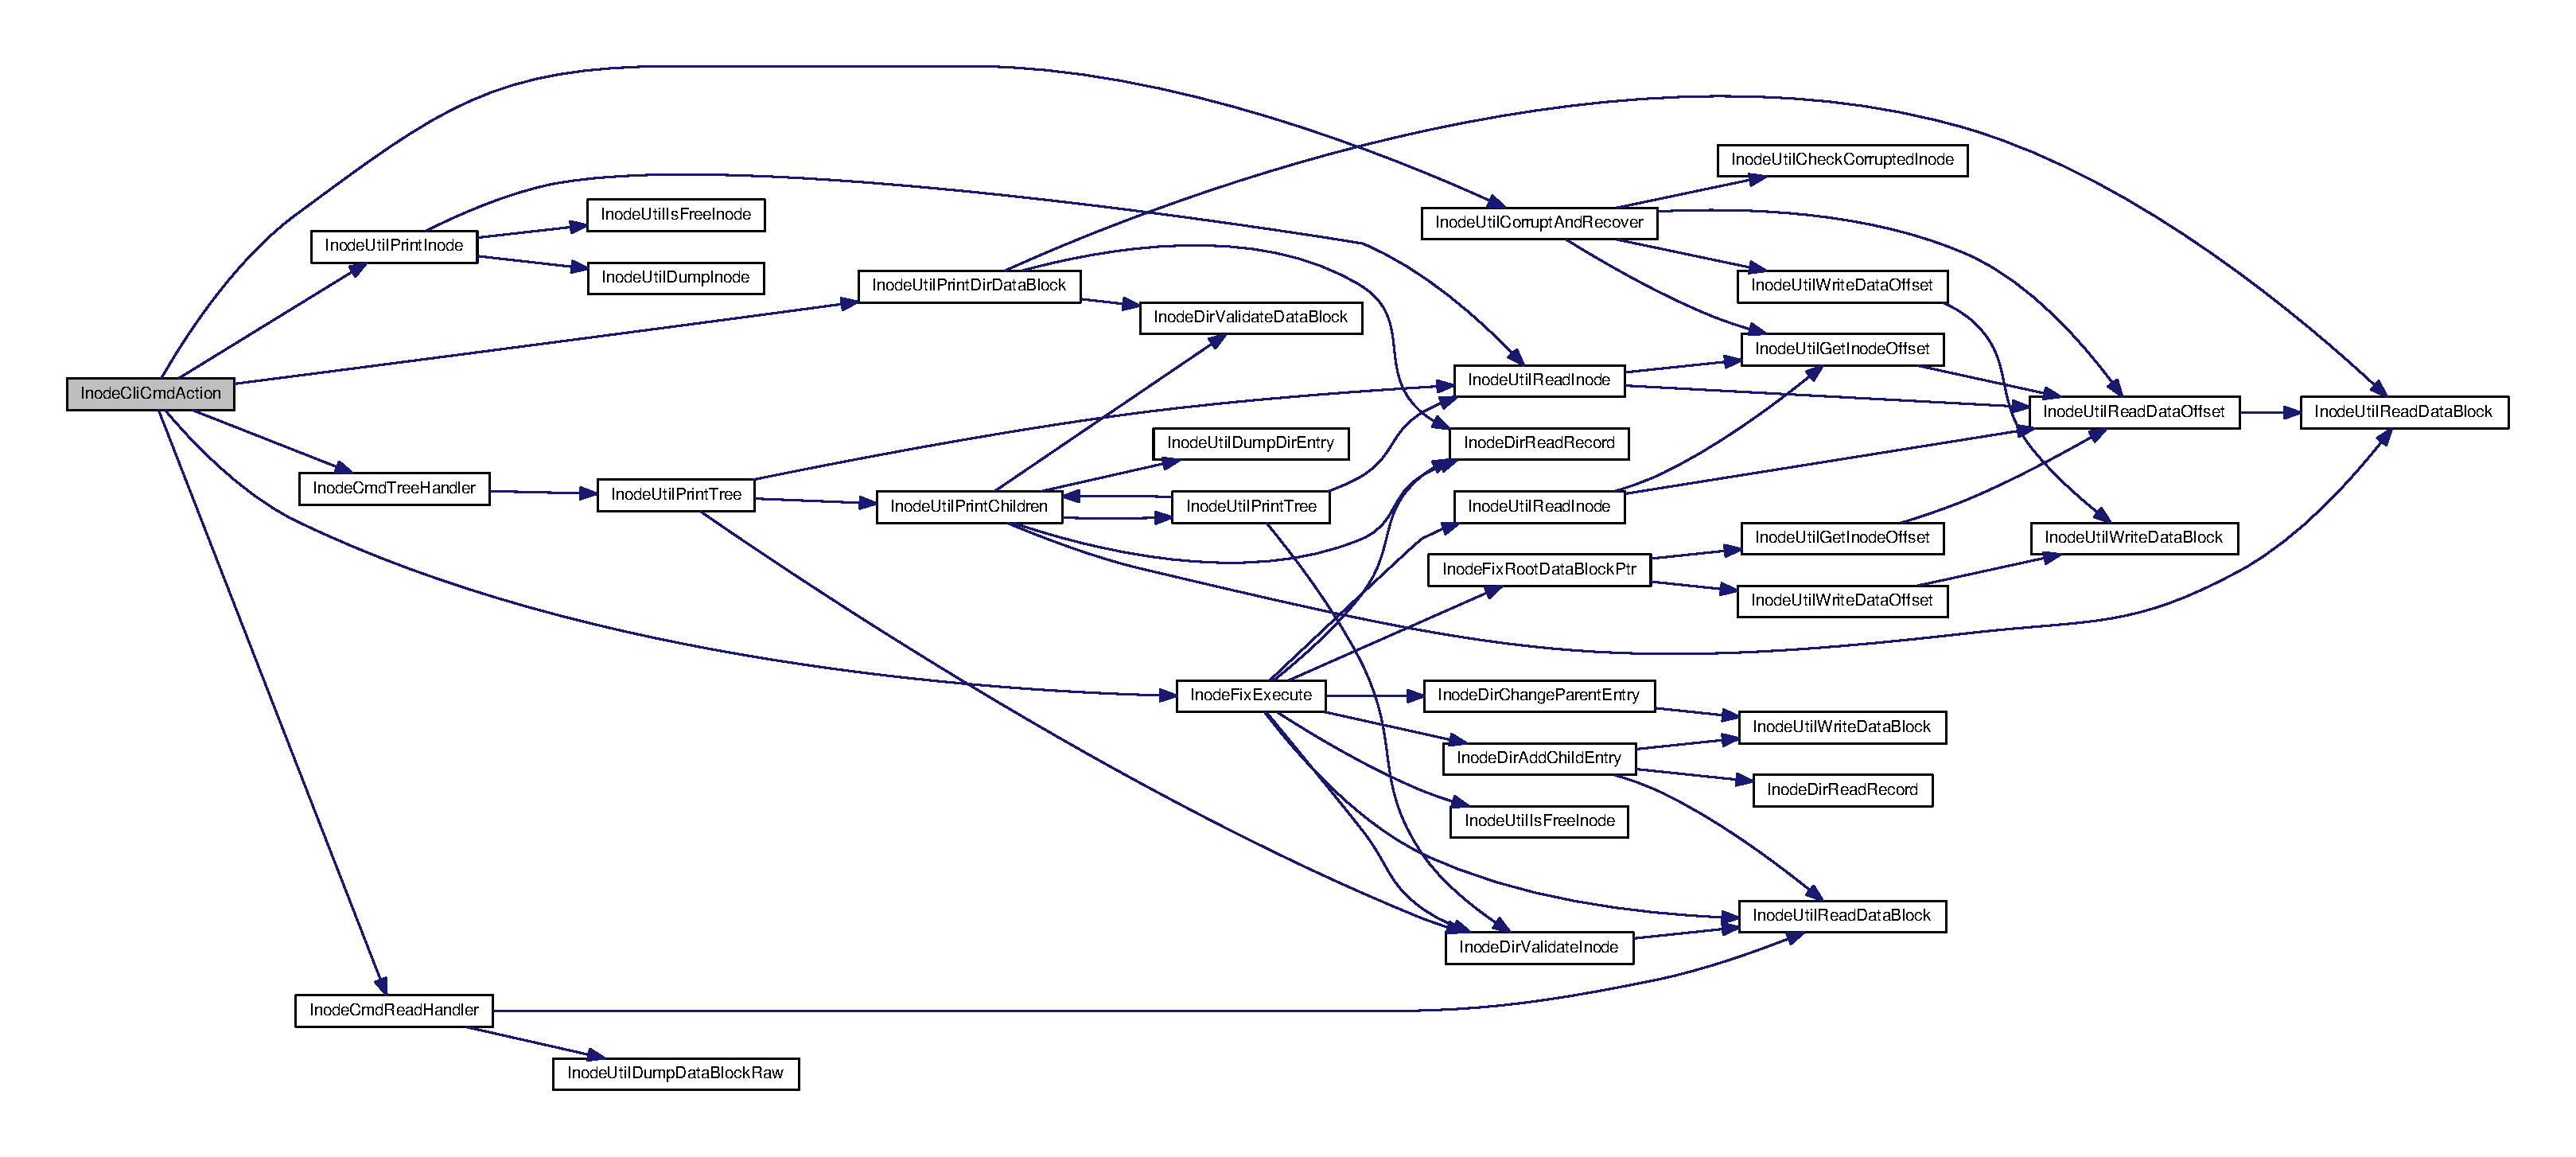
\includegraphics[width=350pt]{inodecli_8h_a3157714cddf8864e002915be47a6cef5_cgraph}
\end{center}
\end{figure}


\hypertarget{inodecli_8h_adde588bd205c9ef530fa02ef8f48cf69}{\index{inodecli.\+h@{inodecli.\+h}!Inode\+Cli\+Handle\+Cmd@{Inode\+Cli\+Handle\+Cmd}}
\index{Inode\+Cli\+Handle\+Cmd@{Inode\+Cli\+Handle\+Cmd}!inodecli.\+h@{inodecli.\+h}}
\subsubsection[{Inode\+Cli\+Handle\+Cmd}]{\setlength{\rightskip}{0pt plus 5cm}V\+O\+I\+D Inode\+Cli\+Handle\+Cmd (
\begin{DoxyParamCaption}
\item[{C\+H\+A\+R $\ast$}]{p\+Cmd}
\end{DoxyParamCaption}
)}}\label{inodecli_8h_adde588bd205c9ef530fa02ef8f48cf69}


 Function Name \+: Inode\+Cli\+Handle

Description \+: This Function tries to parse the command input and if it succeeds then calls the high level action handler function with the parsed command.

Input \+: p\+Cmd -\/ Command string input from the user

Output \+: None

Returns \+: None 

Here is the call graph for this function\+:\nopagebreak
\begin{figure}[H]
\begin{center}
\leavevmode
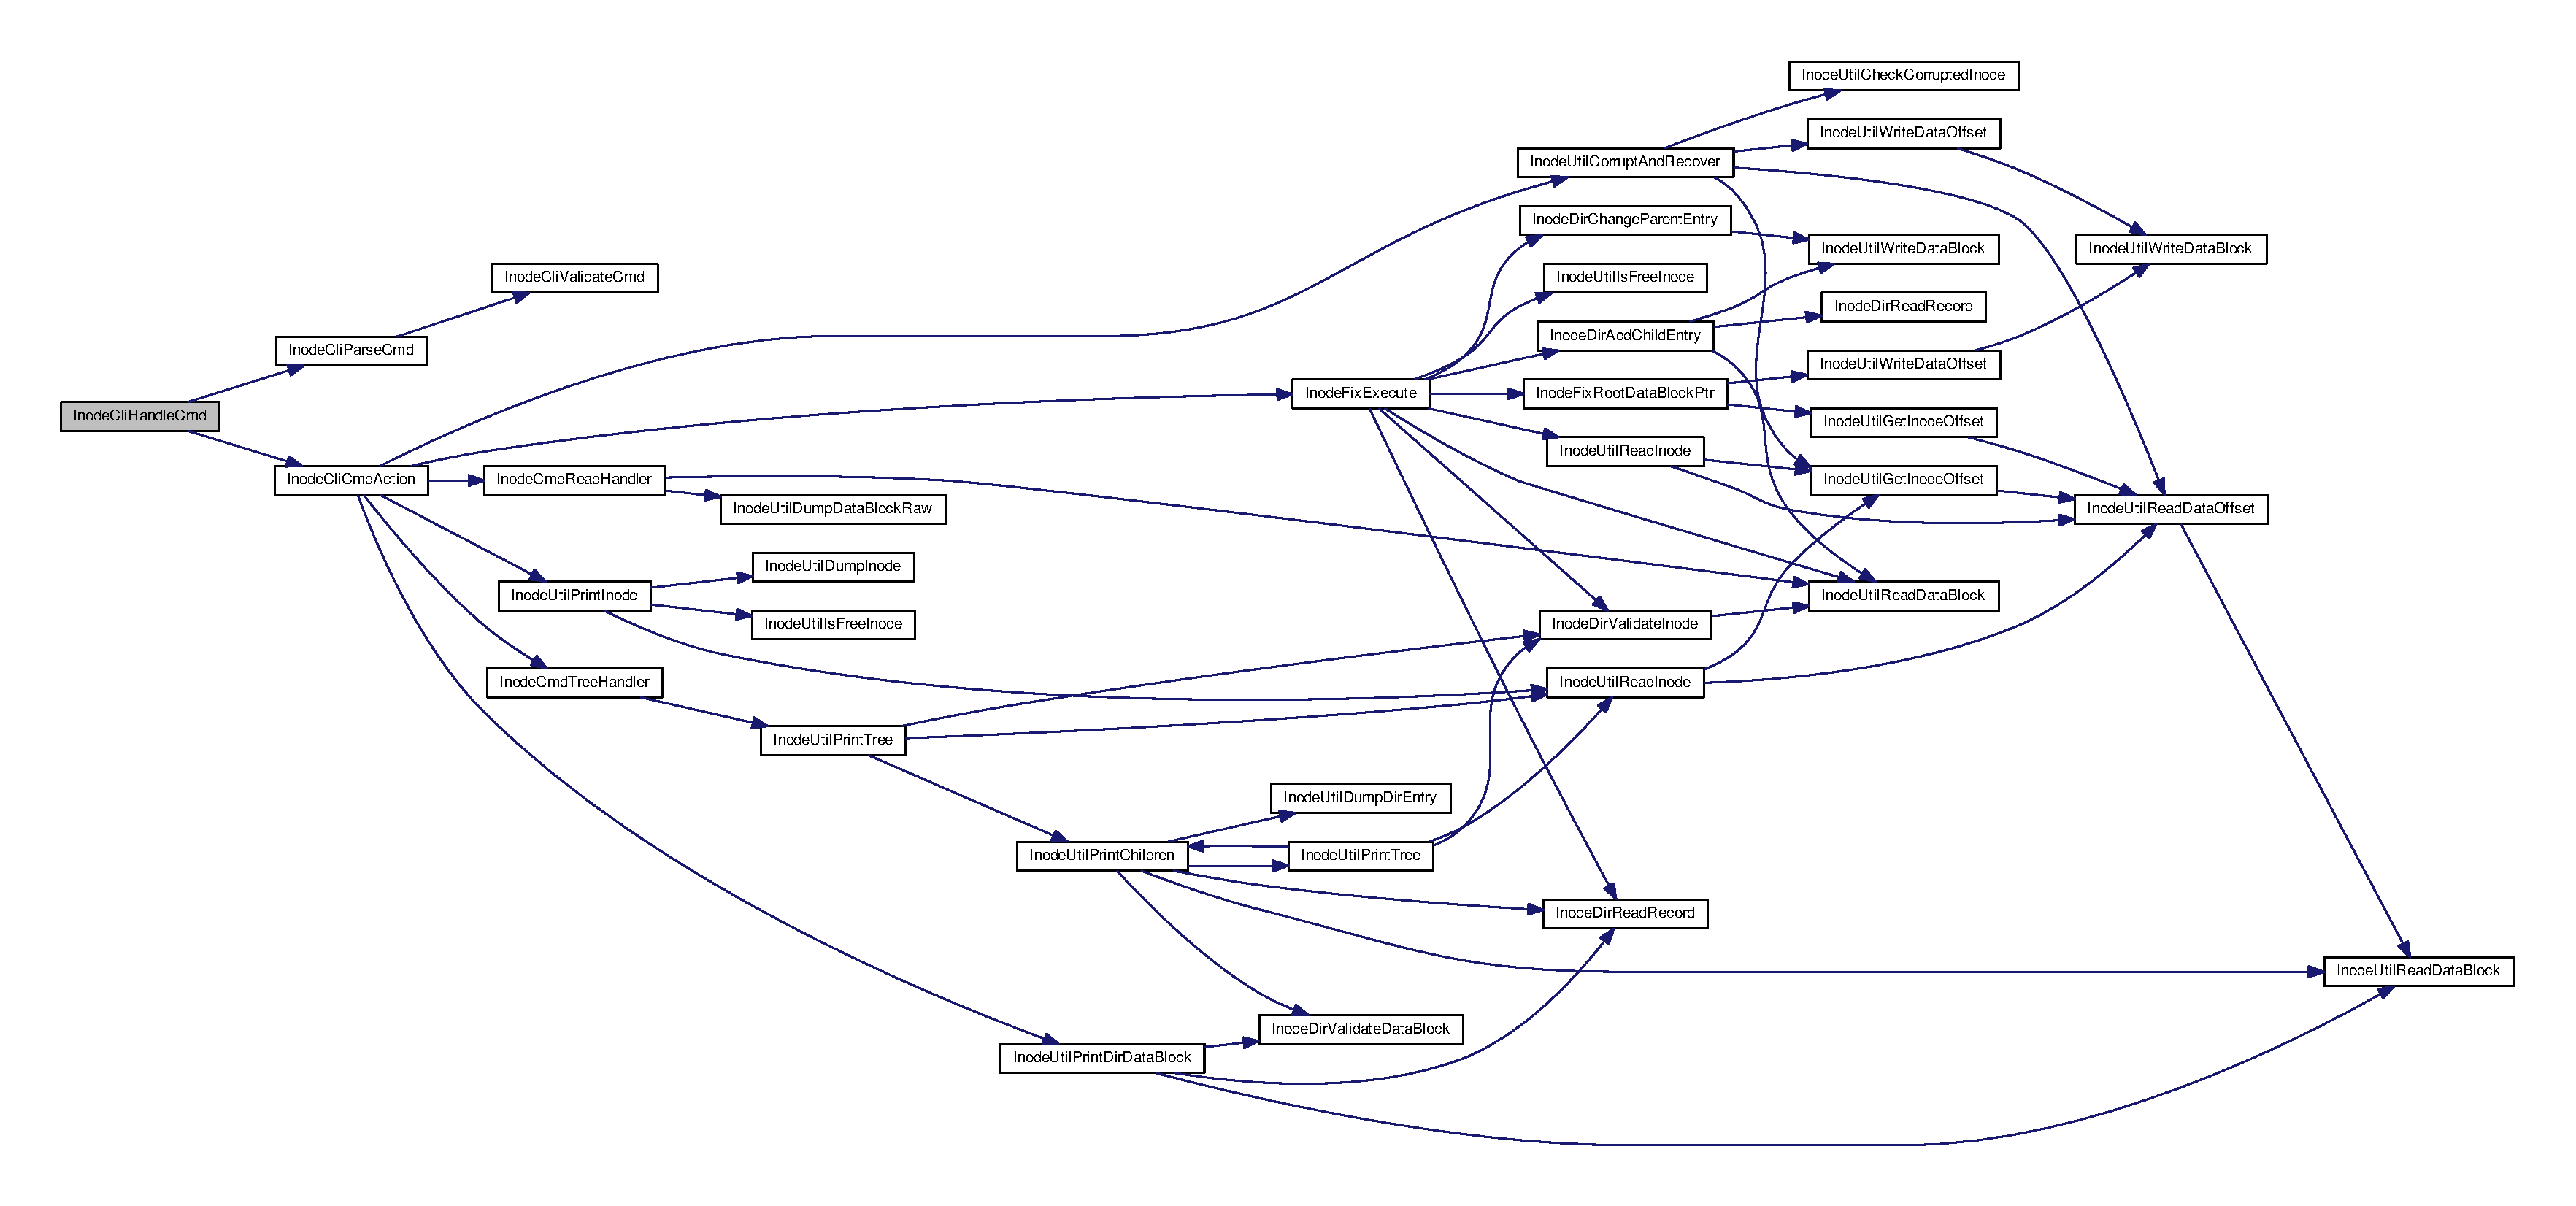
\includegraphics[width=350pt]{inodecli_8h_adde588bd205c9ef530fa02ef8f48cf69_cgraph}
\end{center}
\end{figure}


\hypertarget{inodecli_8h_adaf1a711f6592434c4f1280c0a92fd22}{\index{inodecli.\+h@{inodecli.\+h}!Inode\+Cli\+Parse\+Cmd@{Inode\+Cli\+Parse\+Cmd}}
\index{Inode\+Cli\+Parse\+Cmd@{Inode\+Cli\+Parse\+Cmd}!inodecli.\+h@{inodecli.\+h}}
\subsubsection[{Inode\+Cli\+Parse\+Cmd}]{\setlength{\rightskip}{0pt plus 5cm}I\+N\+T1 Inode\+Cli\+Parse\+Cmd (
\begin{DoxyParamCaption}
\item[{C\+H\+A\+R $\ast$}]{p\+Cmd\+Str, }
\item[{{\bf t\+Command} $\ast$}]{p\+Cmd}
\end{DoxyParamCaption}
)}}\label{inodecli_8h_adaf1a711f6592434c4f1280c0a92fd22}


 Function Name \+: Inode\+Cli\+Parse\+Cmd

Description \+: This Function is used to parse the input command string into the command and arguments.

Input \+: p\+Cmd\+Str -\/ input command string

Output \+: p\+Cmd -\/ structure containing parsed command and arguments

Returns \+: T\+R\+U\+E, if parsing and validation succeeds F\+A\+L\+S\+E otherwise 

Here is the call graph for this function\+:\nopagebreak
\begin{figure}[H]
\begin{center}
\leavevmode
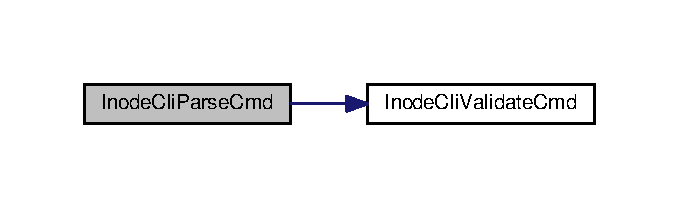
\includegraphics[width=326pt]{inodecli_8h_adaf1a711f6592434c4f1280c0a92fd22_cgraph}
\end{center}
\end{figure}


\hypertarget{inodecli_8h_aa0b53520e1018955fde7aea285159808}{\index{inodecli.\+h@{inodecli.\+h}!Inode\+Cli\+Start@{Inode\+Cli\+Start}}
\index{Inode\+Cli\+Start@{Inode\+Cli\+Start}!inodecli.\+h@{inodecli.\+h}}
\subsubsection[{Inode\+Cli\+Start}]{\setlength{\rightskip}{0pt plus 5cm}V\+O\+I\+D Inode\+Cli\+Start (
\begin{DoxyParamCaption}
{}
\end{DoxyParamCaption}
)}}\label{inodecli_8h_aa0b53520e1018955fde7aea285159808}


 Function Name \+: Inode\+Cli\+Start

Description \+: This Function is used to start the command line interface. This function reads the command input from the user and initiates the action for the command.

Input \+: None

Output \+: None

Returns \+: None 

Here is the call graph for this function\+:\nopagebreak
\begin{figure}[H]
\begin{center}
\leavevmode
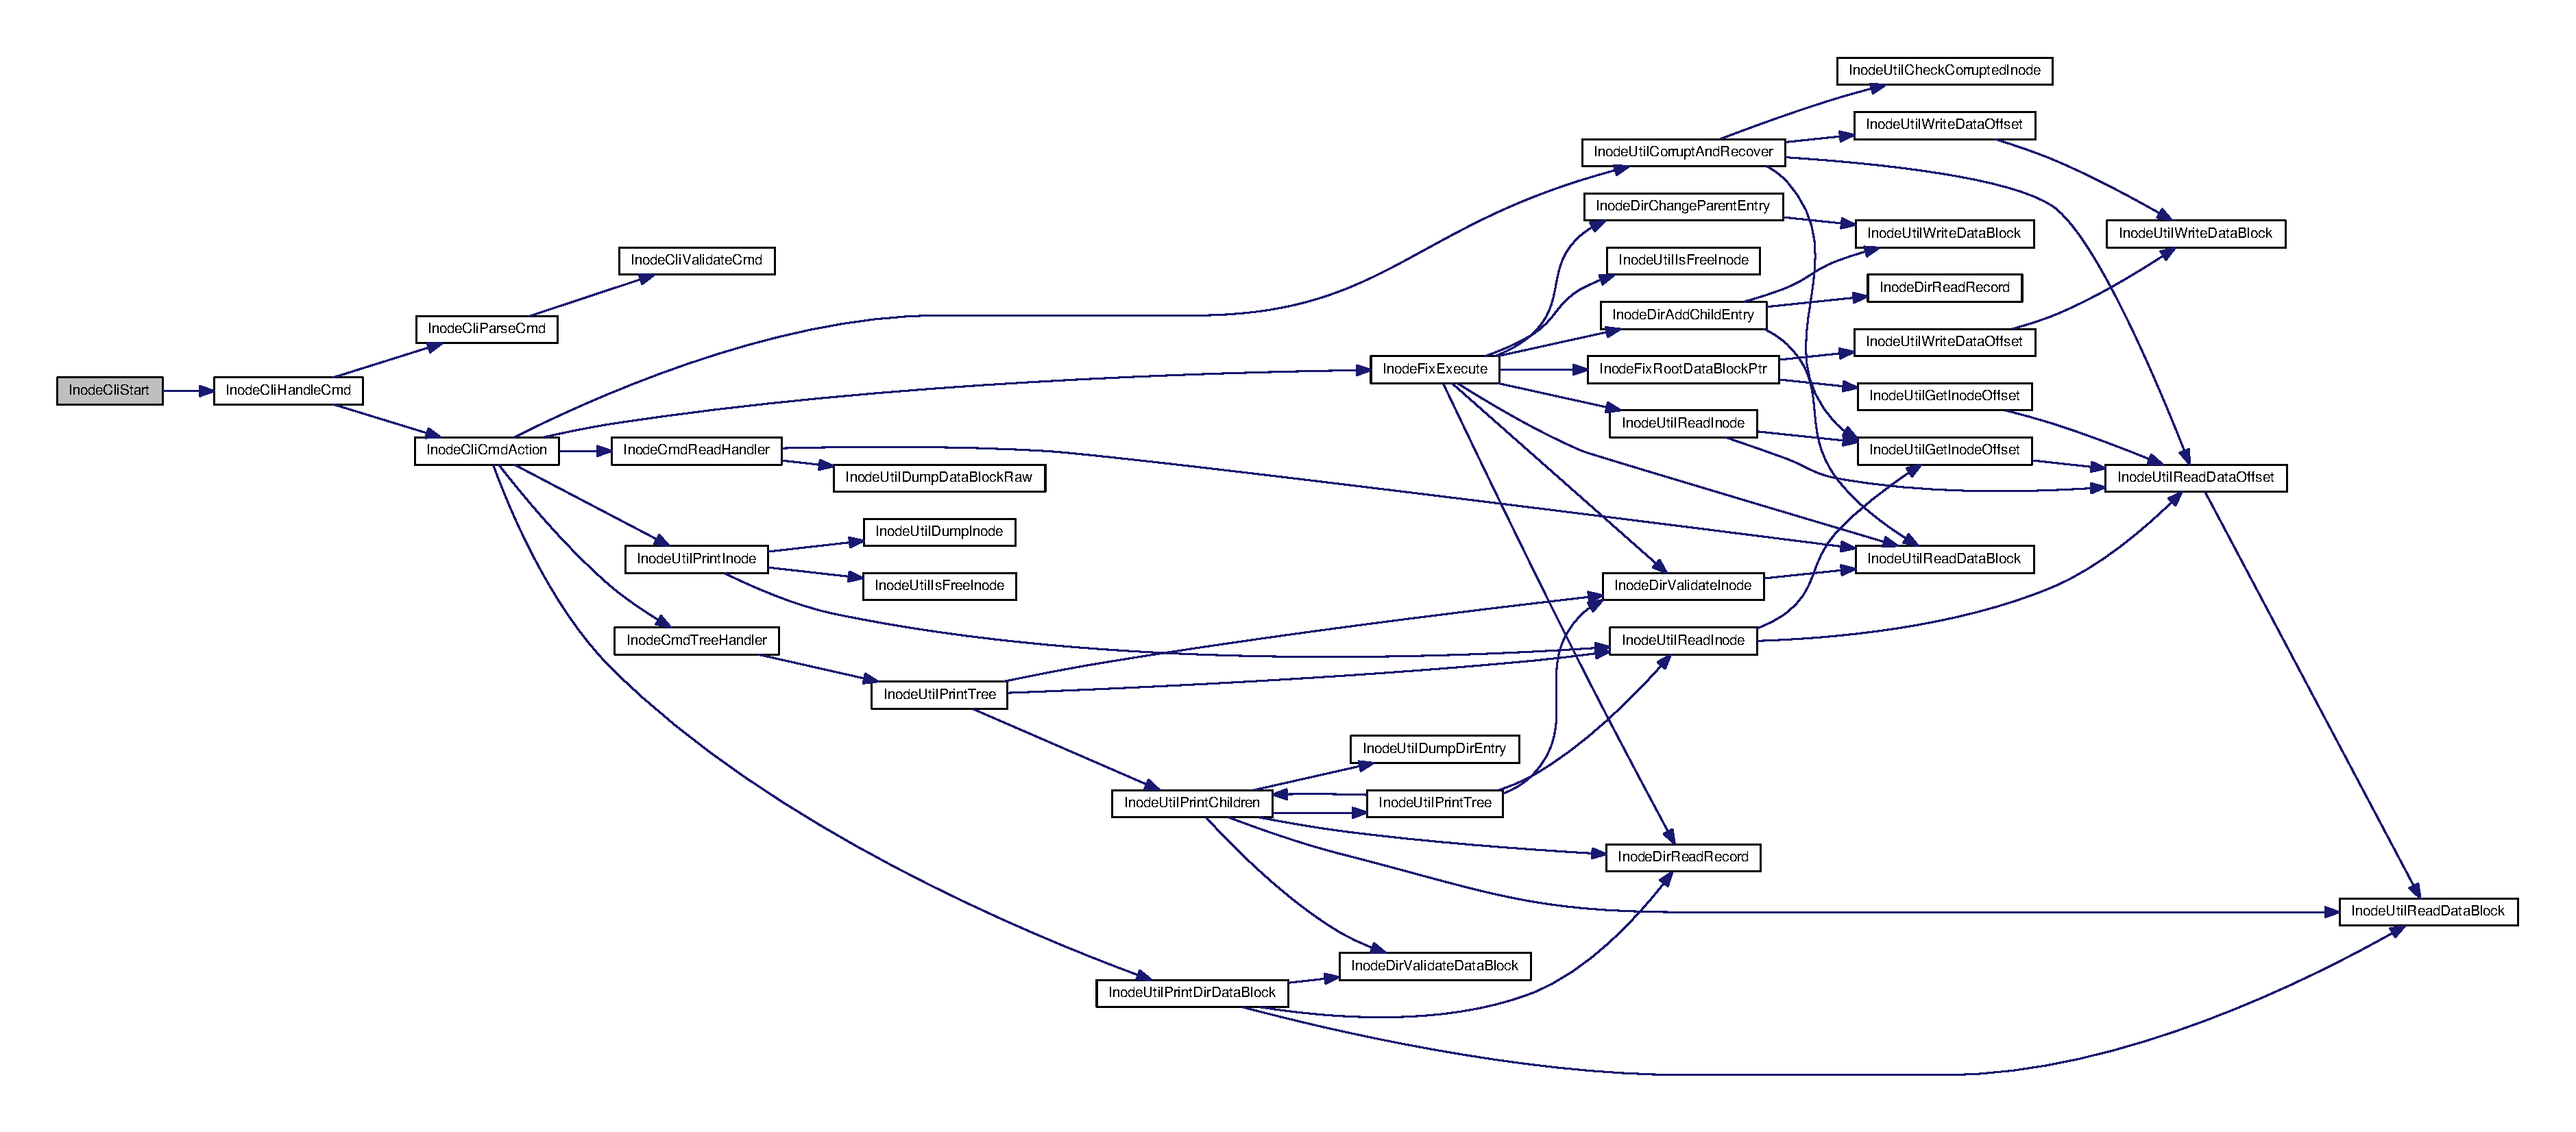
\includegraphics[width=350pt]{inodecli_8h_aa0b53520e1018955fde7aea285159808_cgraph}
\end{center}
\end{figure}


\hypertarget{inodecli_8h_a7d2b674c246cdf3d17a7d091c5f187f8}{\index{inodecli.\+h@{inodecli.\+h}!Inode\+Cli\+Validate\+Cmd@{Inode\+Cli\+Validate\+Cmd}}
\index{Inode\+Cli\+Validate\+Cmd@{Inode\+Cli\+Validate\+Cmd}!inodecli.\+h@{inodecli.\+h}}
\subsubsection[{Inode\+Cli\+Validate\+Cmd}]{\setlength{\rightskip}{0pt plus 5cm}I\+N\+T1 Inode\+Cli\+Validate\+Cmd (
\begin{DoxyParamCaption}
\item[{{\bf t\+Command} $\ast$}]{p\+Cmd, }
\item[{U\+I\+N\+T1}]{u1\+Arg\+C}
\end{DoxyParamCaption}
)}}\label{inodecli_8h_a7d2b674c246cdf3d17a7d091c5f187f8}


 Function Name \+: Inode\+Cli\+Validate\+Cmd

Description \+: This Function is used to validate the parsed command and arguments

Input \+: p\+Cmd -\/ pointer to the parsed command structure u1\+Arg\+C -\/ no. of arguments in the command input

Output \+: None

Returns \+: T\+R\+U\+E, if validation succeeds F\+A\+L\+S\+E otherwise \hypertarget{inodecli_8h_a1635e6bd723f78d1355e30c815348a34}{\index{inodecli.\+h@{inodecli.\+h}!Inode\+Cmd\+Read\+Handler@{Inode\+Cmd\+Read\+Handler}}
\index{Inode\+Cmd\+Read\+Handler@{Inode\+Cmd\+Read\+Handler}!inodecli.\+h@{inodecli.\+h}}
\subsubsection[{Inode\+Cmd\+Read\+Handler}]{\setlength{\rightskip}{0pt plus 5cm}V\+O\+I\+D Inode\+Cmd\+Read\+Handler (
\begin{DoxyParamCaption}
\item[{U\+I\+N\+T4}]{u4\+Block\+No}
\end{DoxyParamCaption}
)}}\label{inodecli_8h_a1635e6bd723f78d1355e30c815348a34}


 Function Name \+: Inode\+Cmd\+Read\+Handler

Description \+: This is the handler function for the command 'read'. This function reads the block specified and prints the contents in H\+E\+X.

Input \+: u4\+Block\+No -\/ Block number to read.

Output \+: None

Returns \+: None 

Here is the call graph for this function\+:\nopagebreak
\begin{figure}[H]
\begin{center}
\leavevmode
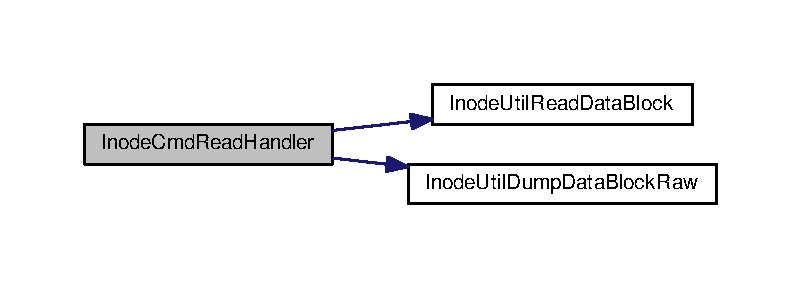
\includegraphics[width=350pt]{inodecli_8h_a1635e6bd723f78d1355e30c815348a34_cgraph}
\end{center}
\end{figure}


\hypertarget{inodecli_8h_a1869e2775252da9a36ecca18ce8198d1}{\index{inodecli.\+h@{inodecli.\+h}!Inode\+Cmd\+Tree\+Handler@{Inode\+Cmd\+Tree\+Handler}}
\index{Inode\+Cmd\+Tree\+Handler@{Inode\+Cmd\+Tree\+Handler}!inodecli.\+h@{inodecli.\+h}}
\subsubsection[{Inode\+Cmd\+Tree\+Handler}]{\setlength{\rightskip}{0pt plus 5cm}V\+O\+I\+D Inode\+Cmd\+Tree\+Handler (
\begin{DoxyParamCaption}
\item[{U\+I\+N\+T4}]{u4\+Inode\+No}
\end{DoxyParamCaption}
)}}\label{inodecli_8h_a1869e2775252da9a36ecca18ce8198d1}


 Function Name \+: Inode\+Cmd\+Tree\+Handler

Description \+: This is the handler function for the command 'tree'. This function prints the directory/files tree starting at the given inode.

Input \+: u4\+Inode\+No -\/ Root inode to start.

Output \+: None

Returns \+: None 

Here is the call graph for this function\+:\nopagebreak
\begin{figure}[H]
\begin{center}
\leavevmode
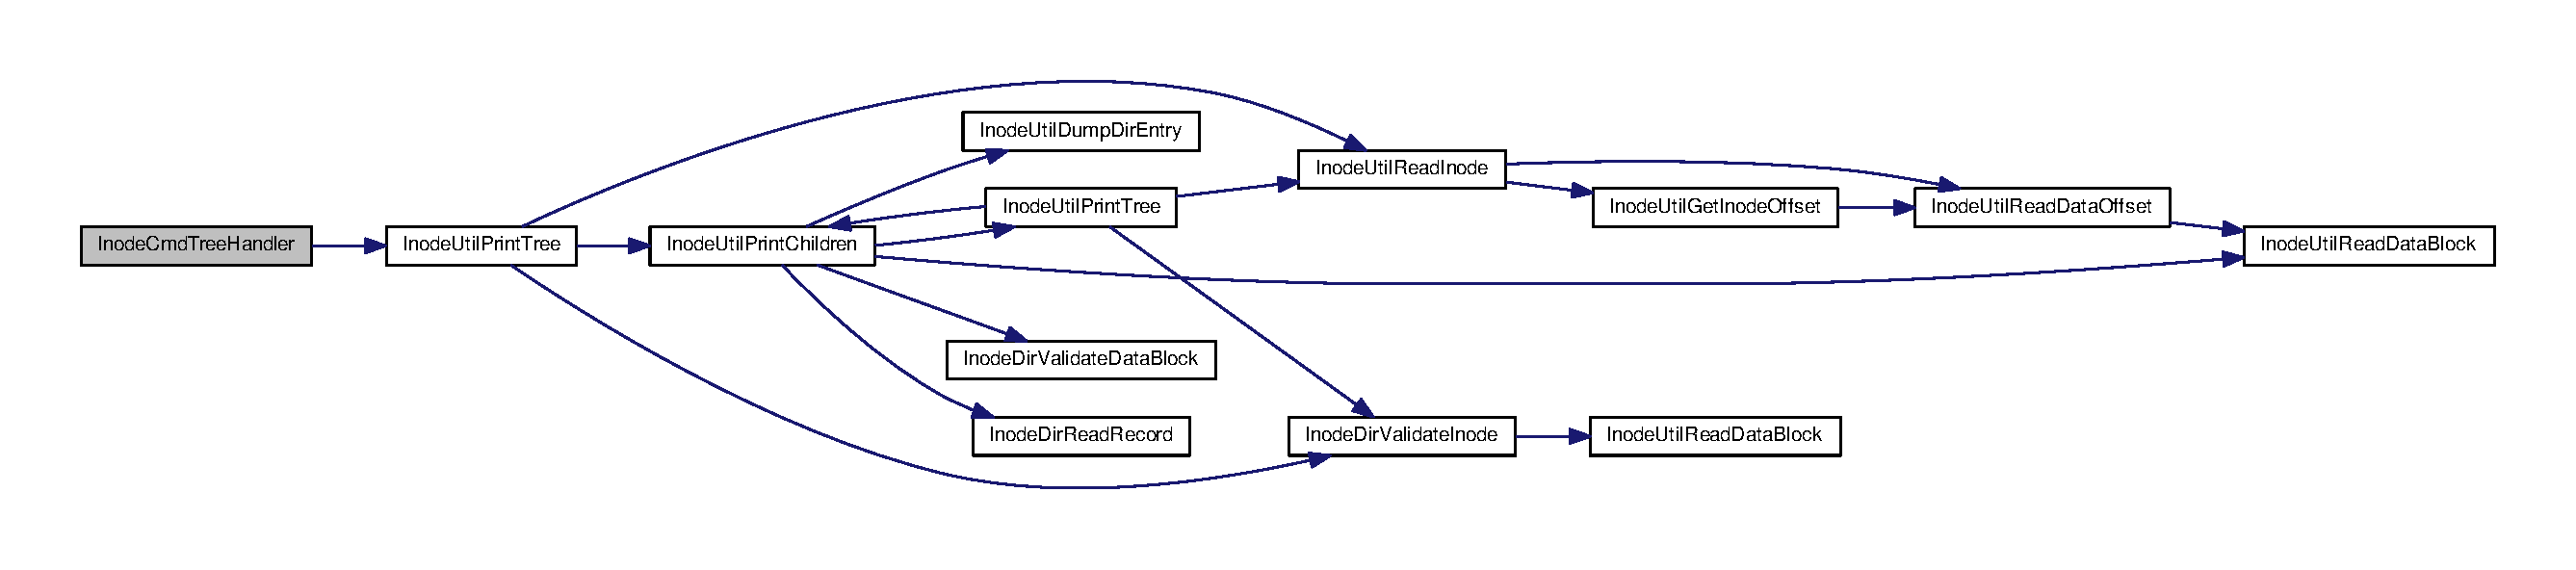
\includegraphics[width=350pt]{inodecli_8h_a1869e2775252da9a36ecca18ce8198d1_cgraph}
\end{center}
\end{figure}



\hypertarget{inodedef_8h}{\section{inc/inodedef.h File Reference}
\label{inodedef_8h}\index{inc/inodedef.\+h@{inc/inodedef.\+h}}
}
This graph shows which files directly or indirectly include this file\+:\nopagebreak
\begin{figure}[H]
\begin{center}
\leavevmode
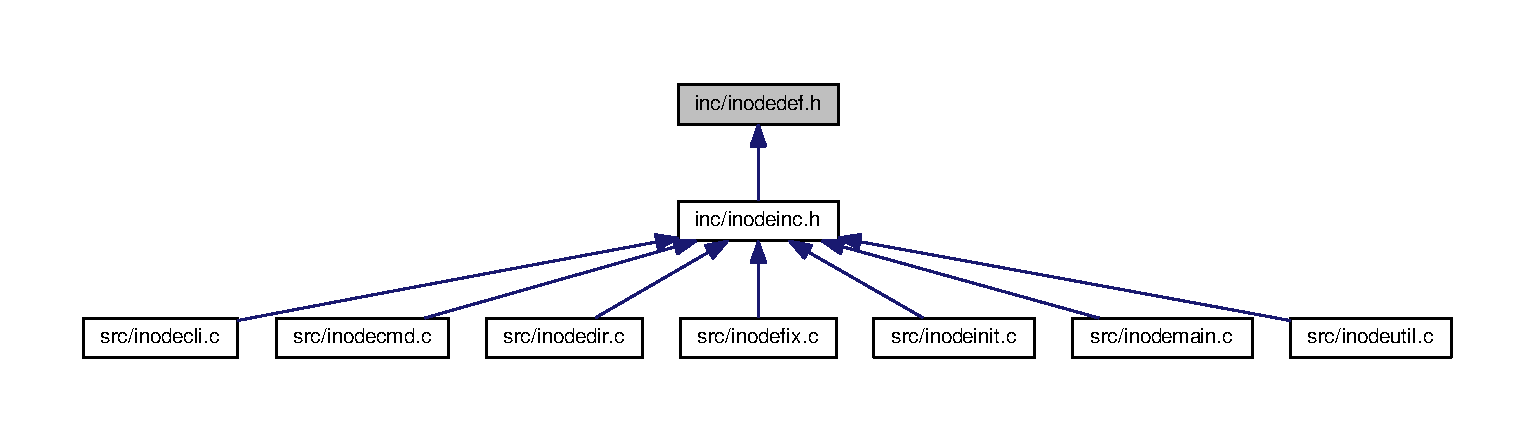
\includegraphics[width=350pt]{inodedef_8h__dep__incl}
\end{center}
\end{figure}
\subsection*{Macros}
\begin{DoxyCompactItemize}
\item 
\#define \hyperlink{inodedef_8h_ae3d6ffb7ce73b92de2e4c01ae5226958}{B\+O\+O\+T\+\_\+\+S\+E\+C\+T\+O\+R\+\_\+\+O\+F\+F\+S\+E\+T}~1024
\item 
\#define \hyperlink{inodedef_8h_aeb3268af9dfb0cdb034dae837237fa3b}{D\+I\+R\+\_\+\+N\+A\+M\+E\+\_\+\+P\+A\+R\+E\+N\+T}~\char`\"{}..\char`\"{}
\item 
\#define \hyperlink{inodedef_8h_a8dd3432df729722cd2ac4ae94ef732ec}{D\+I\+R\+\_\+\+N\+A\+M\+E\+\_\+\+C\+U\+R\+R\+E\+N\+T}~\char`\"{}.\char`\"{}
\item 
\#define \hyperlink{inodedef_8h_a7093e5962ec18fdb76d7ce02668f35bc}{D\+I\+R\+\_\+\+C\+U\+R\+R\+\_\+\+E\+N\+T\+R\+Y\+\_\+\+O\+F\+F\+S\+E\+T}~0
\item 
\#define \hyperlink{inodedef_8h_a0af6d872db5b784e4d9c349e44f65c77}{D\+I\+R\+\_\+\+P\+A\+R\+E\+N\+T\+\_\+\+E\+N\+T\+R\+Y\+\_\+\+O\+F\+F\+S\+E\+T}~12
\item 
\#define \hyperlink{inodedef_8h_a55b46cda1b6f1dd22012409cf25a3eb1}{D\+I\+R\+\_\+\+C\+U\+R\+R\+\_\+\+E\+N\+T\+R\+Y\+\_\+\+S\+I\+Z\+E}~12
\item 
\#define \hyperlink{inodedef_8h_ae56994282466f8af08da5f62b052230f}{D\+I\+R\+\_\+\+P\+A\+R\+E\+N\+T\+\_\+\+E\+N\+T\+R\+Y\+\_\+\+S\+I\+Z\+E}~12
\item 
\#define \hyperlink{inodedef_8h_a3818ff77519fd704ec32036a20f504de}{D\+I\+R\+\_\+\+E\+N\+T\+R\+Y\+\_\+\+N\+A\+M\+E\+\_\+\+O\+F\+F\+S\+E\+T}~sizeof(U\+I\+N\+T8)
\item 
\#define \hyperlink{inodedef_8h_a6ab4716428c2bdc69702df81852e055b}{I\+N\+O\+D\+E\+\_\+\+S\+U\+C\+C\+E\+S\+S}~1
\item 
\#define \hyperlink{inodedef_8h_a01d6160e32baf34fc2183aff35c917b6}{I\+N\+O\+D\+E\+\_\+\+F\+A\+I\+L\+U\+R\+E}~-\/1
\item 
\#define \hyperlink{inodedef_8h_a6fefb99a279054362ece826744775d7d}{R\+O\+O\+T\+\_\+\+I\+N\+O\+D\+E}~2
\item 
\#define \hyperlink{inodedef_8h_a22f091dfb43508b0274af4c84e658b7c}{R\+E\+C\+\_\+\+N\+A\+M\+E\+\_\+\+P\+R\+E\+F\+I\+X}~\char`\"{}Recovery\+\_\+\char`\"{}
\item 
\#define \hyperlink{inodedef_8h_aa8bad2cd89820cdaf2a7f26392774014}{M\+A\+X\+\_\+\+B\+L\+O\+C\+K\+\_\+\+S\+I\+Z\+E}
\item 
\#define \hyperlink{inodedef_8h_ae3b0854a3c149a5350a54c1ec475475a}{D\+I\+R\+\_\+\+C\+R\+E\+A\+T\+E}(New\+Dir\+Entry, Inode, Name, File\+Type)
\item 
\#define \hyperlink{inodedef_8h_adfd22f3c30f58a0a8f0ff6a2d1077b34}{D\+I\+R\+\_\+\+R\+E\+C\+\_\+\+L\+E\+N}(Dir\+Entry)
\item 
\#define \hyperlink{inodedef_8h_aa42e059eb1c65a67ae0a223128299a77}{M\+A\+X\+\_\+\+C\+O\+R\+R\+\_\+\+I\+N\+O\+D\+E\+S}~100
\item 
\#define \hyperlink{inodedef_8h_ad43f7aff7a46e3d39ea16d4571ebd5fa}{D\+I\+R\+E\+C\+T\+\_\+\+B\+L\+O\+C\+K\+\_\+\+O\+F\+F\+S\+E\+T}~0x28  /$\ast$ offset for i\+\_\+block\mbox{[}0\mbox{]} from inode offset $\ast$/
\item 
\#define \hyperlink{inodedef_8h_af2583944dd05446b72bd4e897f4c8496}{C\+O\+R\+R\+\_\+\+F\+I\+X\+\_\+\+M\+A\+S\+K}~0x15  /$\ast$ mask to corrupt and recover data \+: corrupting 1,3,5 of L\+S\+B $\ast$/
\item 
\#define \hyperlink{inodedef_8h_aec93e83855ac17c3c25c55c37ca186dd}{B\+Y\+T\+E}~8
\item 
\#define \hyperlink{inodedef_8h_aff8bcf60af0cce430f7c7c7883d25e9a}{M\+A\+X\+\_\+\+I\+N\+O\+D\+E\+\_\+\+A\+R\+R\+A\+Y\+\_\+\+S\+I\+Z\+E}~(ceil((float)\hyperlink{inodeglob_8h_a901acbb8d2da8400086899838bba175d}{gu4\+Total\+Inodes} / \hyperlink{inodedef_8h_aec93e83855ac17c3c25c55c37ca186dd}{B\+Y\+T\+E}))
\item 
\#define \hyperlink{inodedef_8h_a4a7a48f7c935365862c629f61afead35}{M\+A\+S\+K\+\_\+\+B\+I\+T\+\_\+0}~0x80 /$\ast$ M\+S\+B $\ast$/
\item 
\#define \hyperlink{inodedef_8h_af9804ff1f7b256607a55792739574405}{M\+A\+S\+K\+\_\+\+B\+I\+T\+\_\+1}~0x40
\item 
\#define \hyperlink{inodedef_8h_a022d71fcd989b20f6bdde3db45a7d303}{M\+A\+S\+K\+\_\+\+B\+I\+T\+\_\+2}~0x20
\item 
\#define \hyperlink{inodedef_8h_a79677d336ccddc25443bf56448283f00}{M\+A\+S\+K\+\_\+\+B\+I\+T\+\_\+3}~0x10
\item 
\#define \hyperlink{inodedef_8h_aa2322a25c802891d09d699d0f645ae96}{M\+A\+S\+K\+\_\+\+B\+I\+T\+\_\+4}~0x08
\item 
\#define \hyperlink{inodedef_8h_a50e5e36f14609e9f4c4c21e23fbfeac0}{M\+A\+S\+K\+\_\+\+B\+I\+T\+\_\+5}~0x04
\item 
\#define \hyperlink{inodedef_8h_ab2d473aba70919c2c88422e3ea816816}{M\+A\+S\+K\+\_\+\+B\+I\+T\+\_\+6}~0x02
\item 
\#define \hyperlink{inodedef_8h_a6901ab2495ba75259a83782ed2f4b5a8}{M\+A\+S\+K\+\_\+\+B\+I\+T\+\_\+7}~0x01 /$\ast$ L\+S\+B $\ast$/
\item 
\#define \hyperlink{inodedef_8h_af1b4af3d72bf7a539e20e4b3ce13b6d8}{G\+E\+T\+\_\+\+B\+L\+O\+C\+K\+\_\+\+O\+F\+F\+S\+E\+T\+\_\+\+F\+R\+O\+M\+\_\+\+B\+Y\+T\+E\+\_\+\+O\+F\+F\+S\+E\+T}(Block, Position, Byte\+Offset)
\end{DoxyCompactItemize}


\subsection{Macro Definition Documentation}
\hypertarget{inodedef_8h_ae3d6ffb7ce73b92de2e4c01ae5226958}{\index{inodedef.\+h@{inodedef.\+h}!B\+O\+O\+T\+\_\+\+S\+E\+C\+T\+O\+R\+\_\+\+O\+F\+F\+S\+E\+T@{B\+O\+O\+T\+\_\+\+S\+E\+C\+T\+O\+R\+\_\+\+O\+F\+F\+S\+E\+T}}
\index{B\+O\+O\+T\+\_\+\+S\+E\+C\+T\+O\+R\+\_\+\+O\+F\+F\+S\+E\+T@{B\+O\+O\+T\+\_\+\+S\+E\+C\+T\+O\+R\+\_\+\+O\+F\+F\+S\+E\+T}!inodedef.\+h@{inodedef.\+h}}
\subsubsection[{B\+O\+O\+T\+\_\+\+S\+E\+C\+T\+O\+R\+\_\+\+O\+F\+F\+S\+E\+T}]{\setlength{\rightskip}{0pt plus 5cm}\#define B\+O\+O\+T\+\_\+\+S\+E\+C\+T\+O\+R\+\_\+\+O\+F\+F\+S\+E\+T~1024}}\label{inodedef_8h_ae3d6ffb7ce73b92de2e4c01ae5226958}
\hypertarget{inodedef_8h_aec93e83855ac17c3c25c55c37ca186dd}{\index{inodedef.\+h@{inodedef.\+h}!B\+Y\+T\+E@{B\+Y\+T\+E}}
\index{B\+Y\+T\+E@{B\+Y\+T\+E}!inodedef.\+h@{inodedef.\+h}}
\subsubsection[{B\+Y\+T\+E}]{\setlength{\rightskip}{0pt plus 5cm}\#define B\+Y\+T\+E~8}}\label{inodedef_8h_aec93e83855ac17c3c25c55c37ca186dd}
\hypertarget{inodedef_8h_af2583944dd05446b72bd4e897f4c8496}{\index{inodedef.\+h@{inodedef.\+h}!C\+O\+R\+R\+\_\+\+F\+I\+X\+\_\+\+M\+A\+S\+K@{C\+O\+R\+R\+\_\+\+F\+I\+X\+\_\+\+M\+A\+S\+K}}
\index{C\+O\+R\+R\+\_\+\+F\+I\+X\+\_\+\+M\+A\+S\+K@{C\+O\+R\+R\+\_\+\+F\+I\+X\+\_\+\+M\+A\+S\+K}!inodedef.\+h@{inodedef.\+h}}
\subsubsection[{C\+O\+R\+R\+\_\+\+F\+I\+X\+\_\+\+M\+A\+S\+K}]{\setlength{\rightskip}{0pt plus 5cm}\#define C\+O\+R\+R\+\_\+\+F\+I\+X\+\_\+\+M\+A\+S\+K~0x15  /$\ast$ mask to corrupt and recover data \+: corrupting 1,3,5 of L\+S\+B $\ast$/}}\label{inodedef_8h_af2583944dd05446b72bd4e897f4c8496}
\hypertarget{inodedef_8h_ae3b0854a3c149a5350a54c1ec475475a}{\index{inodedef.\+h@{inodedef.\+h}!D\+I\+R\+\_\+\+C\+R\+E\+A\+T\+E@{D\+I\+R\+\_\+\+C\+R\+E\+A\+T\+E}}
\index{D\+I\+R\+\_\+\+C\+R\+E\+A\+T\+E@{D\+I\+R\+\_\+\+C\+R\+E\+A\+T\+E}!inodedef.\+h@{inodedef.\+h}}
\subsubsection[{D\+I\+R\+\_\+\+C\+R\+E\+A\+T\+E}]{\setlength{\rightskip}{0pt plus 5cm}\#define D\+I\+R\+\_\+\+C\+R\+E\+A\+T\+E(
\begin{DoxyParamCaption}
\item[{}]{New\+Dir\+Entry, }
\item[{}]{Inode, }
\item[{}]{Name, }
\item[{}]{File\+Type}
\end{DoxyParamCaption}
)}}\label{inodedef_8h_ae3b0854a3c149a5350a54c1ec475475a}
{\bfseries Value\+:}
\begin{DoxyCode}
NewDirEntry.inode = Inode; \(\backslash\)
                                NewDirEntry.file\_type = FileType; \(\backslash\)
                strncpy(NewDirEntry.name, Name, strlen(Name)); \(\backslash\)
                NewDirEntry.name\_len = strlen(NewDirEntry.name); \(\backslash\)
                NewDirEntry.rec\_len = ceil((\textcolor{keywordtype}{float})(DirEntry.name\_len + 
      \hyperlink{inodedef_8h_a3818ff77519fd704ec32036a20f504de}{DIR\_ENTRY\_NAME\_OFFSET}) / 4) * 4;
\end{DoxyCode}
\hypertarget{inodedef_8h_a7093e5962ec18fdb76d7ce02668f35bc}{\index{inodedef.\+h@{inodedef.\+h}!D\+I\+R\+\_\+\+C\+U\+R\+R\+\_\+\+E\+N\+T\+R\+Y\+\_\+\+O\+F\+F\+S\+E\+T@{D\+I\+R\+\_\+\+C\+U\+R\+R\+\_\+\+E\+N\+T\+R\+Y\+\_\+\+O\+F\+F\+S\+E\+T}}
\index{D\+I\+R\+\_\+\+C\+U\+R\+R\+\_\+\+E\+N\+T\+R\+Y\+\_\+\+O\+F\+F\+S\+E\+T@{D\+I\+R\+\_\+\+C\+U\+R\+R\+\_\+\+E\+N\+T\+R\+Y\+\_\+\+O\+F\+F\+S\+E\+T}!inodedef.\+h@{inodedef.\+h}}
\subsubsection[{D\+I\+R\+\_\+\+C\+U\+R\+R\+\_\+\+E\+N\+T\+R\+Y\+\_\+\+O\+F\+F\+S\+E\+T}]{\setlength{\rightskip}{0pt plus 5cm}\#define D\+I\+R\+\_\+\+C\+U\+R\+R\+\_\+\+E\+N\+T\+R\+Y\+\_\+\+O\+F\+F\+S\+E\+T~0}}\label{inodedef_8h_a7093e5962ec18fdb76d7ce02668f35bc}
\hypertarget{inodedef_8h_a55b46cda1b6f1dd22012409cf25a3eb1}{\index{inodedef.\+h@{inodedef.\+h}!D\+I\+R\+\_\+\+C\+U\+R\+R\+\_\+\+E\+N\+T\+R\+Y\+\_\+\+S\+I\+Z\+E@{D\+I\+R\+\_\+\+C\+U\+R\+R\+\_\+\+E\+N\+T\+R\+Y\+\_\+\+S\+I\+Z\+E}}
\index{D\+I\+R\+\_\+\+C\+U\+R\+R\+\_\+\+E\+N\+T\+R\+Y\+\_\+\+S\+I\+Z\+E@{D\+I\+R\+\_\+\+C\+U\+R\+R\+\_\+\+E\+N\+T\+R\+Y\+\_\+\+S\+I\+Z\+E}!inodedef.\+h@{inodedef.\+h}}
\subsubsection[{D\+I\+R\+\_\+\+C\+U\+R\+R\+\_\+\+E\+N\+T\+R\+Y\+\_\+\+S\+I\+Z\+E}]{\setlength{\rightskip}{0pt plus 5cm}\#define D\+I\+R\+\_\+\+C\+U\+R\+R\+\_\+\+E\+N\+T\+R\+Y\+\_\+\+S\+I\+Z\+E~12}}\label{inodedef_8h_a55b46cda1b6f1dd22012409cf25a3eb1}
\hypertarget{inodedef_8h_a3818ff77519fd704ec32036a20f504de}{\index{inodedef.\+h@{inodedef.\+h}!D\+I\+R\+\_\+\+E\+N\+T\+R\+Y\+\_\+\+N\+A\+M\+E\+\_\+\+O\+F\+F\+S\+E\+T@{D\+I\+R\+\_\+\+E\+N\+T\+R\+Y\+\_\+\+N\+A\+M\+E\+\_\+\+O\+F\+F\+S\+E\+T}}
\index{D\+I\+R\+\_\+\+E\+N\+T\+R\+Y\+\_\+\+N\+A\+M\+E\+\_\+\+O\+F\+F\+S\+E\+T@{D\+I\+R\+\_\+\+E\+N\+T\+R\+Y\+\_\+\+N\+A\+M\+E\+\_\+\+O\+F\+F\+S\+E\+T}!inodedef.\+h@{inodedef.\+h}}
\subsubsection[{D\+I\+R\+\_\+\+E\+N\+T\+R\+Y\+\_\+\+N\+A\+M\+E\+\_\+\+O\+F\+F\+S\+E\+T}]{\setlength{\rightskip}{0pt plus 5cm}\#define D\+I\+R\+\_\+\+E\+N\+T\+R\+Y\+\_\+\+N\+A\+M\+E\+\_\+\+O\+F\+F\+S\+E\+T~sizeof(U\+I\+N\+T8)}}\label{inodedef_8h_a3818ff77519fd704ec32036a20f504de}
\hypertarget{inodedef_8h_a8dd3432df729722cd2ac4ae94ef732ec}{\index{inodedef.\+h@{inodedef.\+h}!D\+I\+R\+\_\+\+N\+A\+M\+E\+\_\+\+C\+U\+R\+R\+E\+N\+T@{D\+I\+R\+\_\+\+N\+A\+M\+E\+\_\+\+C\+U\+R\+R\+E\+N\+T}}
\index{D\+I\+R\+\_\+\+N\+A\+M\+E\+\_\+\+C\+U\+R\+R\+E\+N\+T@{D\+I\+R\+\_\+\+N\+A\+M\+E\+\_\+\+C\+U\+R\+R\+E\+N\+T}!inodedef.\+h@{inodedef.\+h}}
\subsubsection[{D\+I\+R\+\_\+\+N\+A\+M\+E\+\_\+\+C\+U\+R\+R\+E\+N\+T}]{\setlength{\rightskip}{0pt plus 5cm}\#define D\+I\+R\+\_\+\+N\+A\+M\+E\+\_\+\+C\+U\+R\+R\+E\+N\+T~\char`\"{}.\char`\"{}}}\label{inodedef_8h_a8dd3432df729722cd2ac4ae94ef732ec}
\hypertarget{inodedef_8h_aeb3268af9dfb0cdb034dae837237fa3b}{\index{inodedef.\+h@{inodedef.\+h}!D\+I\+R\+\_\+\+N\+A\+M\+E\+\_\+\+P\+A\+R\+E\+N\+T@{D\+I\+R\+\_\+\+N\+A\+M\+E\+\_\+\+P\+A\+R\+E\+N\+T}}
\index{D\+I\+R\+\_\+\+N\+A\+M\+E\+\_\+\+P\+A\+R\+E\+N\+T@{D\+I\+R\+\_\+\+N\+A\+M\+E\+\_\+\+P\+A\+R\+E\+N\+T}!inodedef.\+h@{inodedef.\+h}}
\subsubsection[{D\+I\+R\+\_\+\+N\+A\+M\+E\+\_\+\+P\+A\+R\+E\+N\+T}]{\setlength{\rightskip}{0pt plus 5cm}\#define D\+I\+R\+\_\+\+N\+A\+M\+E\+\_\+\+P\+A\+R\+E\+N\+T~\char`\"{}..\char`\"{}}}\label{inodedef_8h_aeb3268af9dfb0cdb034dae837237fa3b}
\hypertarget{inodedef_8h_a0af6d872db5b784e4d9c349e44f65c77}{\index{inodedef.\+h@{inodedef.\+h}!D\+I\+R\+\_\+\+P\+A\+R\+E\+N\+T\+\_\+\+E\+N\+T\+R\+Y\+\_\+\+O\+F\+F\+S\+E\+T@{D\+I\+R\+\_\+\+P\+A\+R\+E\+N\+T\+\_\+\+E\+N\+T\+R\+Y\+\_\+\+O\+F\+F\+S\+E\+T}}
\index{D\+I\+R\+\_\+\+P\+A\+R\+E\+N\+T\+\_\+\+E\+N\+T\+R\+Y\+\_\+\+O\+F\+F\+S\+E\+T@{D\+I\+R\+\_\+\+P\+A\+R\+E\+N\+T\+\_\+\+E\+N\+T\+R\+Y\+\_\+\+O\+F\+F\+S\+E\+T}!inodedef.\+h@{inodedef.\+h}}
\subsubsection[{D\+I\+R\+\_\+\+P\+A\+R\+E\+N\+T\+\_\+\+E\+N\+T\+R\+Y\+\_\+\+O\+F\+F\+S\+E\+T}]{\setlength{\rightskip}{0pt plus 5cm}\#define D\+I\+R\+\_\+\+P\+A\+R\+E\+N\+T\+\_\+\+E\+N\+T\+R\+Y\+\_\+\+O\+F\+F\+S\+E\+T~12}}\label{inodedef_8h_a0af6d872db5b784e4d9c349e44f65c77}
\hypertarget{inodedef_8h_ae56994282466f8af08da5f62b052230f}{\index{inodedef.\+h@{inodedef.\+h}!D\+I\+R\+\_\+\+P\+A\+R\+E\+N\+T\+\_\+\+E\+N\+T\+R\+Y\+\_\+\+S\+I\+Z\+E@{D\+I\+R\+\_\+\+P\+A\+R\+E\+N\+T\+\_\+\+E\+N\+T\+R\+Y\+\_\+\+S\+I\+Z\+E}}
\index{D\+I\+R\+\_\+\+P\+A\+R\+E\+N\+T\+\_\+\+E\+N\+T\+R\+Y\+\_\+\+S\+I\+Z\+E@{D\+I\+R\+\_\+\+P\+A\+R\+E\+N\+T\+\_\+\+E\+N\+T\+R\+Y\+\_\+\+S\+I\+Z\+E}!inodedef.\+h@{inodedef.\+h}}
\subsubsection[{D\+I\+R\+\_\+\+P\+A\+R\+E\+N\+T\+\_\+\+E\+N\+T\+R\+Y\+\_\+\+S\+I\+Z\+E}]{\setlength{\rightskip}{0pt plus 5cm}\#define D\+I\+R\+\_\+\+P\+A\+R\+E\+N\+T\+\_\+\+E\+N\+T\+R\+Y\+\_\+\+S\+I\+Z\+E~12}}\label{inodedef_8h_ae56994282466f8af08da5f62b052230f}
\hypertarget{inodedef_8h_adfd22f3c30f58a0a8f0ff6a2d1077b34}{\index{inodedef.\+h@{inodedef.\+h}!D\+I\+R\+\_\+\+R\+E\+C\+\_\+\+L\+E\+N@{D\+I\+R\+\_\+\+R\+E\+C\+\_\+\+L\+E\+N}}
\index{D\+I\+R\+\_\+\+R\+E\+C\+\_\+\+L\+E\+N@{D\+I\+R\+\_\+\+R\+E\+C\+\_\+\+L\+E\+N}!inodedef.\+h@{inodedef.\+h}}
\subsubsection[{D\+I\+R\+\_\+\+R\+E\+C\+\_\+\+L\+E\+N}]{\setlength{\rightskip}{0pt plus 5cm}\#define D\+I\+R\+\_\+\+R\+E\+C\+\_\+\+L\+E\+N(
\begin{DoxyParamCaption}
\item[{}]{Dir\+Entry}
\end{DoxyParamCaption}
)}}\label{inodedef_8h_adfd22f3c30f58a0a8f0ff6a2d1077b34}
{\bfseries Value\+:}
\begin{DoxyCode}
(ceil((\textcolor{keywordtype}{float})(DirEntry.name\_len + \(\backslash\)
                            \hyperlink{inodedef_8h_a3818ff77519fd704ec32036a20f504de}{DIR\_ENTRY\_NAME\_OFFSET}) / 4) * 4);
\end{DoxyCode}
\hypertarget{inodedef_8h_ad43f7aff7a46e3d39ea16d4571ebd5fa}{\index{inodedef.\+h@{inodedef.\+h}!D\+I\+R\+E\+C\+T\+\_\+\+B\+L\+O\+C\+K\+\_\+\+O\+F\+F\+S\+E\+T@{D\+I\+R\+E\+C\+T\+\_\+\+B\+L\+O\+C\+K\+\_\+\+O\+F\+F\+S\+E\+T}}
\index{D\+I\+R\+E\+C\+T\+\_\+\+B\+L\+O\+C\+K\+\_\+\+O\+F\+F\+S\+E\+T@{D\+I\+R\+E\+C\+T\+\_\+\+B\+L\+O\+C\+K\+\_\+\+O\+F\+F\+S\+E\+T}!inodedef.\+h@{inodedef.\+h}}
\subsubsection[{D\+I\+R\+E\+C\+T\+\_\+\+B\+L\+O\+C\+K\+\_\+\+O\+F\+F\+S\+E\+T}]{\setlength{\rightskip}{0pt plus 5cm}\#define D\+I\+R\+E\+C\+T\+\_\+\+B\+L\+O\+C\+K\+\_\+\+O\+F\+F\+S\+E\+T~0x28  /$\ast$ offset for i\+\_\+block\mbox{[}0\mbox{]} from inode offset $\ast$/}}\label{inodedef_8h_ad43f7aff7a46e3d39ea16d4571ebd5fa}
\hypertarget{inodedef_8h_af1b4af3d72bf7a539e20e4b3ce13b6d8}{\index{inodedef.\+h@{inodedef.\+h}!G\+E\+T\+\_\+\+B\+L\+O\+C\+K\+\_\+\+O\+F\+F\+S\+E\+T\+\_\+\+F\+R\+O\+M\+\_\+\+B\+Y\+T\+E\+\_\+\+O\+F\+F\+S\+E\+T@{G\+E\+T\+\_\+\+B\+L\+O\+C\+K\+\_\+\+O\+F\+F\+S\+E\+T\+\_\+\+F\+R\+O\+M\+\_\+\+B\+Y\+T\+E\+\_\+\+O\+F\+F\+S\+E\+T}}
\index{G\+E\+T\+\_\+\+B\+L\+O\+C\+K\+\_\+\+O\+F\+F\+S\+E\+T\+\_\+\+F\+R\+O\+M\+\_\+\+B\+Y\+T\+E\+\_\+\+O\+F\+F\+S\+E\+T@{G\+E\+T\+\_\+\+B\+L\+O\+C\+K\+\_\+\+O\+F\+F\+S\+E\+T\+\_\+\+F\+R\+O\+M\+\_\+\+B\+Y\+T\+E\+\_\+\+O\+F\+F\+S\+E\+T}!inodedef.\+h@{inodedef.\+h}}
\subsubsection[{G\+E\+T\+\_\+\+B\+L\+O\+C\+K\+\_\+\+O\+F\+F\+S\+E\+T\+\_\+\+F\+R\+O\+M\+\_\+\+B\+Y\+T\+E\+\_\+\+O\+F\+F\+S\+E\+T}]{\setlength{\rightskip}{0pt plus 5cm}\#define G\+E\+T\+\_\+\+B\+L\+O\+C\+K\+\_\+\+O\+F\+F\+S\+E\+T\+\_\+\+F\+R\+O\+M\+\_\+\+B\+Y\+T\+E\+\_\+\+O\+F\+F\+S\+E\+T(
\begin{DoxyParamCaption}
\item[{}]{Block, }
\item[{}]{Position, }
\item[{}]{Byte\+Offset}
\end{DoxyParamCaption}
)}}\label{inodedef_8h_af1b4af3d72bf7a539e20e4b3ce13b6d8}
{\bfseries Value\+:}
\begin{DoxyCode}
Block = (UINT4)(ByteOffset / \hyperlink{inodeglob_8h_a579a32d3921440fafe49be9e94412fe7}{gu4BlockSize}); \(\backslash\)
                            Position = (UINT2)(ByteOffset % \hyperlink{inodeglob_8h_a579a32d3921440fafe49be9e94412fe7}{gu4BlockSize});
\end{DoxyCode}
\hypertarget{inodedef_8h_a01d6160e32baf34fc2183aff35c917b6}{\index{inodedef.\+h@{inodedef.\+h}!I\+N\+O\+D\+E\+\_\+\+F\+A\+I\+L\+U\+R\+E@{I\+N\+O\+D\+E\+\_\+\+F\+A\+I\+L\+U\+R\+E}}
\index{I\+N\+O\+D\+E\+\_\+\+F\+A\+I\+L\+U\+R\+E@{I\+N\+O\+D\+E\+\_\+\+F\+A\+I\+L\+U\+R\+E}!inodedef.\+h@{inodedef.\+h}}
\subsubsection[{I\+N\+O\+D\+E\+\_\+\+F\+A\+I\+L\+U\+R\+E}]{\setlength{\rightskip}{0pt plus 5cm}\#define I\+N\+O\+D\+E\+\_\+\+F\+A\+I\+L\+U\+R\+E~-\/1}}\label{inodedef_8h_a01d6160e32baf34fc2183aff35c917b6}
\hypertarget{inodedef_8h_a6ab4716428c2bdc69702df81852e055b}{\index{inodedef.\+h@{inodedef.\+h}!I\+N\+O\+D\+E\+\_\+\+S\+U\+C\+C\+E\+S\+S@{I\+N\+O\+D\+E\+\_\+\+S\+U\+C\+C\+E\+S\+S}}
\index{I\+N\+O\+D\+E\+\_\+\+S\+U\+C\+C\+E\+S\+S@{I\+N\+O\+D\+E\+\_\+\+S\+U\+C\+C\+E\+S\+S}!inodedef.\+h@{inodedef.\+h}}
\subsubsection[{I\+N\+O\+D\+E\+\_\+\+S\+U\+C\+C\+E\+S\+S}]{\setlength{\rightskip}{0pt plus 5cm}\#define I\+N\+O\+D\+E\+\_\+\+S\+U\+C\+C\+E\+S\+S~1}}\label{inodedef_8h_a6ab4716428c2bdc69702df81852e055b}
\hypertarget{inodedef_8h_a4a7a48f7c935365862c629f61afead35}{\index{inodedef.\+h@{inodedef.\+h}!M\+A\+S\+K\+\_\+\+B\+I\+T\+\_\+0@{M\+A\+S\+K\+\_\+\+B\+I\+T\+\_\+0}}
\index{M\+A\+S\+K\+\_\+\+B\+I\+T\+\_\+0@{M\+A\+S\+K\+\_\+\+B\+I\+T\+\_\+0}!inodedef.\+h@{inodedef.\+h}}
\subsubsection[{M\+A\+S\+K\+\_\+\+B\+I\+T\+\_\+0}]{\setlength{\rightskip}{0pt plus 5cm}\#define M\+A\+S\+K\+\_\+\+B\+I\+T\+\_\+0~0x80 /$\ast$ M\+S\+B $\ast$/}}\label{inodedef_8h_a4a7a48f7c935365862c629f61afead35}
\hypertarget{inodedef_8h_af9804ff1f7b256607a55792739574405}{\index{inodedef.\+h@{inodedef.\+h}!M\+A\+S\+K\+\_\+\+B\+I\+T\+\_\+1@{M\+A\+S\+K\+\_\+\+B\+I\+T\+\_\+1}}
\index{M\+A\+S\+K\+\_\+\+B\+I\+T\+\_\+1@{M\+A\+S\+K\+\_\+\+B\+I\+T\+\_\+1}!inodedef.\+h@{inodedef.\+h}}
\subsubsection[{M\+A\+S\+K\+\_\+\+B\+I\+T\+\_\+1}]{\setlength{\rightskip}{0pt plus 5cm}\#define M\+A\+S\+K\+\_\+\+B\+I\+T\+\_\+1~0x40}}\label{inodedef_8h_af9804ff1f7b256607a55792739574405}
\hypertarget{inodedef_8h_a022d71fcd989b20f6bdde3db45a7d303}{\index{inodedef.\+h@{inodedef.\+h}!M\+A\+S\+K\+\_\+\+B\+I\+T\+\_\+2@{M\+A\+S\+K\+\_\+\+B\+I\+T\+\_\+2}}
\index{M\+A\+S\+K\+\_\+\+B\+I\+T\+\_\+2@{M\+A\+S\+K\+\_\+\+B\+I\+T\+\_\+2}!inodedef.\+h@{inodedef.\+h}}
\subsubsection[{M\+A\+S\+K\+\_\+\+B\+I\+T\+\_\+2}]{\setlength{\rightskip}{0pt plus 5cm}\#define M\+A\+S\+K\+\_\+\+B\+I\+T\+\_\+2~0x20}}\label{inodedef_8h_a022d71fcd989b20f6bdde3db45a7d303}
\hypertarget{inodedef_8h_a79677d336ccddc25443bf56448283f00}{\index{inodedef.\+h@{inodedef.\+h}!M\+A\+S\+K\+\_\+\+B\+I\+T\+\_\+3@{M\+A\+S\+K\+\_\+\+B\+I\+T\+\_\+3}}
\index{M\+A\+S\+K\+\_\+\+B\+I\+T\+\_\+3@{M\+A\+S\+K\+\_\+\+B\+I\+T\+\_\+3}!inodedef.\+h@{inodedef.\+h}}
\subsubsection[{M\+A\+S\+K\+\_\+\+B\+I\+T\+\_\+3}]{\setlength{\rightskip}{0pt plus 5cm}\#define M\+A\+S\+K\+\_\+\+B\+I\+T\+\_\+3~0x10}}\label{inodedef_8h_a79677d336ccddc25443bf56448283f00}
\hypertarget{inodedef_8h_aa2322a25c802891d09d699d0f645ae96}{\index{inodedef.\+h@{inodedef.\+h}!M\+A\+S\+K\+\_\+\+B\+I\+T\+\_\+4@{M\+A\+S\+K\+\_\+\+B\+I\+T\+\_\+4}}
\index{M\+A\+S\+K\+\_\+\+B\+I\+T\+\_\+4@{M\+A\+S\+K\+\_\+\+B\+I\+T\+\_\+4}!inodedef.\+h@{inodedef.\+h}}
\subsubsection[{M\+A\+S\+K\+\_\+\+B\+I\+T\+\_\+4}]{\setlength{\rightskip}{0pt plus 5cm}\#define M\+A\+S\+K\+\_\+\+B\+I\+T\+\_\+4~0x08}}\label{inodedef_8h_aa2322a25c802891d09d699d0f645ae96}
\hypertarget{inodedef_8h_a50e5e36f14609e9f4c4c21e23fbfeac0}{\index{inodedef.\+h@{inodedef.\+h}!M\+A\+S\+K\+\_\+\+B\+I\+T\+\_\+5@{M\+A\+S\+K\+\_\+\+B\+I\+T\+\_\+5}}
\index{M\+A\+S\+K\+\_\+\+B\+I\+T\+\_\+5@{M\+A\+S\+K\+\_\+\+B\+I\+T\+\_\+5}!inodedef.\+h@{inodedef.\+h}}
\subsubsection[{M\+A\+S\+K\+\_\+\+B\+I\+T\+\_\+5}]{\setlength{\rightskip}{0pt plus 5cm}\#define M\+A\+S\+K\+\_\+\+B\+I\+T\+\_\+5~0x04}}\label{inodedef_8h_a50e5e36f14609e9f4c4c21e23fbfeac0}
\hypertarget{inodedef_8h_ab2d473aba70919c2c88422e3ea816816}{\index{inodedef.\+h@{inodedef.\+h}!M\+A\+S\+K\+\_\+\+B\+I\+T\+\_\+6@{M\+A\+S\+K\+\_\+\+B\+I\+T\+\_\+6}}
\index{M\+A\+S\+K\+\_\+\+B\+I\+T\+\_\+6@{M\+A\+S\+K\+\_\+\+B\+I\+T\+\_\+6}!inodedef.\+h@{inodedef.\+h}}
\subsubsection[{M\+A\+S\+K\+\_\+\+B\+I\+T\+\_\+6}]{\setlength{\rightskip}{0pt plus 5cm}\#define M\+A\+S\+K\+\_\+\+B\+I\+T\+\_\+6~0x02}}\label{inodedef_8h_ab2d473aba70919c2c88422e3ea816816}
\hypertarget{inodedef_8h_a6901ab2495ba75259a83782ed2f4b5a8}{\index{inodedef.\+h@{inodedef.\+h}!M\+A\+S\+K\+\_\+\+B\+I\+T\+\_\+7@{M\+A\+S\+K\+\_\+\+B\+I\+T\+\_\+7}}
\index{M\+A\+S\+K\+\_\+\+B\+I\+T\+\_\+7@{M\+A\+S\+K\+\_\+\+B\+I\+T\+\_\+7}!inodedef.\+h@{inodedef.\+h}}
\subsubsection[{M\+A\+S\+K\+\_\+\+B\+I\+T\+\_\+7}]{\setlength{\rightskip}{0pt plus 5cm}\#define M\+A\+S\+K\+\_\+\+B\+I\+T\+\_\+7~0x01 /$\ast$ L\+S\+B $\ast$/}}\label{inodedef_8h_a6901ab2495ba75259a83782ed2f4b5a8}
\hypertarget{inodedef_8h_aa8bad2cd89820cdaf2a7f26392774014}{\index{inodedef.\+h@{inodedef.\+h}!M\+A\+X\+\_\+\+B\+L\+O\+C\+K\+\_\+\+S\+I\+Z\+E@{M\+A\+X\+\_\+\+B\+L\+O\+C\+K\+\_\+\+S\+I\+Z\+E}}
\index{M\+A\+X\+\_\+\+B\+L\+O\+C\+K\+\_\+\+S\+I\+Z\+E@{M\+A\+X\+\_\+\+B\+L\+O\+C\+K\+\_\+\+S\+I\+Z\+E}!inodedef.\+h@{inodedef.\+h}}
\subsubsection[{M\+A\+X\+\_\+\+B\+L\+O\+C\+K\+\_\+\+S\+I\+Z\+E}]{\setlength{\rightskip}{0pt plus 5cm}\#define M\+A\+X\+\_\+\+B\+L\+O\+C\+K\+\_\+\+S\+I\+Z\+E}}\label{inodedef_8h_aa8bad2cd89820cdaf2a7f26392774014}
{\bfseries Value\+:}
\begin{DoxyCode}
4096 \textcolor{comment}{/* should be declared in cmndef.h with correct value}
\textcolor{comment}{                               */}
\end{DoxyCode}
\hypertarget{inodedef_8h_aa42e059eb1c65a67ae0a223128299a77}{\index{inodedef.\+h@{inodedef.\+h}!M\+A\+X\+\_\+\+C\+O\+R\+R\+\_\+\+I\+N\+O\+D\+E\+S@{M\+A\+X\+\_\+\+C\+O\+R\+R\+\_\+\+I\+N\+O\+D\+E\+S}}
\index{M\+A\+X\+\_\+\+C\+O\+R\+R\+\_\+\+I\+N\+O\+D\+E\+S@{M\+A\+X\+\_\+\+C\+O\+R\+R\+\_\+\+I\+N\+O\+D\+E\+S}!inodedef.\+h@{inodedef.\+h}}
\subsubsection[{M\+A\+X\+\_\+\+C\+O\+R\+R\+\_\+\+I\+N\+O\+D\+E\+S}]{\setlength{\rightskip}{0pt plus 5cm}\#define M\+A\+X\+\_\+\+C\+O\+R\+R\+\_\+\+I\+N\+O\+D\+E\+S~100}}\label{inodedef_8h_aa42e059eb1c65a67ae0a223128299a77}
\hypertarget{inodedef_8h_aff8bcf60af0cce430f7c7c7883d25e9a}{\index{inodedef.\+h@{inodedef.\+h}!M\+A\+X\+\_\+\+I\+N\+O\+D\+E\+\_\+\+A\+R\+R\+A\+Y\+\_\+\+S\+I\+Z\+E@{M\+A\+X\+\_\+\+I\+N\+O\+D\+E\+\_\+\+A\+R\+R\+A\+Y\+\_\+\+S\+I\+Z\+E}}
\index{M\+A\+X\+\_\+\+I\+N\+O\+D\+E\+\_\+\+A\+R\+R\+A\+Y\+\_\+\+S\+I\+Z\+E@{M\+A\+X\+\_\+\+I\+N\+O\+D\+E\+\_\+\+A\+R\+R\+A\+Y\+\_\+\+S\+I\+Z\+E}!inodedef.\+h@{inodedef.\+h}}
\subsubsection[{M\+A\+X\+\_\+\+I\+N\+O\+D\+E\+\_\+\+A\+R\+R\+A\+Y\+\_\+\+S\+I\+Z\+E}]{\setlength{\rightskip}{0pt plus 5cm}\#define M\+A\+X\+\_\+\+I\+N\+O\+D\+E\+\_\+\+A\+R\+R\+A\+Y\+\_\+\+S\+I\+Z\+E~(ceil((float){\bf gu4\+Total\+Inodes} / {\bf B\+Y\+T\+E}))}}\label{inodedef_8h_aff8bcf60af0cce430f7c7c7883d25e9a}
\hypertarget{inodedef_8h_a22f091dfb43508b0274af4c84e658b7c}{\index{inodedef.\+h@{inodedef.\+h}!R\+E\+C\+\_\+\+N\+A\+M\+E\+\_\+\+P\+R\+E\+F\+I\+X@{R\+E\+C\+\_\+\+N\+A\+M\+E\+\_\+\+P\+R\+E\+F\+I\+X}}
\index{R\+E\+C\+\_\+\+N\+A\+M\+E\+\_\+\+P\+R\+E\+F\+I\+X@{R\+E\+C\+\_\+\+N\+A\+M\+E\+\_\+\+P\+R\+E\+F\+I\+X}!inodedef.\+h@{inodedef.\+h}}
\subsubsection[{R\+E\+C\+\_\+\+N\+A\+M\+E\+\_\+\+P\+R\+E\+F\+I\+X}]{\setlength{\rightskip}{0pt plus 5cm}\#define R\+E\+C\+\_\+\+N\+A\+M\+E\+\_\+\+P\+R\+E\+F\+I\+X~\char`\"{}Recovery\+\_\+\char`\"{}}}\label{inodedef_8h_a22f091dfb43508b0274af4c84e658b7c}
\hypertarget{inodedef_8h_a6fefb99a279054362ece826744775d7d}{\index{inodedef.\+h@{inodedef.\+h}!R\+O\+O\+T\+\_\+\+I\+N\+O\+D\+E@{R\+O\+O\+T\+\_\+\+I\+N\+O\+D\+E}}
\index{R\+O\+O\+T\+\_\+\+I\+N\+O\+D\+E@{R\+O\+O\+T\+\_\+\+I\+N\+O\+D\+E}!inodedef.\+h@{inodedef.\+h}}
\subsubsection[{R\+O\+O\+T\+\_\+\+I\+N\+O\+D\+E}]{\setlength{\rightskip}{0pt plus 5cm}\#define R\+O\+O\+T\+\_\+\+I\+N\+O\+D\+E~2}}\label{inodedef_8h_a6fefb99a279054362ece826744775d7d}

\hypertarget{inodeglob_8h}{\section{inc/inodeglob.h File Reference}
\label{inodeglob_8h}\index{inc/inodeglob.\+h@{inc/inodeglob.\+h}}
}
This graph shows which files directly or indirectly include this file\+:\nopagebreak
\begin{figure}[H]
\begin{center}
\leavevmode
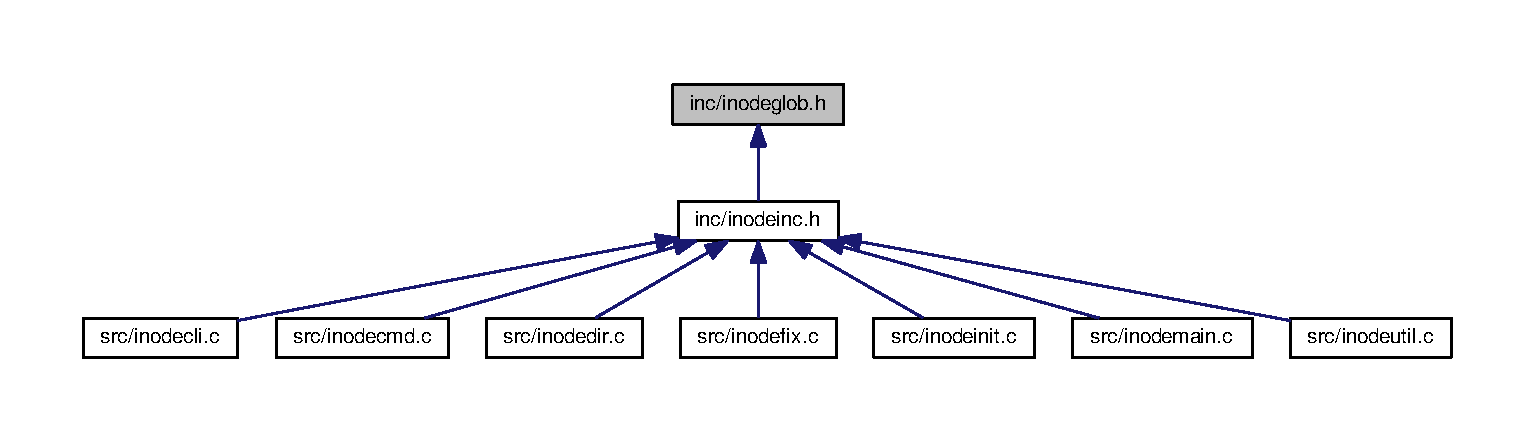
\includegraphics[width=350pt]{inodeglob_8h__dep__incl}
\end{center}
\end{figure}
\subsection*{Variables}
\begin{DoxyCompactItemize}
\item 
struct ext3\+\_\+group\+\_\+desc \hyperlink{inodeglob_8h_a8dd783d921ffbc92063db1fec0e3b449}{gd}
\item 
struct ext3\+\_\+super\+\_\+block \hyperlink{inodeglob_8h_a0a0039d94f74fad3d31338e4d26e61c3}{sb}
\item 
U\+I\+N\+T4 \hyperlink{inodeglob_8h_a579a32d3921440fafe49be9e94412fe7}{gu4\+Block\+Size}
\item 
U\+I\+N\+T4 \hyperlink{inodeglob_8h_a52ae935fec829526f7106c2567d29f86}{gu4\+File\+Des}
\item 
U\+I\+N\+T4 \hyperlink{inodeglob_8h_a04bbd984f1251e18176a1668605155a1}{gu4\+Corrupted\+Array} \mbox{[}\hyperlink{inodedef_8h_aa42e059eb1c65a67ae0a223128299a77}{M\+A\+X\+\_\+\+C\+O\+R\+R\+\_\+\+I\+N\+O\+D\+E\+S}\mbox{]}
\item 
I\+N\+T4 \hyperlink{inodeglob_8h_a3b1ca7f491ad5ac886b4bacb85dc9bf5}{gi4\+Array\+Index}
\item 
U\+I\+N\+T4 \hyperlink{inodeglob_8h_a901acbb8d2da8400086899838bba175d}{gu4\+Total\+Inodes}
\item 
U\+I\+N\+T1 $\ast$ \hyperlink{inodeglob_8h_a665f2580e620a4445d05edc1dcc276d5}{gp\+Inode\+Array}
\item 
U\+I\+N\+T4 \hyperlink{inodeglob_8h_a637920f896583ff8051c4a9d2c3d7a92}{gu4\+Root\+Data\+Block}
\end{DoxyCompactItemize}


\subsection{Variable Documentation}
\hypertarget{inodeglob_8h_a8dd783d921ffbc92063db1fec0e3b449}{\index{inodeglob.\+h@{inodeglob.\+h}!gd@{gd}}
\index{gd@{gd}!inodeglob.\+h@{inodeglob.\+h}}
\subsubsection[{gd}]{\setlength{\rightskip}{0pt plus 5cm}struct ext3\+\_\+group\+\_\+desc gd}}\label{inodeglob_8h_a8dd783d921ffbc92063db1fec0e3b449}
\hypertarget{inodeglob_8h_a3b1ca7f491ad5ac886b4bacb85dc9bf5}{\index{inodeglob.\+h@{inodeglob.\+h}!gi4\+Array\+Index@{gi4\+Array\+Index}}
\index{gi4\+Array\+Index@{gi4\+Array\+Index}!inodeglob.\+h@{inodeglob.\+h}}
\subsubsection[{gi4\+Array\+Index}]{\setlength{\rightskip}{0pt plus 5cm}I\+N\+T4 gi4\+Array\+Index}}\label{inodeglob_8h_a3b1ca7f491ad5ac886b4bacb85dc9bf5}
\hypertarget{inodeglob_8h_a665f2580e620a4445d05edc1dcc276d5}{\index{inodeglob.\+h@{inodeglob.\+h}!gp\+Inode\+Array@{gp\+Inode\+Array}}
\index{gp\+Inode\+Array@{gp\+Inode\+Array}!inodeglob.\+h@{inodeglob.\+h}}
\subsubsection[{gp\+Inode\+Array}]{\setlength{\rightskip}{0pt plus 5cm}U\+I\+N\+T1$\ast$ gp\+Inode\+Array}}\label{inodeglob_8h_a665f2580e620a4445d05edc1dcc276d5}
\hypertarget{inodeglob_8h_a579a32d3921440fafe49be9e94412fe7}{\index{inodeglob.\+h@{inodeglob.\+h}!gu4\+Block\+Size@{gu4\+Block\+Size}}
\index{gu4\+Block\+Size@{gu4\+Block\+Size}!inodeglob.\+h@{inodeglob.\+h}}
\subsubsection[{gu4\+Block\+Size}]{\setlength{\rightskip}{0pt plus 5cm}U\+I\+N\+T4 gu4\+Block\+Size}}\label{inodeglob_8h_a579a32d3921440fafe49be9e94412fe7}
\hypertarget{inodeglob_8h_a04bbd984f1251e18176a1668605155a1}{\index{inodeglob.\+h@{inodeglob.\+h}!gu4\+Corrupted\+Array@{gu4\+Corrupted\+Array}}
\index{gu4\+Corrupted\+Array@{gu4\+Corrupted\+Array}!inodeglob.\+h@{inodeglob.\+h}}
\subsubsection[{gu4\+Corrupted\+Array}]{\setlength{\rightskip}{0pt plus 5cm}U\+I\+N\+T4 gu4\+Corrupted\+Array\mbox{[}{\bf M\+A\+X\+\_\+\+C\+O\+R\+R\+\_\+\+I\+N\+O\+D\+E\+S}\mbox{]}}}\label{inodeglob_8h_a04bbd984f1251e18176a1668605155a1}
\hypertarget{inodeglob_8h_a52ae935fec829526f7106c2567d29f86}{\index{inodeglob.\+h@{inodeglob.\+h}!gu4\+File\+Des@{gu4\+File\+Des}}
\index{gu4\+File\+Des@{gu4\+File\+Des}!inodeglob.\+h@{inodeglob.\+h}}
\subsubsection[{gu4\+File\+Des}]{\setlength{\rightskip}{0pt plus 5cm}U\+I\+N\+T4 gu4\+File\+Des}}\label{inodeglob_8h_a52ae935fec829526f7106c2567d29f86}
\hypertarget{inodeglob_8h_a637920f896583ff8051c4a9d2c3d7a92}{\index{inodeglob.\+h@{inodeglob.\+h}!gu4\+Root\+Data\+Block@{gu4\+Root\+Data\+Block}}
\index{gu4\+Root\+Data\+Block@{gu4\+Root\+Data\+Block}!inodeglob.\+h@{inodeglob.\+h}}
\subsubsection[{gu4\+Root\+Data\+Block}]{\setlength{\rightskip}{0pt plus 5cm}U\+I\+N\+T4 gu4\+Root\+Data\+Block}}\label{inodeglob_8h_a637920f896583ff8051c4a9d2c3d7a92}
\hypertarget{inodeglob_8h_a901acbb8d2da8400086899838bba175d}{\index{inodeglob.\+h@{inodeglob.\+h}!gu4\+Total\+Inodes@{gu4\+Total\+Inodes}}
\index{gu4\+Total\+Inodes@{gu4\+Total\+Inodes}!inodeglob.\+h@{inodeglob.\+h}}
\subsubsection[{gu4\+Total\+Inodes}]{\setlength{\rightskip}{0pt plus 5cm}U\+I\+N\+T4 gu4\+Total\+Inodes}}\label{inodeglob_8h_a901acbb8d2da8400086899838bba175d}
\hypertarget{inodeglob_8h_a0a0039d94f74fad3d31338e4d26e61c3}{\index{inodeglob.\+h@{inodeglob.\+h}!sb@{sb}}
\index{sb@{sb}!inodeglob.\+h@{inodeglob.\+h}}
\subsubsection[{sb}]{\setlength{\rightskip}{0pt plus 5cm}struct ext3\+\_\+super\+\_\+block sb}}\label{inodeglob_8h_a0a0039d94f74fad3d31338e4d26e61c3}

\hypertarget{inodeinc_8h}{\section{inc/inodeinc.h File Reference}
\label{inodeinc_8h}\index{inc/inodeinc.\+h@{inc/inodeinc.\+h}}
}
{\ttfamily \#include \char`\"{}cmninc.\+h\char`\"{}}\\*
{\ttfamily \#include \char`\"{}inodetdfs.\+h\char`\"{}}\\*
{\ttfamily \#include \char`\"{}inodeproto.\+h\char`\"{}}\\*
{\ttfamily \#include \char`\"{}inodedef.\+h\char`\"{}}\\*
{\ttfamily \#include \char`\"{}inodeglob.\+h\char`\"{}}\\*
{\ttfamily \#include $<$sys/time.\+h$>$}\\*
Include dependency graph for inodeinc.\+h\+:\nopagebreak
\begin{figure}[H]
\begin{center}
\leavevmode
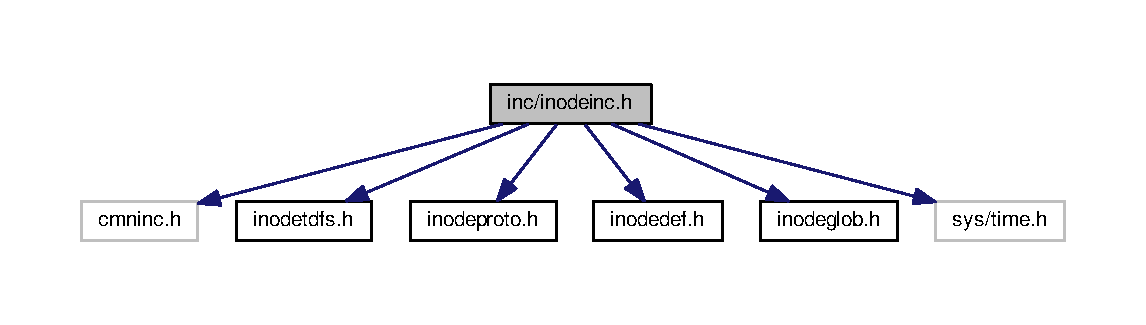
\includegraphics[width=350pt]{inodeinc_8h__incl}
\end{center}
\end{figure}
This graph shows which files directly or indirectly include this file\+:\nopagebreak
\begin{figure}[H]
\begin{center}
\leavevmode
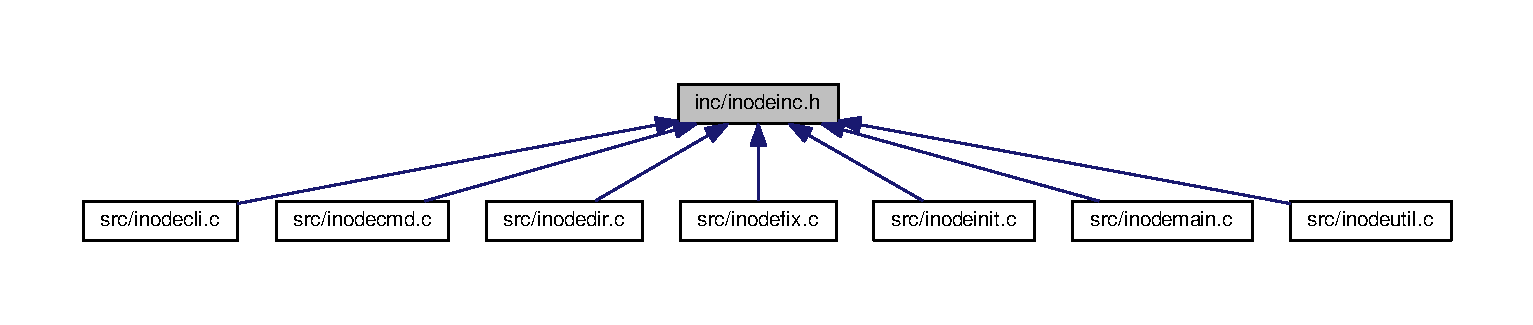
\includegraphics[width=350pt]{inodeinc_8h__dep__incl}
\end{center}
\end{figure}

\hypertarget{inodeproto_8h}{\section{inc/inodeproto.h File Reference}
\label{inodeproto_8h}\index{inc/inodeproto.\+h@{inc/inodeproto.\+h}}
}
This graph shows which files directly or indirectly include this file\+:\nopagebreak
\begin{figure}[H]
\begin{center}
\leavevmode
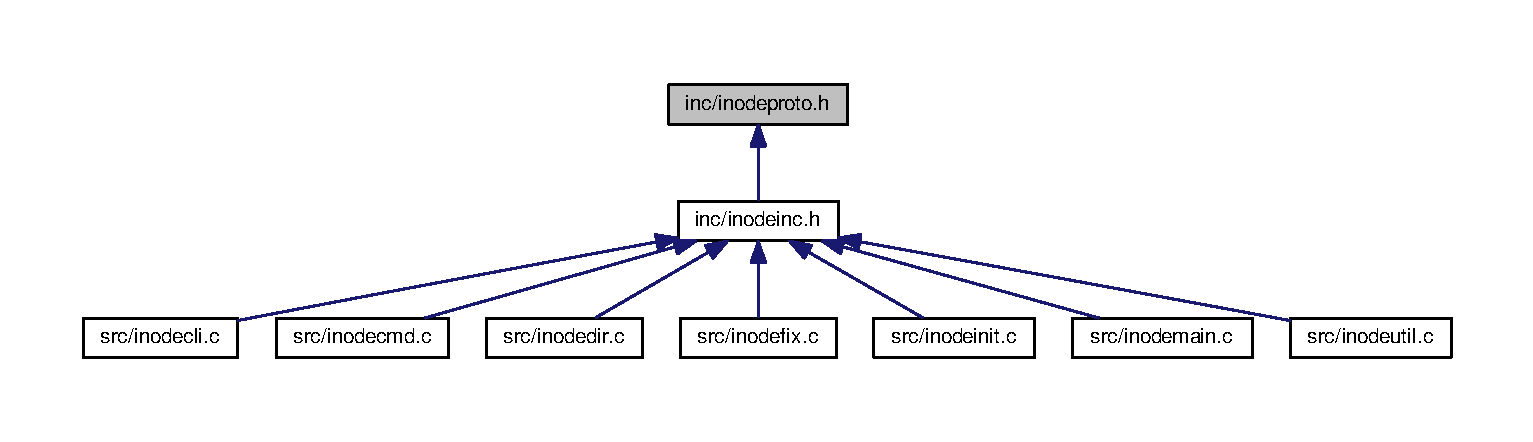
\includegraphics[width=350pt]{inodeproto_8h__dep__incl}
\end{center}
\end{figure}
\subsection*{Functions}
\begin{DoxyCompactItemize}
\item 
I\+N\+T4 \hyperlink{inodeproto_8h_a6474c5fd62b8ca4f7745428690849175}{Inode\+Util\+Print\+Children} (U\+I\+N\+T4 u4\+Block\+No, U\+I\+N\+T4 u4\+Level)
\item 
I\+N\+T4 \hyperlink{inodeproto_8h_af3bd13d59e79a9c574862e0a42ac1ac2}{Inode\+Util\+Print\+Tree} (U\+I\+N\+T4 u4\+Inode\+No, U\+I\+N\+T4 u4\+Level)
\item 
V\+O\+I\+D \hyperlink{inodeproto_8h_af56b9ef4fbba04cbcdc61dfcda95c33b}{Inode\+Util\+Dump\+Dir\+Entry} (struct ext3\+\_\+dir\+\_\+entry\+\_\+2 $\ast$p\+Dir\+Entry, \hyperlink{inodetdfs_8h_a408cefd7ee29ff67ed7fefab9393affa}{t\+File\+Filter} Filter, U\+I\+N\+T4 u4\+Level)
\item 
V\+O\+I\+D \hyperlink{inodeproto_8h_a02fc70420f966503493dcee4f275951c}{Inode\+Util\+Dump\+Inode} (struct ext3\+\_\+inode $\ast$p\+Inode)
\item 
V\+O\+I\+D \hyperlink{inodeproto_8h_a91e76cac49f4444a82a74a2fa004011d}{Inode\+Util\+Dump\+Data\+Block\+Raw} (C\+H\+A\+R $\ast$p\+Buffer)
\item 
I\+N\+T4 \hyperlink{inodeproto_8h_a6867770228931c846eac7d67ffc582a0}{Inode\+Util\+Read\+Inode} (U\+I\+N\+T4 u4\+Inode, struct ext3\+\_\+inode $\ast$p\+New\+Inode)
\item 
I\+N\+T4 \hyperlink{inodeproto_8h_a3add91b54cfb3e27f802ac8ab1b9ceb4}{Inode\+Util\+Read\+Data\+Offset} (U\+I\+N\+T8 u8\+Offset, V\+O\+I\+D $\ast$p\+Buffer, U\+I\+N\+T4 u4\+Size)
\item 
I\+N\+T4 \hyperlink{inodeproto_8h_a13b5c799edb137a494ad497145f59a56}{Inode\+Util\+Read\+Data\+Block} (U\+I\+N\+T4 u4\+Block\+No, U\+I\+N\+T2 u2\+Start\+Pos, V\+O\+I\+D $\ast$p\+Buffer, U\+I\+N\+T4 u4\+Size)
\item 
I\+N\+T4 \hyperlink{inodeproto_8h_a9671fcb9023997872ade29c0241b0cab}{Inode\+Util\+Write\+Data\+Offset} (U\+I\+N\+T8 u8\+Offset, V\+O\+I\+D $\ast$p\+Buffer, U\+I\+N\+T4 u4\+Size)
\item 
I\+N\+T4 \hyperlink{inodeproto_8h_af4e29989b8cc9424603a4825af3491a0}{Inode\+Util\+Write\+Data\+Block} (U\+I\+N\+T4 u4\+Block\+No, U\+I\+N\+T2 u2\+Start\+Pos, V\+O\+I\+D $\ast$p\+Buffer, U\+I\+N\+T4 u4\+Size)
\item 
I\+N\+T4 \hyperlink{inodeproto_8h_a0bb419219a634fdfbb0e32df8fd4f937}{Inode\+Util\+Print\+Dir\+Data\+Block} (U\+I\+N\+T4 u4\+Block\+No)
\item 
I\+N\+T4 \hyperlink{inodeproto_8h_a45685e5c715aa741d487eae77c1083ae}{Inode\+Util\+Print\+Inode} (U\+I\+N\+T4 u4\+Inode\+No)
\item 
I\+N\+T4 \hyperlink{inodeproto_8h_a07685cf3d25b03c9e975af7d0f22ca81}{Inode\+Util\+Get\+Inode\+Offset} (U\+I\+N\+T4 u4\+Inode\+No, U\+I\+N\+T8 $\ast$u8\+Offset)
\item 
I\+N\+T4 \hyperlink{inodeproto_8h_a091aeb9997faf9dae00a698c470439e9}{Inode\+Util\+Check\+Corrupted\+Inode} (U\+I\+N\+T4 u4\+Inode\+No)
\item 
I\+N\+T4 \hyperlink{inodeproto_8h_ae4aa54c12d8e18c272feab11068a1cfb}{Inode\+Util\+Corrupt\+And\+Recover} (U\+I\+N\+T4 u4\+Inode\+No, U\+I\+N\+T4 u4\+Cmd)
\item 
I\+N\+T1 \hyperlink{inodeproto_8h_a63b7552b4e10719ea82758cb689850a8}{Inode\+Util\+Is\+Free\+Inode} (struct ext3\+\_\+inode $\ast$p\+Inode)
\item 
I\+N\+T4 \hyperlink{inodeproto_8h_a9513ab1ee8f7fcc872a1f5c14af8a985}{Inode\+Dir\+Read\+Record} (C\+H\+A\+R $\ast$p\+Entries, U\+I\+N\+T4 u4\+Start\+Pos, struct ext3\+\_\+dir\+\_\+entry\+\_\+2 $\ast$p\+Dir\+Entry)
\item 
I\+N\+T4 \hyperlink{inodeproto_8h_a948215ffdfa5ea0b20495807546f1e09}{Inode\+Dir\+Verify\+Dir\+Record} (C\+H\+A\+R $\ast$p\+Entries, struct ext3\+\_\+dir\+\_\+entry\+\_\+2 $\ast$p\+Dir\+Entry, U\+I\+N\+T2 u4\+Start\+Pos)
\item 
I\+N\+T4 \hyperlink{inodeproto_8h_a648f1f0adeeb821396ff675be7ce3a0a}{Inode\+Dir\+Validate\+Inode} (U\+I\+N\+T4 u4\+Inode\+No, U\+I\+N\+T4 u4\+Block\+No)
\item 
I\+N\+T4 \hyperlink{inodeproto_8h_a90a015688692be14fcbf9ad6f52b24b2}{Inode\+Dir\+Validate\+Data\+Block} (C\+H\+A\+R $\ast$p\+Entries)
\item 
I\+N\+T4 \hyperlink{inodeproto_8h_a89c0632678345a3ec36ec25c31872df4}{Inode\+Dir\+Change\+Parent\+Entry} (struct ext3\+\_\+dir\+\_\+entry\+\_\+2 $\ast$p\+Dir\+Entry, U\+I\+N\+T4 u4\+Block\+No)
\item 
I\+N\+T4 \hyperlink{inodeproto_8h_accaeb48b7288571f8cb5db824b02cb9d}{Inode\+Dir\+Add\+Child\+Entry} (struct ext3\+\_\+dir\+\_\+entry\+\_\+2 $\ast$p\+Dir\+Entry, U\+I\+N\+T4 u4\+Block\+No)
\item 
I\+N\+T4 \hyperlink{inodeproto_8h_a0cf855704a34cb63b52487e75b12052c}{Inode\+Fix\+Execute} ()
\item 
I\+N\+T4 \hyperlink{inodeproto_8h_adbd08c2df1e429581a73b0ffd6108cb6}{Inode\+Fix\+Root\+Data\+Block\+Ptr} (struct ext3\+\_\+inode $\ast$p\+Inode)
\end{DoxyCompactItemize}


\subsection{Function Documentation}
\hypertarget{inodeproto_8h_accaeb48b7288571f8cb5db824b02cb9d}{\index{inodeproto.\+h@{inodeproto.\+h}!Inode\+Dir\+Add\+Child\+Entry@{Inode\+Dir\+Add\+Child\+Entry}}
\index{Inode\+Dir\+Add\+Child\+Entry@{Inode\+Dir\+Add\+Child\+Entry}!inodeproto.\+h@{inodeproto.\+h}}
\subsubsection[{Inode\+Dir\+Add\+Child\+Entry}]{\setlength{\rightskip}{0pt plus 5cm}I\+N\+T4 Inode\+Dir\+Add\+Child\+Entry (
\begin{DoxyParamCaption}
\item[{struct ext3\+\_\+dir\+\_\+entry\+\_\+2 $\ast$}]{p\+New\+Child, }
\item[{U\+I\+N\+T4}]{u4\+Block\+No}
\end{DoxyParamCaption}
)}}\label{inodeproto_8h_accaeb48b7288571f8cb5db824b02cb9d}


 Function Name \+: Inode\+Dir\+Add\+Child\+Entry

Author \+: Anusha Seshadri

Description \+: This Function is used to add a child entry to a directory inode. The new entry would be appended at the end of the last entry.

Input \+: p\+Dir\+Entry -\/ new child entry u4\+Block\+No -\/ the directory data block where the child entry needs to be changed Output \+: None

Returns \+: I\+N\+O\+D\+E\+\_\+\+S\+U\+C\+C\+E\+S\+S, if the child entry is addded successfully I\+N\+O\+D\+E\+\_\+\+F\+A\+I\+L\+U\+R\+E otherwise 

Here is the call graph for this function\+:\nopagebreak
\begin{figure}[H]
\begin{center}
\leavevmode
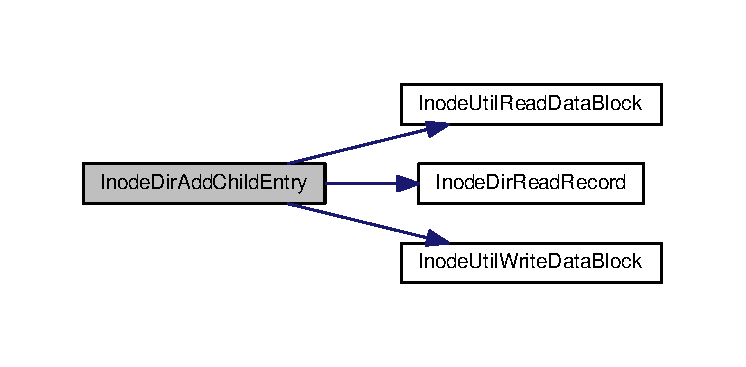
\includegraphics[width=350pt]{inodeproto_8h_accaeb48b7288571f8cb5db824b02cb9d_cgraph}
\end{center}
\end{figure}


\hypertarget{inodeproto_8h_a89c0632678345a3ec36ec25c31872df4}{\index{inodeproto.\+h@{inodeproto.\+h}!Inode\+Dir\+Change\+Parent\+Entry@{Inode\+Dir\+Change\+Parent\+Entry}}
\index{Inode\+Dir\+Change\+Parent\+Entry@{Inode\+Dir\+Change\+Parent\+Entry}!inodeproto.\+h@{inodeproto.\+h}}
\subsubsection[{Inode\+Dir\+Change\+Parent\+Entry}]{\setlength{\rightskip}{0pt plus 5cm}I\+N\+T4 Inode\+Dir\+Change\+Parent\+Entry (
\begin{DoxyParamCaption}
\item[{struct ext3\+\_\+dir\+\_\+entry\+\_\+2 $\ast$}]{p\+Dir\+Entry, }
\item[{U\+I\+N\+T4}]{u4\+Block\+No}
\end{DoxyParamCaption}
)}}\label{inodeproto_8h_a89c0632678345a3ec36ec25c31872df4}


 Function Name \+: Inode\+Dir\+Change\+Parent\+Entry

Author \+: Anusha Seshadri

Description \+: This Function is used to change the parent directory entry of a directory inode.

Input \+: p\+Dir\+Entry -\/ new parent entry u4\+Block\+No -\/ the directory data block where the parent entry needs to be changed Output \+: None

Returns \+: I\+N\+O\+D\+E\+\_\+\+S\+U\+C\+C\+E\+S\+S, if the parent is changed successfully I\+N\+O\+D\+E\+\_\+\+F\+A\+I\+L\+U\+R\+E otherwise 

Here is the call graph for this function\+:\nopagebreak
\begin{figure}[H]
\begin{center}
\leavevmode
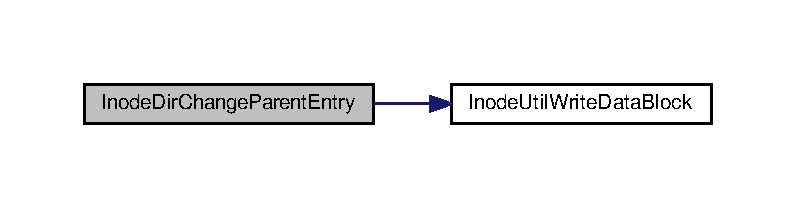
\includegraphics[width=350pt]{inodeproto_8h_a89c0632678345a3ec36ec25c31872df4_cgraph}
\end{center}
\end{figure}


\hypertarget{inodeproto_8h_a9513ab1ee8f7fcc872a1f5c14af8a985}{\index{inodeproto.\+h@{inodeproto.\+h}!Inode\+Dir\+Read\+Record@{Inode\+Dir\+Read\+Record}}
\index{Inode\+Dir\+Read\+Record@{Inode\+Dir\+Read\+Record}!inodeproto.\+h@{inodeproto.\+h}}
\subsubsection[{Inode\+Dir\+Read\+Record}]{\setlength{\rightskip}{0pt plus 5cm}I\+N\+T4 Inode\+Dir\+Read\+Record (
\begin{DoxyParamCaption}
\item[{C\+H\+A\+R $\ast$}]{p\+Entries, }
\item[{U\+I\+N\+T4}]{u4\+Start\+Pos, }
\item[{struct ext3\+\_\+dir\+\_\+entry\+\_\+2 $\ast$}]{p\+Dir\+Entry}
\end{DoxyParamCaption}
)}}\label{inodeproto_8h_a9513ab1ee8f7fcc872a1f5c14af8a985}


 Function Name \+: Inode\+Dir\+Read\+Record

Author \+: Naveen Raj Selvaraj

Description \+: This Function is used to read a directory entry from the data block of a directory inode.

Input \+: p\+Entries -\/ Buffer containing the contents of the data block u4\+Start\+Pos -\/ Offset to start reading

Output \+: p\+Dir\+Entry -\/ the directory entry read from the block

Returns \+: I\+N\+O\+D\+E\+\_\+\+S\+U\+C\+C\+E\+S\+S, if the entry is read successfully I\+N\+O\+D\+E\+\_\+\+F\+A\+I\+L\+U\+R\+E otherwise \hypertarget{inodeproto_8h_a90a015688692be14fcbf9ad6f52b24b2}{\index{inodeproto.\+h@{inodeproto.\+h}!Inode\+Dir\+Validate\+Data\+Block@{Inode\+Dir\+Validate\+Data\+Block}}
\index{Inode\+Dir\+Validate\+Data\+Block@{Inode\+Dir\+Validate\+Data\+Block}!inodeproto.\+h@{inodeproto.\+h}}
\subsubsection[{Inode\+Dir\+Validate\+Data\+Block}]{\setlength{\rightskip}{0pt plus 5cm}I\+N\+T4 Inode\+Dir\+Validate\+Data\+Block (
\begin{DoxyParamCaption}
\item[{C\+H\+A\+R $\ast$}]{p\+Entries}
\end{DoxyParamCaption}
)}}\label{inodeproto_8h_a90a015688692be14fcbf9ad6f52b24b2}


 Function Name \+: Inode\+Dir\+Validate\+Data\+Block

Author \+: Naveen Raj Selvaraj

Description \+: This Function is used to check if a data block is a directory data block or not. If the data block contains directory entries, then it is a valid directory data block.

Input \+: p\+Entries -\/ Buffer containing the contents of the data block Output \+: None

Returns \+: I\+N\+O\+D\+E\+\_\+\+S\+U\+C\+C\+E\+S\+S, if the data block is a valid directory data block I\+N\+O\+D\+E\+\_\+\+F\+A\+I\+L\+U\+R\+E otherwise \hypertarget{inodeproto_8h_a648f1f0adeeb821396ff675be7ce3a0a}{\index{inodeproto.\+h@{inodeproto.\+h}!Inode\+Dir\+Validate\+Inode@{Inode\+Dir\+Validate\+Inode}}
\index{Inode\+Dir\+Validate\+Inode@{Inode\+Dir\+Validate\+Inode}!inodeproto.\+h@{inodeproto.\+h}}
\subsubsection[{Inode\+Dir\+Validate\+Inode}]{\setlength{\rightskip}{0pt plus 5cm}I\+N\+T4 Inode\+Dir\+Validate\+Inode (
\begin{DoxyParamCaption}
\item[{U\+I\+N\+T4}]{u4\+Inode\+No, }
\item[{U\+I\+N\+T4}]{u4\+Block\+No}
\end{DoxyParamCaption}
)}}\label{inodeproto_8h_a648f1f0adeeb821396ff675be7ce3a0a}


 Function Name \+: Inode\+Dir\+Validate\+Inode

Author \+: Naveen Raj Selvaraj

Description \+: This Function is used to validate a directory inode. A directory inode is valid if the data block pointer points to the actual data block of inode. If the data block pointer is corrupted, then the directory inode is invalid.

Input \+: u4\+Inode\+No -\/ Directory Inode number u4\+Block\+No -\/ data block pointed by the inode's first direct block pointer Output \+: None

Returns \+: I\+N\+O\+D\+E\+\_\+\+S\+U\+C\+C\+E\+S\+S, if the inode is a valid directory inode I\+N\+O\+D\+E\+\_\+\+F\+A\+I\+L\+U\+R\+E otherwise 

Here is the call graph for this function\+:\nopagebreak
\begin{figure}[H]
\begin{center}
\leavevmode
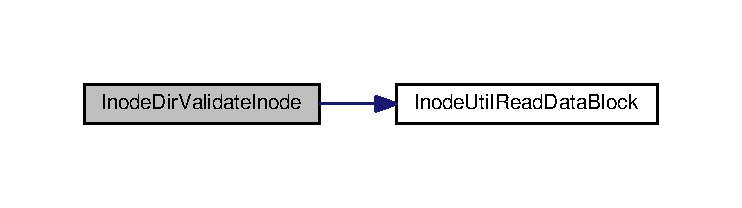
\includegraphics[width=350pt]{inodeproto_8h_a648f1f0adeeb821396ff675be7ce3a0a_cgraph}
\end{center}
\end{figure}


\hypertarget{inodeproto_8h_a948215ffdfa5ea0b20495807546f1e09}{\index{inodeproto.\+h@{inodeproto.\+h}!Inode\+Dir\+Verify\+Dir\+Record@{Inode\+Dir\+Verify\+Dir\+Record}}
\index{Inode\+Dir\+Verify\+Dir\+Record@{Inode\+Dir\+Verify\+Dir\+Record}!inodeproto.\+h@{inodeproto.\+h}}
\subsubsection[{Inode\+Dir\+Verify\+Dir\+Record}]{\setlength{\rightskip}{0pt plus 5cm}I\+N\+T4 Inode\+Dir\+Verify\+Dir\+Record (
\begin{DoxyParamCaption}
\item[{C\+H\+A\+R $\ast$}]{p\+Entries, }
\item[{struct ext3\+\_\+dir\+\_\+entry\+\_\+2 $\ast$}]{p\+Dir\+Entry, }
\item[{U\+I\+N\+T2}]{u4\+Start\+Pos}
\end{DoxyParamCaption}
)}}\label{inodeproto_8h_a948215ffdfa5ea0b20495807546f1e09}
\hypertarget{inodeproto_8h_a0cf855704a34cb63b52487e75b12052c}{\index{inodeproto.\+h@{inodeproto.\+h}!Inode\+Fix\+Execute@{Inode\+Fix\+Execute}}
\index{Inode\+Fix\+Execute@{Inode\+Fix\+Execute}!inodeproto.\+h@{inodeproto.\+h}}
\subsubsection[{Inode\+Fix\+Execute}]{\setlength{\rightskip}{0pt plus 5cm}I\+N\+T4 Inode\+Fix\+Execute (
\begin{DoxyParamCaption}
{}
\end{DoxyParamCaption}
)}}\label{inodeproto_8h_a0cf855704a34cb63b52487e75b12052c}


 Function Name \+: Inode\+Fix\+Execute

Description \+: This Function is used to recover the corrupted directories children directories. Please refer the documentation for the recovery algorithm.

Input \+: None

Output \+: None

Returns \+: I\+N\+O\+D\+E\+\_\+\+S\+U\+C\+C\+E\+S\+S, on successful recovery I\+N\+O\+D\+E\+\_\+\+F\+A\+I\+L\+U\+R\+E otherwise 

Here is the call graph for this function\+:\nopagebreak
\begin{figure}[H]
\begin{center}
\leavevmode
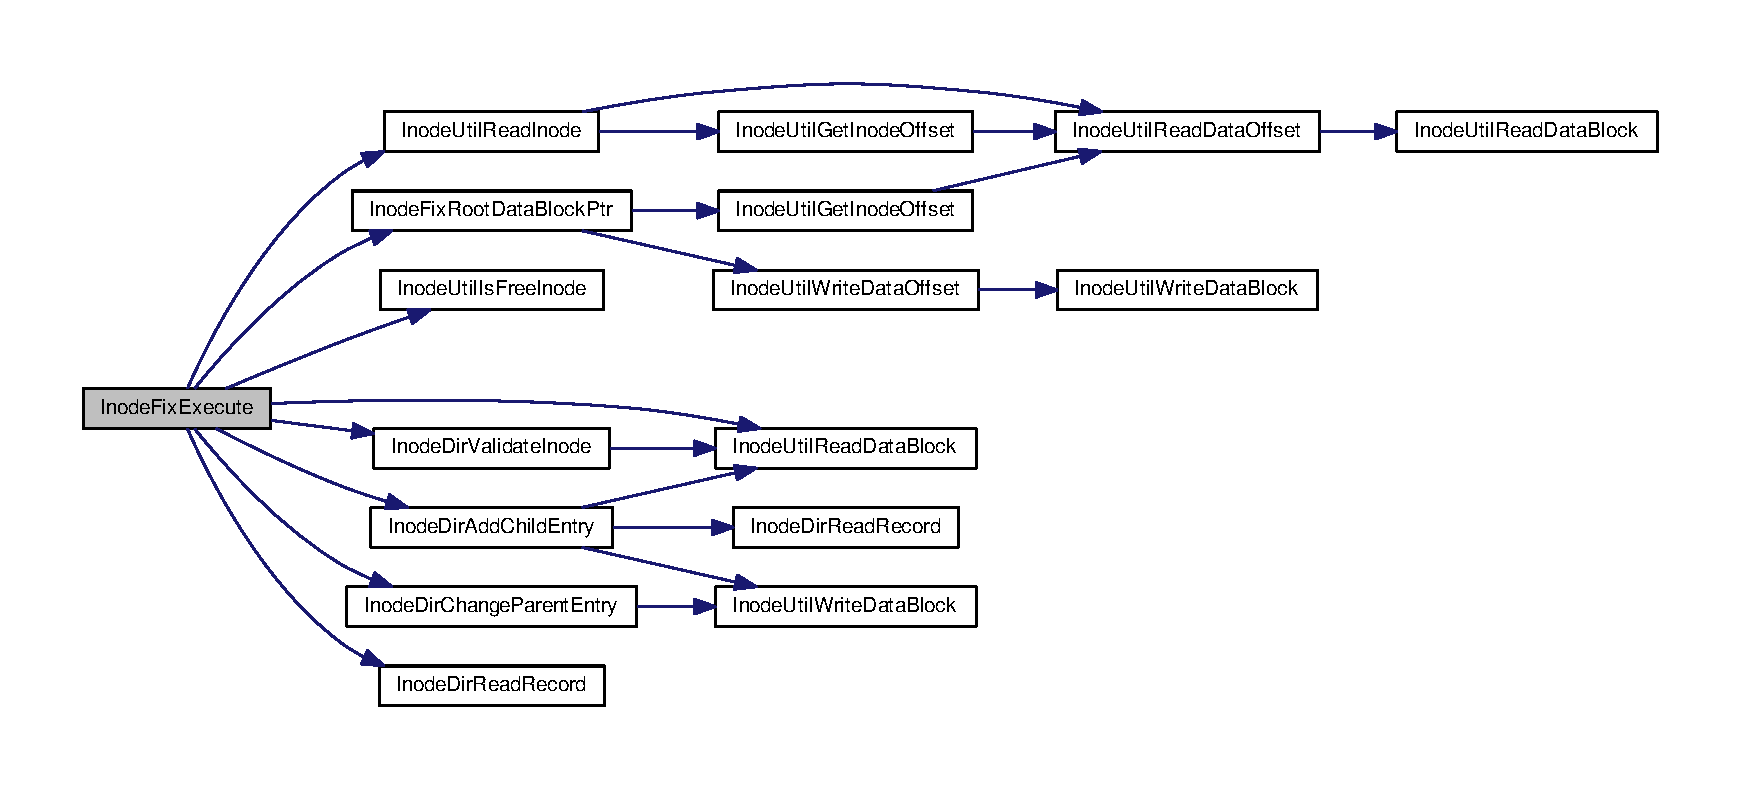
\includegraphics[width=350pt]{inodeproto_8h_a0cf855704a34cb63b52487e75b12052c_cgraph}
\end{center}
\end{figure}


\hypertarget{inodeproto_8h_adbd08c2df1e429581a73b0ffd6108cb6}{\index{inodeproto.\+h@{inodeproto.\+h}!Inode\+Fix\+Root\+Data\+Block\+Ptr@{Inode\+Fix\+Root\+Data\+Block\+Ptr}}
\index{Inode\+Fix\+Root\+Data\+Block\+Ptr@{Inode\+Fix\+Root\+Data\+Block\+Ptr}!inodeproto.\+h@{inodeproto.\+h}}
\subsubsection[{Inode\+Fix\+Root\+Data\+Block\+Ptr}]{\setlength{\rightskip}{0pt plus 5cm}I\+N\+T4 Inode\+Fix\+Root\+Data\+Block\+Ptr (
\begin{DoxyParamCaption}
\item[{struct ext3\+\_\+inode $\ast$}]{p\+Inode}
\end{DoxyParamCaption}
)}}\label{inodeproto_8h_adbd08c2df1e429581a73b0ffd6108cb6}


 Function Name \+: Inode\+Fix\+Root\+Data\+Block\+Ptr

Description \+: This Function is used to fix the root inode's data block pointer if it is corrupted.

Input \+: p\+Inode -\/ Root Inode structure

Output \+: None

Returns \+: I\+N\+O\+D\+E\+\_\+\+S\+U\+C\+C\+E\+S\+S, if the data block pointer is fixed I\+N\+O\+D\+E\+\_\+\+F\+A\+I\+L\+U\+R\+E otherwise 

Here is the call graph for this function\+:\nopagebreak
\begin{figure}[H]
\begin{center}
\leavevmode
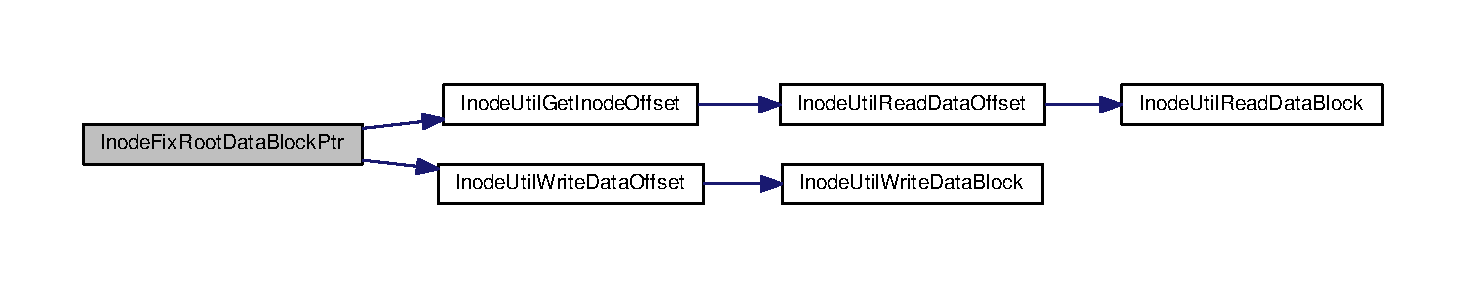
\includegraphics[width=350pt]{inodeproto_8h_adbd08c2df1e429581a73b0ffd6108cb6_cgraph}
\end{center}
\end{figure}


\hypertarget{inodeproto_8h_a091aeb9997faf9dae00a698c470439e9}{\index{inodeproto.\+h@{inodeproto.\+h}!Inode\+Util\+Check\+Corrupted\+Inode@{Inode\+Util\+Check\+Corrupted\+Inode}}
\index{Inode\+Util\+Check\+Corrupted\+Inode@{Inode\+Util\+Check\+Corrupted\+Inode}!inodeproto.\+h@{inodeproto.\+h}}
\subsubsection[{Inode\+Util\+Check\+Corrupted\+Inode}]{\setlength{\rightskip}{0pt plus 5cm}I\+N\+T4 Inode\+Util\+Check\+Corrupted\+Inode (
\begin{DoxyParamCaption}
\item[{U\+I\+N\+T4}]{u4\+Inode\+No}
\end{DoxyParamCaption}
)}}\label{inodeproto_8h_a091aeb9997faf9dae00a698c470439e9}


 Function Name \+: Inode\+Util\+Check\+Corrupted\+Inode

Author \+: Anusha Seshadri

Description \+: This Function is used during manual corruption to check whether the inode is already corrupted manually or not.

Input \+: u4\+Inode\+No -\/ Inode number

Output \+: None

Returns \+: array index in the corrupted array, if the inode is corrupted I\+N\+O\+D\+E\+\_\+\+F\+A\+I\+L\+U\+R\+E if it is not corrupted already \hypertarget{inodeproto_8h_ae4aa54c12d8e18c272feab11068a1cfb}{\index{inodeproto.\+h@{inodeproto.\+h}!Inode\+Util\+Corrupt\+And\+Recover@{Inode\+Util\+Corrupt\+And\+Recover}}
\index{Inode\+Util\+Corrupt\+And\+Recover@{Inode\+Util\+Corrupt\+And\+Recover}!inodeproto.\+h@{inodeproto.\+h}}
\subsubsection[{Inode\+Util\+Corrupt\+And\+Recover}]{\setlength{\rightskip}{0pt plus 5cm}I\+N\+T4 Inode\+Util\+Corrupt\+And\+Recover (
\begin{DoxyParamCaption}
\item[{U\+I\+N\+T4}]{u4\+Inode\+No, }
\item[{U\+I\+N\+T4}]{u4\+Cmd}
\end{DoxyParamCaption}
)}}\label{inodeproto_8h_ae4aa54c12d8e18c272feab11068a1cfb}


 Function Name \+: Inode\+Util\+Corrupt\+And\+Recover

Author \+: Anusha Seshadri

Description \+: This Function is used to manually corrupt and fix an inode.

Input \+: u4\+Inode\+No -\/ Inode to corrupt/fix u4\+Cmd -\/ I\+N\+O\+D\+E\+\_\+\+C\+O\+R\+R\+U\+P\+T to corrupt I\+N\+O\+D\+E\+\_\+\+F\+I\+X to fix Output \+: None

Returns \+: I\+N\+O\+D\+E\+\_\+\+S\+U\+C\+C\+E\+S\+S I\+N\+O\+D\+E\+\_\+\+F\+A\+I\+L\+U\+R\+E 

Here is the call graph for this function\+:\nopagebreak
\begin{figure}[H]
\begin{center}
\leavevmode
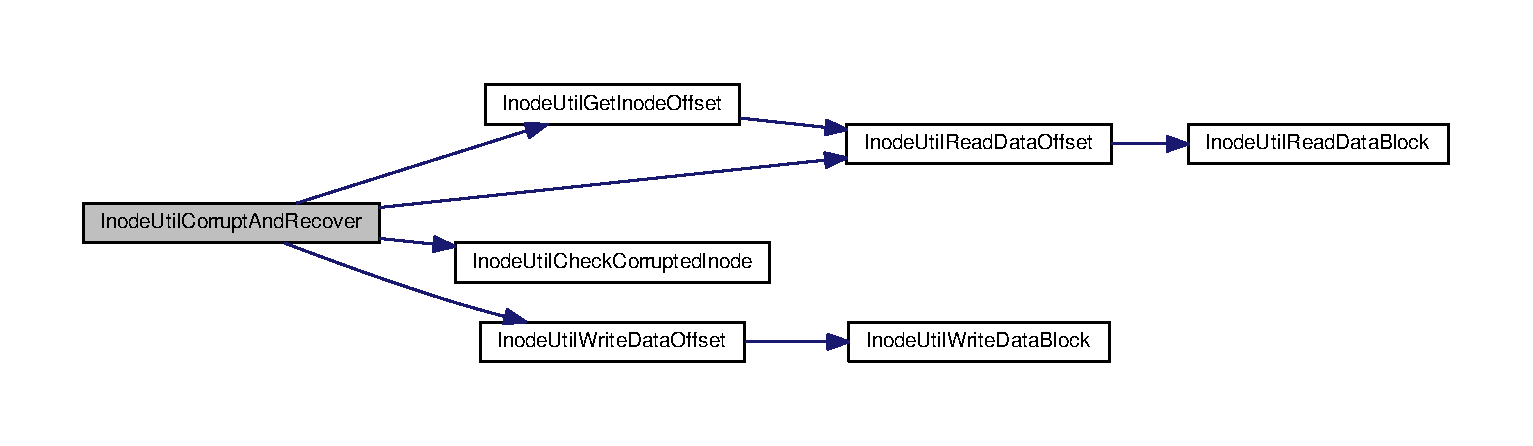
\includegraphics[width=350pt]{inodeproto_8h_ae4aa54c12d8e18c272feab11068a1cfb_cgraph}
\end{center}
\end{figure}


\hypertarget{inodeproto_8h_a91e76cac49f4444a82a74a2fa004011d}{\index{inodeproto.\+h@{inodeproto.\+h}!Inode\+Util\+Dump\+Data\+Block\+Raw@{Inode\+Util\+Dump\+Data\+Block\+Raw}}
\index{Inode\+Util\+Dump\+Data\+Block\+Raw@{Inode\+Util\+Dump\+Data\+Block\+Raw}!inodeproto.\+h@{inodeproto.\+h}}
\subsubsection[{Inode\+Util\+Dump\+Data\+Block\+Raw}]{\setlength{\rightskip}{0pt plus 5cm}V\+O\+I\+D Inode\+Util\+Dump\+Data\+Block\+Raw (
\begin{DoxyParamCaption}
\item[{C\+H\+A\+R $\ast$}]{p\+Buffer}
\end{DoxyParamCaption}
)}}\label{inodeproto_8h_a91e76cac49f4444a82a74a2fa004011d}


 Function Name \+: Inode\+Util\+Dump\+Data\+Block\+Raw

Author \+: Naveen Raj Selvaraj

Description \+: This Function is used to print the content of a block in H\+E\+X

Input \+: p\+Buffer -\/ buffer containing the data block contents

Output \+: None

Returns \+: None \hypertarget{inodeproto_8h_af56b9ef4fbba04cbcdc61dfcda95c33b}{\index{inodeproto.\+h@{inodeproto.\+h}!Inode\+Util\+Dump\+Dir\+Entry@{Inode\+Util\+Dump\+Dir\+Entry}}
\index{Inode\+Util\+Dump\+Dir\+Entry@{Inode\+Util\+Dump\+Dir\+Entry}!inodeproto.\+h@{inodeproto.\+h}}
\subsubsection[{Inode\+Util\+Dump\+Dir\+Entry}]{\setlength{\rightskip}{0pt plus 5cm}V\+O\+I\+D Inode\+Util\+Dump\+Dir\+Entry (
\begin{DoxyParamCaption}
\item[{struct ext3\+\_\+dir\+\_\+entry\+\_\+2 $\ast$}]{p\+Dir\+Entry, }
\item[{{\bf t\+File\+Filter}}]{Filter, }
\item[{U\+I\+N\+T4}]{u4\+Level}
\end{DoxyParamCaption}
)}}\label{inodeproto_8h_af56b9ef4fbba04cbcdc61dfcda95c33b}


 Function Name \+: Inode\+Util\+Dump\+Dir\+Entry

Author \+: Naveen Raj Selvaraj

Description \+: This Function is used to print a directory entry.

Input \+: p\+Dir\+Entry -\/ pointer to the directory entry to print Filter -\/ F\+I\+L\+E\+\_\+\+T\+Y\+P\+E\+\_\+\+D\+I\+R\+S -\/ print only directories F\+I\+L\+E\+\_\+\+T\+Y\+P\+E\+\_\+\+F\+I\+L\+E\+S -\/ print directories and files F\+I\+L\+E\+\_\+\+T\+Y\+P\+E\+\_\+\+A\+L\+L -\/ print everything including . and .. entries u4\+Level -\/ depth of this entry in the tree (used to format the output) Output \+: None

Returns \+: None \hypertarget{inodeproto_8h_a02fc70420f966503493dcee4f275951c}{\index{inodeproto.\+h@{inodeproto.\+h}!Inode\+Util\+Dump\+Inode@{Inode\+Util\+Dump\+Inode}}
\index{Inode\+Util\+Dump\+Inode@{Inode\+Util\+Dump\+Inode}!inodeproto.\+h@{inodeproto.\+h}}
\subsubsection[{Inode\+Util\+Dump\+Inode}]{\setlength{\rightskip}{0pt plus 5cm}V\+O\+I\+D Inode\+Util\+Dump\+Inode (
\begin{DoxyParamCaption}
\item[{struct ext3\+\_\+inode $\ast$}]{p\+Inode}
\end{DoxyParamCaption}
)}}\label{inodeproto_8h_a02fc70420f966503493dcee4f275951c}


 Function Name \+: Inode\+Util\+Dump\+Inode

Author \+: Naveen Raj Selvaraj

Description \+: This Function is used to print the ext3\+\_\+inode structure

Input \+: p\+Inode -\/ pointer to the inode structure

Output \+: None

Returns \+: None \hypertarget{inodeproto_8h_a07685cf3d25b03c9e975af7d0f22ca81}{\index{inodeproto.\+h@{inodeproto.\+h}!Inode\+Util\+Get\+Inode\+Offset@{Inode\+Util\+Get\+Inode\+Offset}}
\index{Inode\+Util\+Get\+Inode\+Offset@{Inode\+Util\+Get\+Inode\+Offset}!inodeproto.\+h@{inodeproto.\+h}}
\subsubsection[{Inode\+Util\+Get\+Inode\+Offset}]{\setlength{\rightskip}{0pt plus 5cm}I\+N\+T4 Inode\+Util\+Get\+Inode\+Offset (
\begin{DoxyParamCaption}
\item[{U\+I\+N\+T4}]{u4\+Inode\+No, }
\item[{U\+I\+N\+T8 $\ast$}]{pu8\+Offset}
\end{DoxyParamCaption}
)}}\label{inodeproto_8h_a07685cf3d25b03c9e975af7d0f22ca81}


 Function Name \+: Inode\+Util\+Get\+Inode\+Offset

Author \+: Naveen Raj Selvaraj

Description \+: This Function is used to convert the given inode number into byte offset

Input \+: u4\+Inode\+No -\/ Inode number

Output \+: pu8\+Offset -\/ byte offset

Returns \+: I\+N\+O\+D\+E\+\_\+\+S\+U\+C\+C\+E\+S\+S, if the byte offset can be calculated I\+N\+O\+D\+E\+\_\+\+F\+A\+I\+L\+U\+R\+E otherwise 

Here is the call graph for this function\+:\nopagebreak
\begin{figure}[H]
\begin{center}
\leavevmode
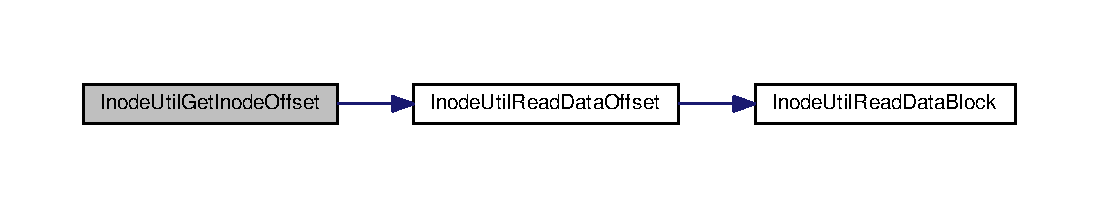
\includegraphics[width=350pt]{inodeproto_8h_a07685cf3d25b03c9e975af7d0f22ca81_cgraph}
\end{center}
\end{figure}


\hypertarget{inodeproto_8h_a63b7552b4e10719ea82758cb689850a8}{\index{inodeproto.\+h@{inodeproto.\+h}!Inode\+Util\+Is\+Free\+Inode@{Inode\+Util\+Is\+Free\+Inode}}
\index{Inode\+Util\+Is\+Free\+Inode@{Inode\+Util\+Is\+Free\+Inode}!inodeproto.\+h@{inodeproto.\+h}}
\subsubsection[{Inode\+Util\+Is\+Free\+Inode}]{\setlength{\rightskip}{0pt plus 5cm}I\+N\+T1 Inode\+Util\+Is\+Free\+Inode (
\begin{DoxyParamCaption}
\item[{struct ext3\+\_\+inode $\ast$}]{p\+Inode}
\end{DoxyParamCaption}
)}}\label{inodeproto_8h_a63b7552b4e10719ea82758cb689850a8}


 Function Name \+: Inode\+Util\+Is\+Free\+Inode

Author \+: Naveen Raj Selvaraj

Description \+: This Function is used to check if an inode is all zero

Input \+: p\+Inode -\/ pointer to the inode structure

Output \+: None

Returns \+: T\+R\+U\+E, if the inode is free F\+A\+L\+S\+E otherwise \hypertarget{inodeproto_8h_a6474c5fd62b8ca4f7745428690849175}{\index{inodeproto.\+h@{inodeproto.\+h}!Inode\+Util\+Print\+Children@{Inode\+Util\+Print\+Children}}
\index{Inode\+Util\+Print\+Children@{Inode\+Util\+Print\+Children}!inodeproto.\+h@{inodeproto.\+h}}
\subsubsection[{Inode\+Util\+Print\+Children}]{\setlength{\rightskip}{0pt plus 5cm}I\+N\+T4 Inode\+Util\+Print\+Children (
\begin{DoxyParamCaption}
\item[{U\+I\+N\+T4}]{u4\+Block\+No, }
\item[{U\+I\+N\+T4}]{u4\+Level}
\end{DoxyParamCaption}
)}}\label{inodeproto_8h_a6474c5fd62b8ca4f7745428690849175}


 Function Name \+: Inode\+Util\+Print\+Children

Author \+: Naveen Raj Selvaraj

Description \+: This Function is used to print the children of a directory inode as a part of printing the tree. If the child is a directory inode, then it calls the Inode\+Util\+Print\+Tree function to print the subtree of that child.

Input \+: u4\+Block\+No -\/ Data block of a directory inode u4\+Level -\/ number inidicating the depth of the file system object in the tree.(used to format the output)

Output \+: None

Returns \+: I\+N\+O\+D\+E\+\_\+\+S\+U\+C\+C\+E\+S\+S, when successfully printed I\+N\+O\+D\+E\+\_\+\+F\+A\+I\+L\+U\+R\+E otherwise 

Here is the call graph for this function\+:\nopagebreak
\begin{figure}[H]
\begin{center}
\leavevmode
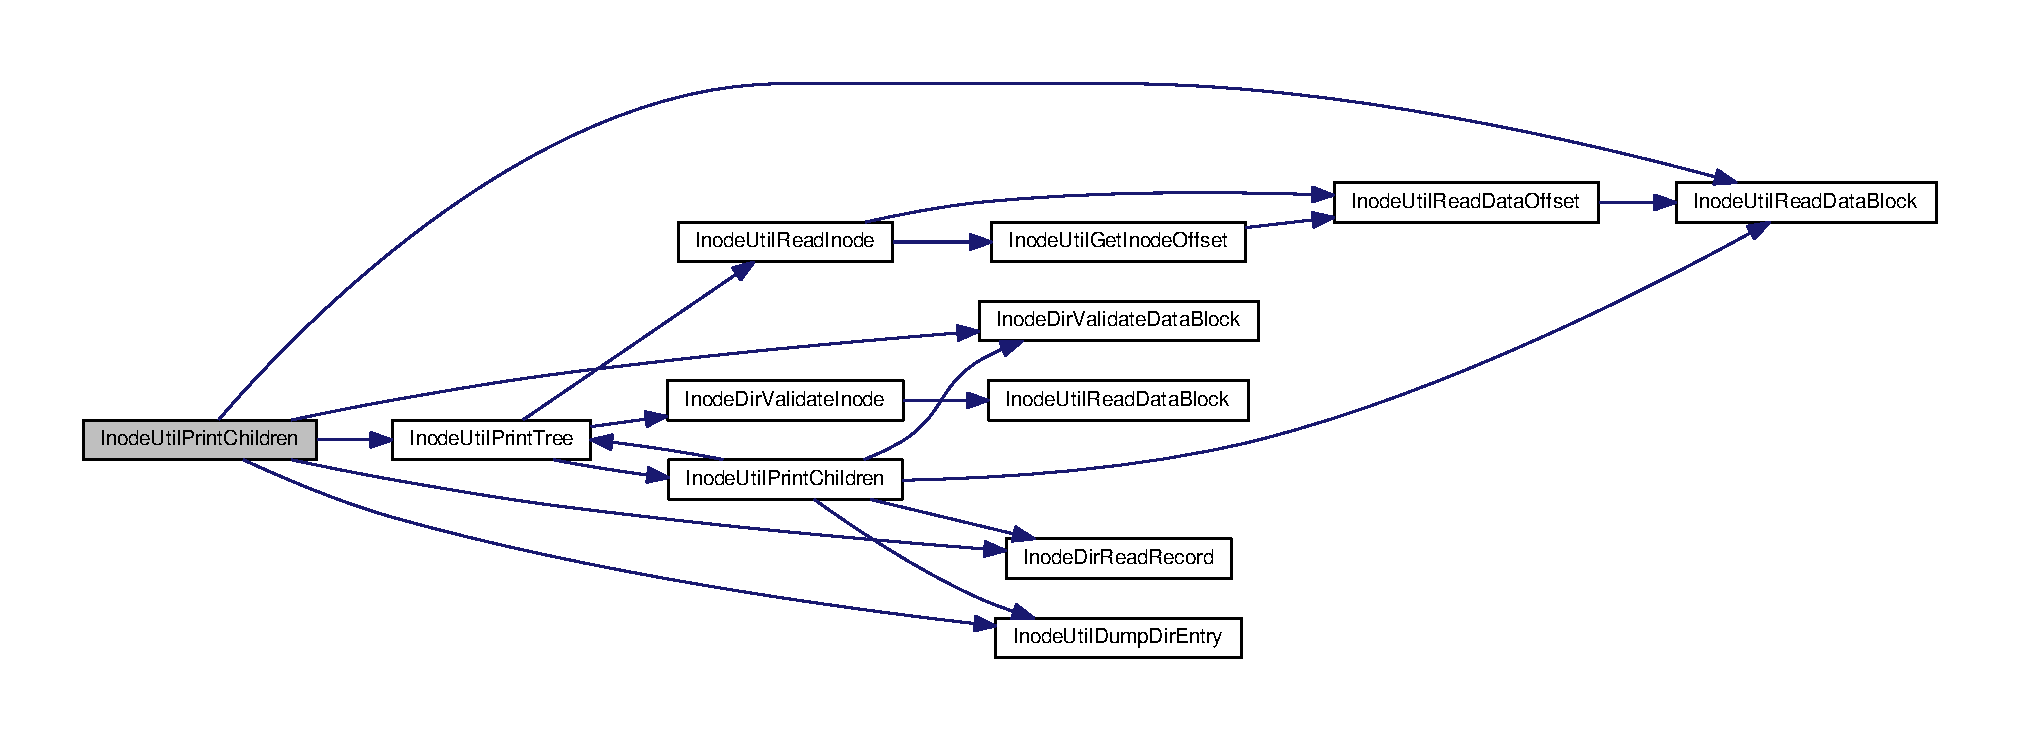
\includegraphics[width=350pt]{inodeproto_8h_a6474c5fd62b8ca4f7745428690849175_cgraph}
\end{center}
\end{figure}


\hypertarget{inodeproto_8h_a0bb419219a634fdfbb0e32df8fd4f937}{\index{inodeproto.\+h@{inodeproto.\+h}!Inode\+Util\+Print\+Dir\+Data\+Block@{Inode\+Util\+Print\+Dir\+Data\+Block}}
\index{Inode\+Util\+Print\+Dir\+Data\+Block@{Inode\+Util\+Print\+Dir\+Data\+Block}!inodeproto.\+h@{inodeproto.\+h}}
\subsubsection[{Inode\+Util\+Print\+Dir\+Data\+Block}]{\setlength{\rightskip}{0pt plus 5cm}I\+N\+T4 Inode\+Util\+Print\+Dir\+Data\+Block (
\begin{DoxyParamCaption}
\item[{U\+I\+N\+T4}]{u4\+Block\+No}
\end{DoxyParamCaption}
)}}\label{inodeproto_8h_a0bb419219a634fdfbb0e32df8fd4f937}


 Function Name \+: Inode\+Util\+Print\+Dir\+Data\+Block

Author \+: Naveen Raj Selvaraj

Description \+: This Function is used to print the directory entries present in a directory data block

Input \+: u4\+Block\+No -\/ directory data block number

Output \+: None

Returns \+: I\+N\+O\+D\+E\+\_\+\+S\+U\+C\+C\+E\+S\+S, when successfully printed I\+N\+O\+D\+E\+\_\+\+F\+A\+I\+L\+U\+R\+E otherwise 

Here is the call graph for this function\+:\nopagebreak
\begin{figure}[H]
\begin{center}
\leavevmode
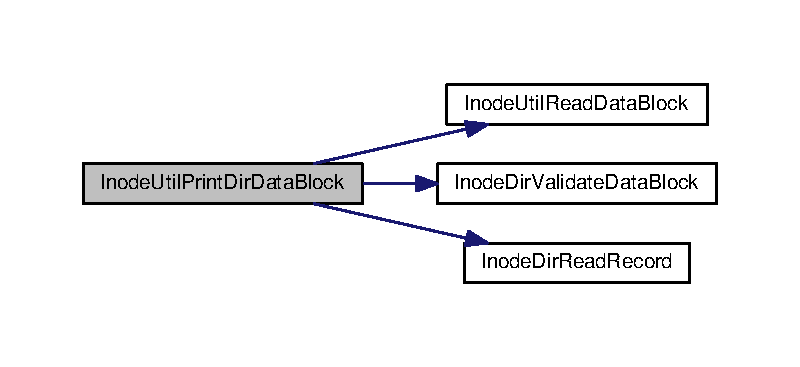
\includegraphics[width=350pt]{inodeproto_8h_a0bb419219a634fdfbb0e32df8fd4f937_cgraph}
\end{center}
\end{figure}


\hypertarget{inodeproto_8h_a45685e5c715aa741d487eae77c1083ae}{\index{inodeproto.\+h@{inodeproto.\+h}!Inode\+Util\+Print\+Inode@{Inode\+Util\+Print\+Inode}}
\index{Inode\+Util\+Print\+Inode@{Inode\+Util\+Print\+Inode}!inodeproto.\+h@{inodeproto.\+h}}
\subsubsection[{Inode\+Util\+Print\+Inode}]{\setlength{\rightskip}{0pt plus 5cm}I\+N\+T4 Inode\+Util\+Print\+Inode (
\begin{DoxyParamCaption}
\item[{U\+I\+N\+T4}]{u4\+Inode\+No}
\end{DoxyParamCaption}
)}}\label{inodeproto_8h_a45685e5c715aa741d487eae77c1083ae}


 Function Name \+: Inode\+Util\+Print\+Inode

Author \+: Naveen Raj Selvaraj

Description \+: This Function is used to print the contents of an inode

Input \+: u4\+Inode\+No -\/ Inode number

Output \+: None

Returns \+: I\+N\+O\+D\+E\+\_\+\+S\+U\+C\+C\+E\+S\+S, when successfully printed I\+N\+O\+D\+E\+\_\+\+F\+A\+I\+L\+U\+R\+E otherwise 

Here is the call graph for this function\+:\nopagebreak
\begin{figure}[H]
\begin{center}
\leavevmode
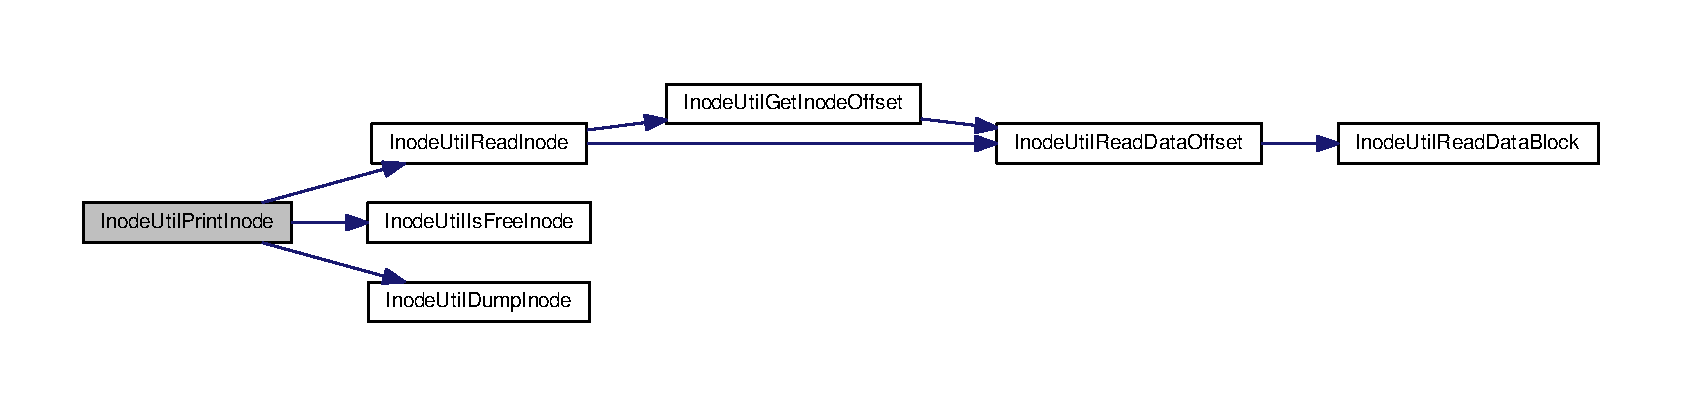
\includegraphics[width=350pt]{inodeproto_8h_a45685e5c715aa741d487eae77c1083ae_cgraph}
\end{center}
\end{figure}


\hypertarget{inodeproto_8h_af3bd13d59e79a9c574862e0a42ac1ac2}{\index{inodeproto.\+h@{inodeproto.\+h}!Inode\+Util\+Print\+Tree@{Inode\+Util\+Print\+Tree}}
\index{Inode\+Util\+Print\+Tree@{Inode\+Util\+Print\+Tree}!inodeproto.\+h@{inodeproto.\+h}}
\subsubsection[{Inode\+Util\+Print\+Tree}]{\setlength{\rightskip}{0pt plus 5cm}I\+N\+T4 Inode\+Util\+Print\+Tree (
\begin{DoxyParamCaption}
\item[{U\+I\+N\+T4}]{u4\+Inode\+No, }
\item[{U\+I\+N\+T4}]{u4\+Level}
\end{DoxyParamCaption}
)}}\label{inodeproto_8h_af3bd13d59e79a9c574862e0a42ac1ac2}


 Function Name \+: Inode\+Util\+Print\+Tree

Author \+: Naveen Raj Selvaraj

Description \+: This Function is used to print the tree/subtree of the file system objects starting at a specified directory inode in depth first order.

Input \+: u4\+Inode\+No -\/ Inode number u4\+Level -\/ number inidicating the depth of the file system object in the tree (this is used to format the output. e.\+g\+: root inode for the tree should be called with u4\+Level = 1) Output \+: None

Returns \+: I\+N\+O\+D\+E\+\_\+\+S\+U\+C\+C\+E\+S\+S, when successfully printed I\+N\+O\+D\+E\+\_\+\+F\+A\+I\+L\+U\+R\+E otherwise 

Here is the call graph for this function\+:\nopagebreak
\begin{figure}[H]
\begin{center}
\leavevmode
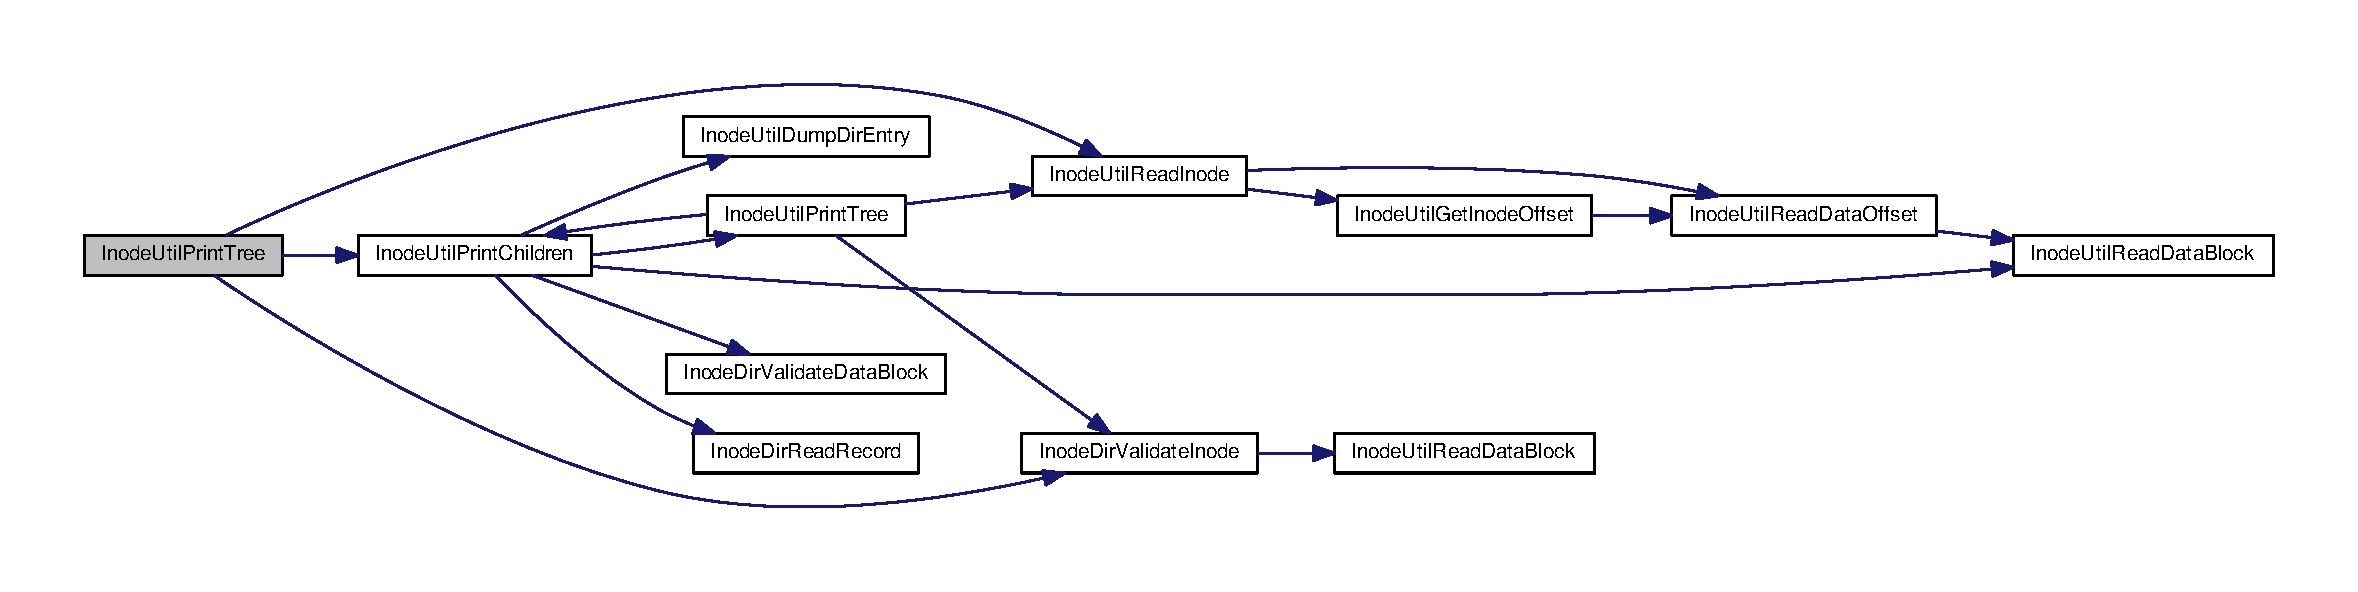
\includegraphics[width=350pt]{inodeproto_8h_af3bd13d59e79a9c574862e0a42ac1ac2_cgraph}
\end{center}
\end{figure}


\hypertarget{inodeproto_8h_a13b5c799edb137a494ad497145f59a56}{\index{inodeproto.\+h@{inodeproto.\+h}!Inode\+Util\+Read\+Data\+Block@{Inode\+Util\+Read\+Data\+Block}}
\index{Inode\+Util\+Read\+Data\+Block@{Inode\+Util\+Read\+Data\+Block}!inodeproto.\+h@{inodeproto.\+h}}
\subsubsection[{Inode\+Util\+Read\+Data\+Block}]{\setlength{\rightskip}{0pt plus 5cm}I\+N\+T4 Inode\+Util\+Read\+Data\+Block (
\begin{DoxyParamCaption}
\item[{U\+I\+N\+T4}]{u4\+Block\+No, }
\item[{U\+I\+N\+T2}]{u2\+Start\+Pos, }
\item[{V\+O\+I\+D $\ast$}]{p\+Buffer, }
\item[{U\+I\+N\+T4}]{u4\+Size}
\end{DoxyParamCaption}
)}}\label{inodeproto_8h_a13b5c799edb137a494ad497145f59a56}


 Function Name \+: Inode\+Util\+Read\+Data\+Block

Author \+: Naveen Raj Selvaraj

Description \+: This Function is used to read a file system block

Input \+: u4\+Block\+No -\/ Block number to read u4\+Size -\/ size of data to read in bytes

Output \+: p\+Buffer -\/ Buffer containg the contents of the block

Returns \+: I\+N\+O\+D\+E\+\_\+\+S\+U\+C\+C\+E\+S\+S, if the read succeeds I\+N\+O\+D\+E\+\_\+\+F\+A\+I\+L\+U\+R\+E otherwise \hypertarget{inodeproto_8h_a3add91b54cfb3e27f802ac8ab1b9ceb4}{\index{inodeproto.\+h@{inodeproto.\+h}!Inode\+Util\+Read\+Data\+Offset@{Inode\+Util\+Read\+Data\+Offset}}
\index{Inode\+Util\+Read\+Data\+Offset@{Inode\+Util\+Read\+Data\+Offset}!inodeproto.\+h@{inodeproto.\+h}}
\subsubsection[{Inode\+Util\+Read\+Data\+Offset}]{\setlength{\rightskip}{0pt plus 5cm}I\+N\+T4 Inode\+Util\+Read\+Data\+Offset (
\begin{DoxyParamCaption}
\item[{U\+I\+N\+T8}]{u8\+Offset, }
\item[{V\+O\+I\+D $\ast$}]{p\+Buffer, }
\item[{U\+I\+N\+T4}]{u4\+Size}
\end{DoxyParamCaption}
)}}\label{inodeproto_8h_a3add91b54cfb3e27f802ac8ab1b9ceb4}


 Function Name \+: Inode\+Util\+Read\+Data\+Offset

Author \+: Naveen Raj Selvaraj

Description \+: This Function is used to read data from any location

Input \+: u8\+Offset -\/ Byte offset to read u4\+Size -\/ size of data to read in bytes

Output \+: p\+Buffer -\/ Buffer containg the contents of the block

Returns \+: I\+N\+O\+D\+E\+\_\+\+S\+U\+C\+C\+E\+S\+S, if the read succeeds I\+N\+O\+D\+E\+\_\+\+F\+A\+I\+L\+U\+R\+E otherwise 

Here is the call graph for this function\+:\nopagebreak
\begin{figure}[H]
\begin{center}
\leavevmode
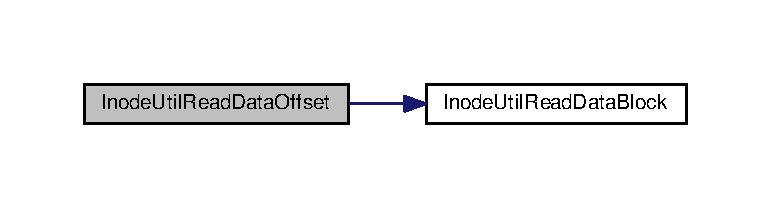
\includegraphics[width=350pt]{inodeproto_8h_a3add91b54cfb3e27f802ac8ab1b9ceb4_cgraph}
\end{center}
\end{figure}


\hypertarget{inodeproto_8h_a6867770228931c846eac7d67ffc582a0}{\index{inodeproto.\+h@{inodeproto.\+h}!Inode\+Util\+Read\+Inode@{Inode\+Util\+Read\+Inode}}
\index{Inode\+Util\+Read\+Inode@{Inode\+Util\+Read\+Inode}!inodeproto.\+h@{inodeproto.\+h}}
\subsubsection[{Inode\+Util\+Read\+Inode}]{\setlength{\rightskip}{0pt plus 5cm}I\+N\+T4 Inode\+Util\+Read\+Inode (
\begin{DoxyParamCaption}
\item[{U\+I\+N\+T4}]{u4\+Inode\+No, }
\item[{struct ext3\+\_\+inode $\ast$}]{p\+New\+Inode}
\end{DoxyParamCaption}
)}}\label{inodeproto_8h_a6867770228931c846eac7d67ffc582a0}


 Function Name \+: Inode\+Util\+Read\+Inode

Author \+: Naveen Raj Selvaraj

Description \+: This Function is used to read an inode

Input \+: u4\+Inode\+No -\/ Inode number to read

Output \+: p\+New\+Inode -\/ pointer to the structure containing the inode contents

Returns \+: I\+N\+O\+D\+E\+\_\+\+S\+U\+C\+C\+E\+S\+S, on successful read I\+N\+O\+D\+E\+\_\+\+F\+A\+I\+L\+U\+R\+E otherwise 

Here is the call graph for this function\+:\nopagebreak
\begin{figure}[H]
\begin{center}
\leavevmode
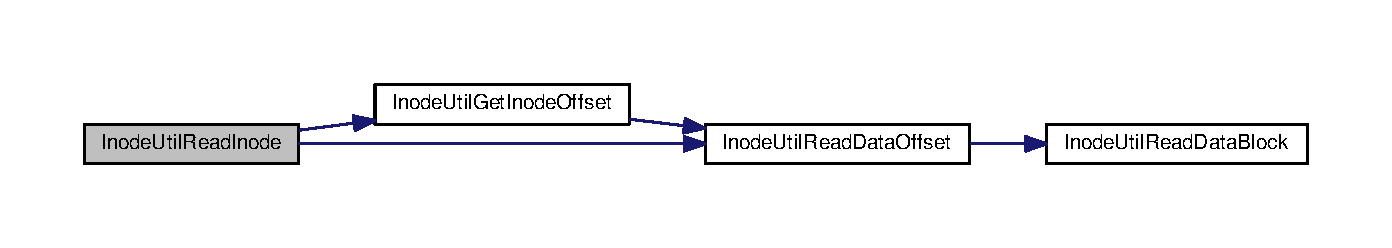
\includegraphics[width=350pt]{inodeproto_8h_a6867770228931c846eac7d67ffc582a0_cgraph}
\end{center}
\end{figure}


\hypertarget{inodeproto_8h_af4e29989b8cc9424603a4825af3491a0}{\index{inodeproto.\+h@{inodeproto.\+h}!Inode\+Util\+Write\+Data\+Block@{Inode\+Util\+Write\+Data\+Block}}
\index{Inode\+Util\+Write\+Data\+Block@{Inode\+Util\+Write\+Data\+Block}!inodeproto.\+h@{inodeproto.\+h}}
\subsubsection[{Inode\+Util\+Write\+Data\+Block}]{\setlength{\rightskip}{0pt plus 5cm}I\+N\+T4 Inode\+Util\+Write\+Data\+Block (
\begin{DoxyParamCaption}
\item[{U\+I\+N\+T4}]{u4\+Block\+No, }
\item[{U\+I\+N\+T2}]{u2\+Start\+Pos, }
\item[{V\+O\+I\+D $\ast$}]{p\+Buffer, }
\item[{U\+I\+N\+T4}]{u4\+Size}
\end{DoxyParamCaption}
)}}\label{inodeproto_8h_af4e29989b8cc9424603a4825af3491a0}


 Function Name \+: Inode\+Util\+Write\+Data\+Block

Author \+: Naveen Raj Selvaraj

Description \+: This Function is used to write data to a file system block

Input \+: u4\+Block\+No -\/ Block number to write u2\+Start\+Pos -\/ byte offset inside the block to start u4\+Size -\/ size of data to read in bytes p\+Buffer -\/ Buffer containg the data to write

Output \+: None

Returns \+: I\+N\+O\+D\+E\+\_\+\+S\+U\+C\+C\+E\+S\+S, if the write succeeds I\+N\+O\+D\+E\+\_\+\+F\+A\+I\+L\+U\+R\+E otherwise \hypertarget{inodeproto_8h_a9671fcb9023997872ade29c0241b0cab}{\index{inodeproto.\+h@{inodeproto.\+h}!Inode\+Util\+Write\+Data\+Offset@{Inode\+Util\+Write\+Data\+Offset}}
\index{Inode\+Util\+Write\+Data\+Offset@{Inode\+Util\+Write\+Data\+Offset}!inodeproto.\+h@{inodeproto.\+h}}
\subsubsection[{Inode\+Util\+Write\+Data\+Offset}]{\setlength{\rightskip}{0pt plus 5cm}I\+N\+T4 Inode\+Util\+Write\+Data\+Offset (
\begin{DoxyParamCaption}
\item[{U\+I\+N\+T8}]{u8\+Offset, }
\item[{V\+O\+I\+D $\ast$}]{p\+Buffer, }
\item[{U\+I\+N\+T4}]{u4\+Size}
\end{DoxyParamCaption}
)}}\label{inodeproto_8h_a9671fcb9023997872ade29c0241b0cab}


 Function Name \+: Inode\+Util\+Write\+Data\+Offset

Author \+: Naveen Raj Selvaraj

Description \+: This Function is used to write data at a particualar offset

Input \+: u8\+Offset -\/ Byte offset to write u4\+Size -\/ size of data to read in bytes p\+Buffer -\/ Buffer containg the data to write

Output \+: None

Returns \+: I\+N\+O\+D\+E\+\_\+\+S\+U\+C\+C\+E\+S\+S, if the write succeeds I\+N\+O\+D\+E\+\_\+\+F\+A\+I\+L\+U\+R\+E otherwise 

Here is the call graph for this function\+:\nopagebreak
\begin{figure}[H]
\begin{center}
\leavevmode
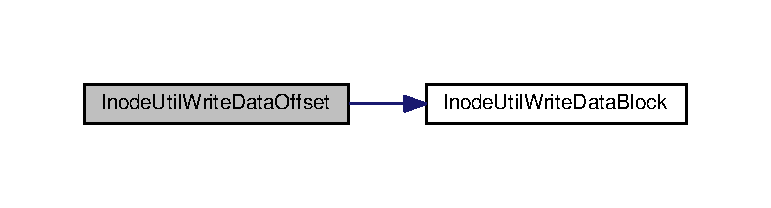
\includegraphics[width=350pt]{inodeproto_8h_a9671fcb9023997872ade29c0241b0cab_cgraph}
\end{center}
\end{figure}



\hypertarget{inodetdfs_8h}{\section{inc/inodetdfs.h File Reference}
\label{inodetdfs_8h}\index{inc/inodetdfs.\+h@{inc/inodetdfs.\+h}}
}
This graph shows which files directly or indirectly include this file\+:\nopagebreak
\begin{figure}[H]
\begin{center}
\leavevmode
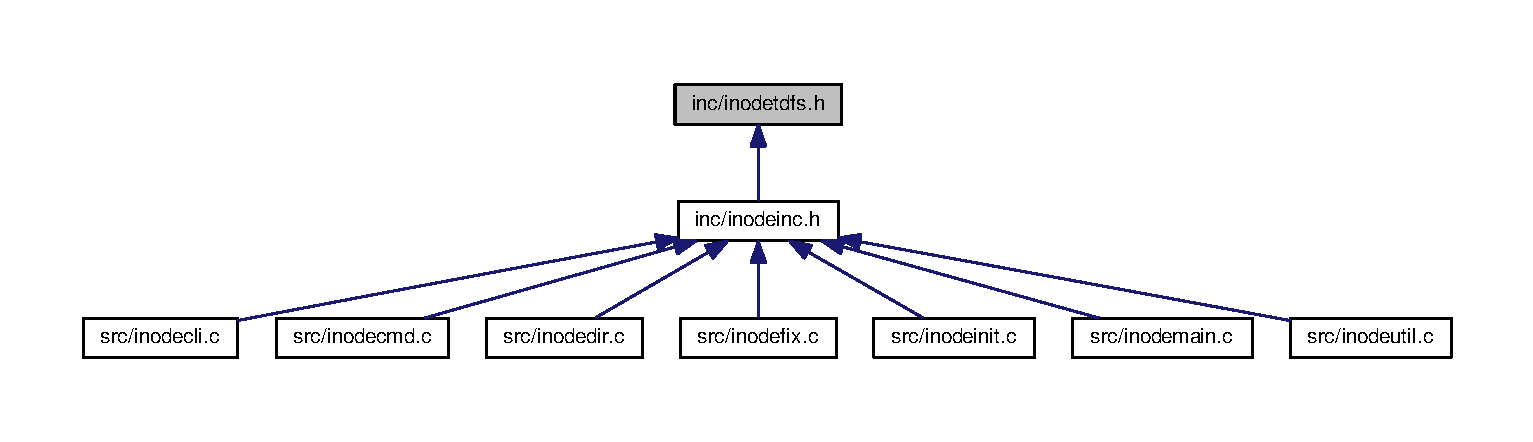
\includegraphics[width=350pt]{inodetdfs_8h__dep__incl}
\end{center}
\end{figure}
\subsection*{Typedefs}
\begin{DoxyCompactItemize}
\item 
typedef enum \hyperlink{inodetdfs_8h_a9c74355cbfc2148acfca8183926f9750}{file\+Filter\+\_\+e} \hyperlink{inodetdfs_8h_a408cefd7ee29ff67ed7fefab9393affa}{t\+File\+Filter}
\end{DoxyCompactItemize}
\subsection*{Enumerations}
\begin{DoxyCompactItemize}
\item 
enum \hyperlink{inodetdfs_8h_a9c74355cbfc2148acfca8183926f9750}{file\+Filter\+\_\+e} \{ \hyperlink{inodetdfs_8h_a9c74355cbfc2148acfca8183926f9750a758fd2fe70e1b30585d8080e1cc7ecd1}{F\+I\+L\+E\+\_\+\+T\+Y\+P\+E\+\_\+\+D\+I\+R\+S}, 
\hyperlink{inodetdfs_8h_a9c74355cbfc2148acfca8183926f9750aad6bf67080dda41a0f05c25621a1b05e}{F\+I\+L\+E\+\_\+\+T\+Y\+P\+E\+\_\+\+F\+I\+L\+E\+S}, 
\hyperlink{inodetdfs_8h_a9c74355cbfc2148acfca8183926f9750a12e83d3f705d2ca79fcacc62ca4e9e1f}{F\+I\+L\+E\+\_\+\+T\+Y\+P\+E\+\_\+\+A\+L\+L}
 \}
\item 
enum \{ \hyperlink{inodetdfs_8h_a99fb83031ce9923c84392b4e92f956b5a5a782ca7a5216fdcfb9ff6fb4666525f}{F\+I\+L\+E\+\_\+\+T\+Y\+P\+E\+\_\+\+U\+N\+K\+N\+O\+W\+N} = 0, 
\hyperlink{inodetdfs_8h_a99fb83031ce9923c84392b4e92f956b5a0fa88135dba520076ded539764367d2c}{F\+I\+L\+E\+\_\+\+T\+Y\+P\+E\+\_\+\+F\+I\+L\+E} = 1, 
\hyperlink{inodetdfs_8h_a99fb83031ce9923c84392b4e92f956b5aebcae9d844ae4c0785cb14f17c8481ec}{F\+I\+L\+E\+\_\+\+T\+Y\+P\+E\+\_\+\+D\+I\+R} = 2
 \}
\item 
enum \{ \hyperlink{inodetdfs_8h_abc6126af1d45847bc59afa0aa3216b04a7297644c9cdf6520723ffd6aa029ae97}{I\+N\+O\+D\+E\+\_\+\+C\+O\+R\+R\+U\+P\+T} =1, 
\hyperlink{inodetdfs_8h_abc6126af1d45847bc59afa0aa3216b04a072d2cd58191d51f0faebaeb9db3bf7e}{I\+N\+O\+D\+E\+\_\+\+F\+I\+X} =2
 \}
\end{DoxyCompactItemize}


\subsection{Typedef Documentation}
\hypertarget{inodetdfs_8h_a408cefd7ee29ff67ed7fefab9393affa}{\index{inodetdfs.\+h@{inodetdfs.\+h}!t\+File\+Filter@{t\+File\+Filter}}
\index{t\+File\+Filter@{t\+File\+Filter}!inodetdfs.\+h@{inodetdfs.\+h}}
\subsubsection[{t\+File\+Filter}]{\setlength{\rightskip}{0pt plus 5cm}typedef enum {\bf file\+Filter\+\_\+e} {\bf t\+File\+Filter}}}\label{inodetdfs_8h_a408cefd7ee29ff67ed7fefab9393affa}


\subsection{Enumeration Type Documentation}
\hypertarget{inodetdfs_8h_a99fb83031ce9923c84392b4e92f956b5}{\subsubsection[{anonymous enum}]{\setlength{\rightskip}{0pt plus 5cm}anonymous enum}}\label{inodetdfs_8h_a99fb83031ce9923c84392b4e92f956b5}
\begin{Desc}
\item[Enumerator]\par
\begin{description}
\index{F\+I\+L\+E\+\_\+\+T\+Y\+P\+E\+\_\+\+U\+N\+K\+N\+O\+W\+N@{F\+I\+L\+E\+\_\+\+T\+Y\+P\+E\+\_\+\+U\+N\+K\+N\+O\+W\+N}!inodetdfs.\+h@{inodetdfs.\+h}}\index{inodetdfs.\+h@{inodetdfs.\+h}!F\+I\+L\+E\+\_\+\+T\+Y\+P\+E\+\_\+\+U\+N\+K\+N\+O\+W\+N@{F\+I\+L\+E\+\_\+\+T\+Y\+P\+E\+\_\+\+U\+N\+K\+N\+O\+W\+N}}\item[{\em 
\hypertarget{inodetdfs_8h_a99fb83031ce9923c84392b4e92f956b5a5a782ca7a5216fdcfb9ff6fb4666525f}{F\+I\+L\+E\+\_\+\+T\+Y\+P\+E\+\_\+\+U\+N\+K\+N\+O\+W\+N}\label{inodetdfs_8h_a99fb83031ce9923c84392b4e92f956b5a5a782ca7a5216fdcfb9ff6fb4666525f}
}]\index{F\+I\+L\+E\+\_\+\+T\+Y\+P\+E\+\_\+\+F\+I\+L\+E@{F\+I\+L\+E\+\_\+\+T\+Y\+P\+E\+\_\+\+F\+I\+L\+E}!inodetdfs.\+h@{inodetdfs.\+h}}\index{inodetdfs.\+h@{inodetdfs.\+h}!F\+I\+L\+E\+\_\+\+T\+Y\+P\+E\+\_\+\+F\+I\+L\+E@{F\+I\+L\+E\+\_\+\+T\+Y\+P\+E\+\_\+\+F\+I\+L\+E}}\item[{\em 
\hypertarget{inodetdfs_8h_a99fb83031ce9923c84392b4e92f956b5a0fa88135dba520076ded539764367d2c}{F\+I\+L\+E\+\_\+\+T\+Y\+P\+E\+\_\+\+F\+I\+L\+E}\label{inodetdfs_8h_a99fb83031ce9923c84392b4e92f956b5a0fa88135dba520076ded539764367d2c}
}]\index{F\+I\+L\+E\+\_\+\+T\+Y\+P\+E\+\_\+\+D\+I\+R@{F\+I\+L\+E\+\_\+\+T\+Y\+P\+E\+\_\+\+D\+I\+R}!inodetdfs.\+h@{inodetdfs.\+h}}\index{inodetdfs.\+h@{inodetdfs.\+h}!F\+I\+L\+E\+\_\+\+T\+Y\+P\+E\+\_\+\+D\+I\+R@{F\+I\+L\+E\+\_\+\+T\+Y\+P\+E\+\_\+\+D\+I\+R}}\item[{\em 
\hypertarget{inodetdfs_8h_a99fb83031ce9923c84392b4e92f956b5aebcae9d844ae4c0785cb14f17c8481ec}{F\+I\+L\+E\+\_\+\+T\+Y\+P\+E\+\_\+\+D\+I\+R}\label{inodetdfs_8h_a99fb83031ce9923c84392b4e92f956b5aebcae9d844ae4c0785cb14f17c8481ec}
}]\end{description}
\end{Desc}
\hypertarget{inodetdfs_8h_abc6126af1d45847bc59afa0aa3216b04}{\subsubsection[{anonymous enum}]{\setlength{\rightskip}{0pt plus 5cm}anonymous enum}}\label{inodetdfs_8h_abc6126af1d45847bc59afa0aa3216b04}
\begin{Desc}
\item[Enumerator]\par
\begin{description}
\index{I\+N\+O\+D\+E\+\_\+\+C\+O\+R\+R\+U\+P\+T@{I\+N\+O\+D\+E\+\_\+\+C\+O\+R\+R\+U\+P\+T}!inodetdfs.\+h@{inodetdfs.\+h}}\index{inodetdfs.\+h@{inodetdfs.\+h}!I\+N\+O\+D\+E\+\_\+\+C\+O\+R\+R\+U\+P\+T@{I\+N\+O\+D\+E\+\_\+\+C\+O\+R\+R\+U\+P\+T}}\item[{\em 
\hypertarget{inodetdfs_8h_abc6126af1d45847bc59afa0aa3216b04a7297644c9cdf6520723ffd6aa029ae97}{I\+N\+O\+D\+E\+\_\+\+C\+O\+R\+R\+U\+P\+T}\label{inodetdfs_8h_abc6126af1d45847bc59afa0aa3216b04a7297644c9cdf6520723ffd6aa029ae97}
}]\index{I\+N\+O\+D\+E\+\_\+\+F\+I\+X@{I\+N\+O\+D\+E\+\_\+\+F\+I\+X}!inodetdfs.\+h@{inodetdfs.\+h}}\index{inodetdfs.\+h@{inodetdfs.\+h}!I\+N\+O\+D\+E\+\_\+\+F\+I\+X@{I\+N\+O\+D\+E\+\_\+\+F\+I\+X}}\item[{\em 
\hypertarget{inodetdfs_8h_abc6126af1d45847bc59afa0aa3216b04a072d2cd58191d51f0faebaeb9db3bf7e}{I\+N\+O\+D\+E\+\_\+\+F\+I\+X}\label{inodetdfs_8h_abc6126af1d45847bc59afa0aa3216b04a072d2cd58191d51f0faebaeb9db3bf7e}
}]\end{description}
\end{Desc}
\hypertarget{inodetdfs_8h_a9c74355cbfc2148acfca8183926f9750}{\index{inodetdfs.\+h@{inodetdfs.\+h}!file\+Filter\+\_\+e@{file\+Filter\+\_\+e}}
\index{file\+Filter\+\_\+e@{file\+Filter\+\_\+e}!inodetdfs.\+h@{inodetdfs.\+h}}
\subsubsection[{file\+Filter\+\_\+e}]{\setlength{\rightskip}{0pt plus 5cm}enum {\bf file\+Filter\+\_\+e}}}\label{inodetdfs_8h_a9c74355cbfc2148acfca8183926f9750}
\begin{Desc}
\item[Enumerator]\par
\begin{description}
\index{F\+I\+L\+E\+\_\+\+T\+Y\+P\+E\+\_\+\+D\+I\+R\+S@{F\+I\+L\+E\+\_\+\+T\+Y\+P\+E\+\_\+\+D\+I\+R\+S}!inodetdfs.\+h@{inodetdfs.\+h}}\index{inodetdfs.\+h@{inodetdfs.\+h}!F\+I\+L\+E\+\_\+\+T\+Y\+P\+E\+\_\+\+D\+I\+R\+S@{F\+I\+L\+E\+\_\+\+T\+Y\+P\+E\+\_\+\+D\+I\+R\+S}}\item[{\em 
\hypertarget{inodetdfs_8h_a9c74355cbfc2148acfca8183926f9750a758fd2fe70e1b30585d8080e1cc7ecd1}{F\+I\+L\+E\+\_\+\+T\+Y\+P\+E\+\_\+\+D\+I\+R\+S}\label{inodetdfs_8h_a9c74355cbfc2148acfca8183926f9750a758fd2fe70e1b30585d8080e1cc7ecd1}
}]\index{F\+I\+L\+E\+\_\+\+T\+Y\+P\+E\+\_\+\+F\+I\+L\+E\+S@{F\+I\+L\+E\+\_\+\+T\+Y\+P\+E\+\_\+\+F\+I\+L\+E\+S}!inodetdfs.\+h@{inodetdfs.\+h}}\index{inodetdfs.\+h@{inodetdfs.\+h}!F\+I\+L\+E\+\_\+\+T\+Y\+P\+E\+\_\+\+F\+I\+L\+E\+S@{F\+I\+L\+E\+\_\+\+T\+Y\+P\+E\+\_\+\+F\+I\+L\+E\+S}}\item[{\em 
\hypertarget{inodetdfs_8h_a9c74355cbfc2148acfca8183926f9750aad6bf67080dda41a0f05c25621a1b05e}{F\+I\+L\+E\+\_\+\+T\+Y\+P\+E\+\_\+\+F\+I\+L\+E\+S}\label{inodetdfs_8h_a9c74355cbfc2148acfca8183926f9750aad6bf67080dda41a0f05c25621a1b05e}
}]\index{F\+I\+L\+E\+\_\+\+T\+Y\+P\+E\+\_\+\+A\+L\+L@{F\+I\+L\+E\+\_\+\+T\+Y\+P\+E\+\_\+\+A\+L\+L}!inodetdfs.\+h@{inodetdfs.\+h}}\index{inodetdfs.\+h@{inodetdfs.\+h}!F\+I\+L\+E\+\_\+\+T\+Y\+P\+E\+\_\+\+A\+L\+L@{F\+I\+L\+E\+\_\+\+T\+Y\+P\+E\+\_\+\+A\+L\+L}}\item[{\em 
\hypertarget{inodetdfs_8h_a9c74355cbfc2148acfca8183926f9750a12e83d3f705d2ca79fcacc62ca4e9e1f}{F\+I\+L\+E\+\_\+\+T\+Y\+P\+E\+\_\+\+A\+L\+L}\label{inodetdfs_8h_a9c74355cbfc2148acfca8183926f9750a12e83d3f705d2ca79fcacc62ca4e9e1f}
}]\end{description}
\end{Desc}

\hypertarget{inodetime_8h}{\section{inc/inodetime.h File Reference}
\label{inodetime_8h}\index{inc/inodetime.\+h@{inc/inodetime.\+h}}
}
This graph shows which files directly or indirectly include this file\+:\nopagebreak
\begin{figure}[H]
\begin{center}
\leavevmode
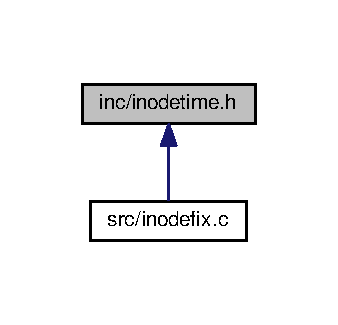
\includegraphics[width=162pt]{inodetime_8h__dep__incl}
\end{center}
\end{figure}
\subsection*{Variables}
\begin{DoxyCompactItemize}
\item 
struct timeval \hyperlink{inodetime_8h_a36edfd0296c32a795b36ea4fa7154cc5}{g\+End\+Time}
\item 
struct timeval \hyperlink{inodetime_8h_a6d91f0b5c171137ba9a5213f6c6f98f8}{g\+Start\+Time}
\end{DoxyCompactItemize}


\subsection{Variable Documentation}
\hypertarget{inodetime_8h_a36edfd0296c32a795b36ea4fa7154cc5}{\index{inodetime.\+h@{inodetime.\+h}!g\+End\+Time@{g\+End\+Time}}
\index{g\+End\+Time@{g\+End\+Time}!inodetime.\+h@{inodetime.\+h}}
\subsubsection[{g\+End\+Time}]{\setlength{\rightskip}{0pt plus 5cm}struct timeval g\+End\+Time}}\label{inodetime_8h_a36edfd0296c32a795b36ea4fa7154cc5}
\hypertarget{inodetime_8h_a6d91f0b5c171137ba9a5213f6c6f98f8}{\index{inodetime.\+h@{inodetime.\+h}!g\+Start\+Time@{g\+Start\+Time}}
\index{g\+Start\+Time@{g\+Start\+Time}!inodetime.\+h@{inodetime.\+h}}
\subsubsection[{g\+Start\+Time}]{\setlength{\rightskip}{0pt plus 5cm}struct timeval g\+Start\+Time}}\label{inodetime_8h_a6d91f0b5c171137ba9a5213f6c6f98f8}

\hypertarget{make_8h}{\section{make.\+h File Reference}
\label{make_8h}\index{make.\+h@{make.\+h}}
}

\hypertarget{inodecli_8c}{\section{src/inodecli.c File Reference}
\label{inodecli_8c}\index{src/inodecli.\+c@{src/inodecli.\+c}}
}
{\ttfamily \#include \char`\"{}inodeinc.\+h\char`\"{}}\\*
{\ttfamily \#include \char`\"{}inodecli.\+h\char`\"{}}\\*
Include dependency graph for inodecli.\+c\+:\nopagebreak
\begin{figure}[H]
\begin{center}
\leavevmode
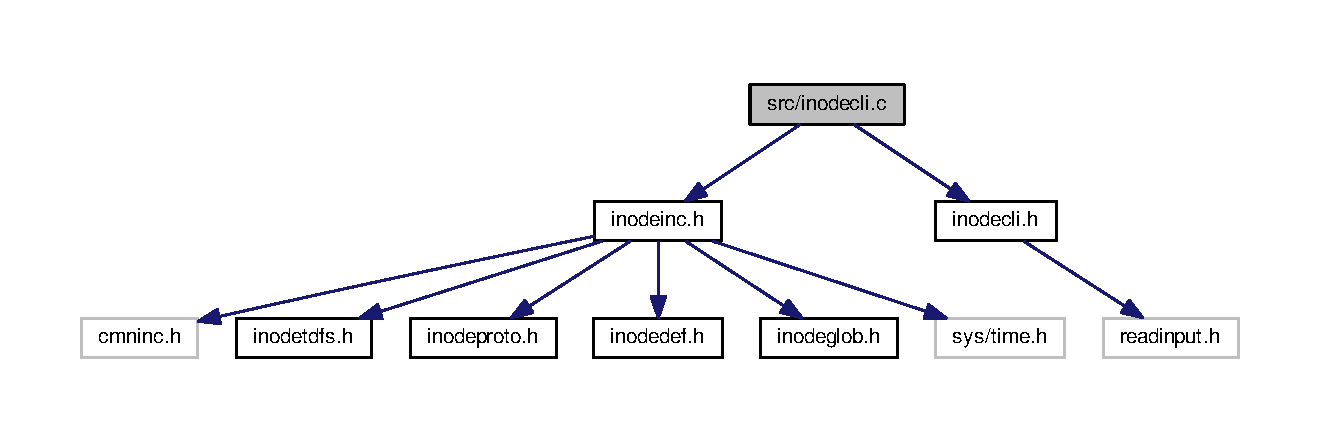
\includegraphics[width=350pt]{inodecli_8c__incl}
\end{center}
\end{figure}
\subsection*{Functions}
\begin{DoxyCompactItemize}
\item 
V\+O\+I\+D \hyperlink{inodecli_8c_aa0b53520e1018955fde7aea285159808}{Inode\+Cli\+Start} ()
\item 
V\+O\+I\+D \hyperlink{inodecli_8c_adde588bd205c9ef530fa02ef8f48cf69}{Inode\+Cli\+Handle\+Cmd} (C\+H\+A\+R $\ast$p\+Cmd)
\item 
V\+O\+I\+D \hyperlink{inodecli_8c_a3157714cddf8864e002915be47a6cef5}{Inode\+Cli\+Cmd\+Action} (\hyperlink{inodecli_8h_a5a66cd47ebf8f625f42d8df880975e95}{t\+Command} cmd)
\item 
I\+N\+T1 \hyperlink{inodecli_8c_adaf1a711f6592434c4f1280c0a92fd22}{Inode\+Cli\+Parse\+Cmd} (C\+H\+A\+R $\ast$p\+Cmd\+Str, \hyperlink{inodecli_8h_a5a66cd47ebf8f625f42d8df880975e95}{t\+Command} $\ast$p\+Cmd)
\item 
I\+N\+T1 \hyperlink{inodecli_8c_af594f3b863f653a969da942bc1cafe7c}{Inode\+Cli\+Validate\+Cmd} (\hyperlink{inodecli_8h_a5a66cd47ebf8f625f42d8df880975e95}{t\+Command} $\ast$p\+Cmd, U\+I\+N\+T1 u1\+Arg\+C)
\end{DoxyCompactItemize}
\subsection*{Variables}
\begin{DoxyCompactItemize}
\item 
\hyperlink{inodecli_8h_a25509e56046d94d7ebcb24fb035f12c1}{t\+Cmd} \hyperlink{inodecli_8c_a72a268537701a29a14740ed4d190f1f0}{g\+Commands} \mbox{[}\hyperlink{inodecli_8h_a06fc87d81c62e9abb8790b6e5713c55ba0b2e221172240c1b6e6cea012317fb16}{C\+M\+D\+\_\+\+I\+D\+\_\+\+M\+A\+X}\mbox{]}
\item 
U\+I\+N\+T1 \hyperlink{inodecli_8c_ac732f1e6c26e35b8e7fbb38498b415e4}{gu1\+Exit}
\end{DoxyCompactItemize}


\subsection{Function Documentation}
\hypertarget{inodecli_8c_a3157714cddf8864e002915be47a6cef5}{\index{inodecli.\+c@{inodecli.\+c}!Inode\+Cli\+Cmd\+Action@{Inode\+Cli\+Cmd\+Action}}
\index{Inode\+Cli\+Cmd\+Action@{Inode\+Cli\+Cmd\+Action}!inodecli.\+c@{inodecli.\+c}}
\subsubsection[{Inode\+Cli\+Cmd\+Action}]{\setlength{\rightskip}{0pt plus 5cm}V\+O\+I\+D Inode\+Cli\+Cmd\+Action (
\begin{DoxyParamCaption}
\item[{{\bf t\+Command}}]{cmd}
\end{DoxyParamCaption}
)}}\label{inodecli_8c_a3157714cddf8864e002915be47a6cef5}


 Function Name \+: Inode\+Cli\+Cmd\+Action

Description \+: This Function is the overall action handler. This function identifies the command and the action to be taken for the command.

Input \+: cmd -\/ structure containing the parsed command and arguments

Output \+: None

Returns \+: None 

Here is the call graph for this function\+:\nopagebreak
\begin{figure}[H]
\begin{center}
\leavevmode
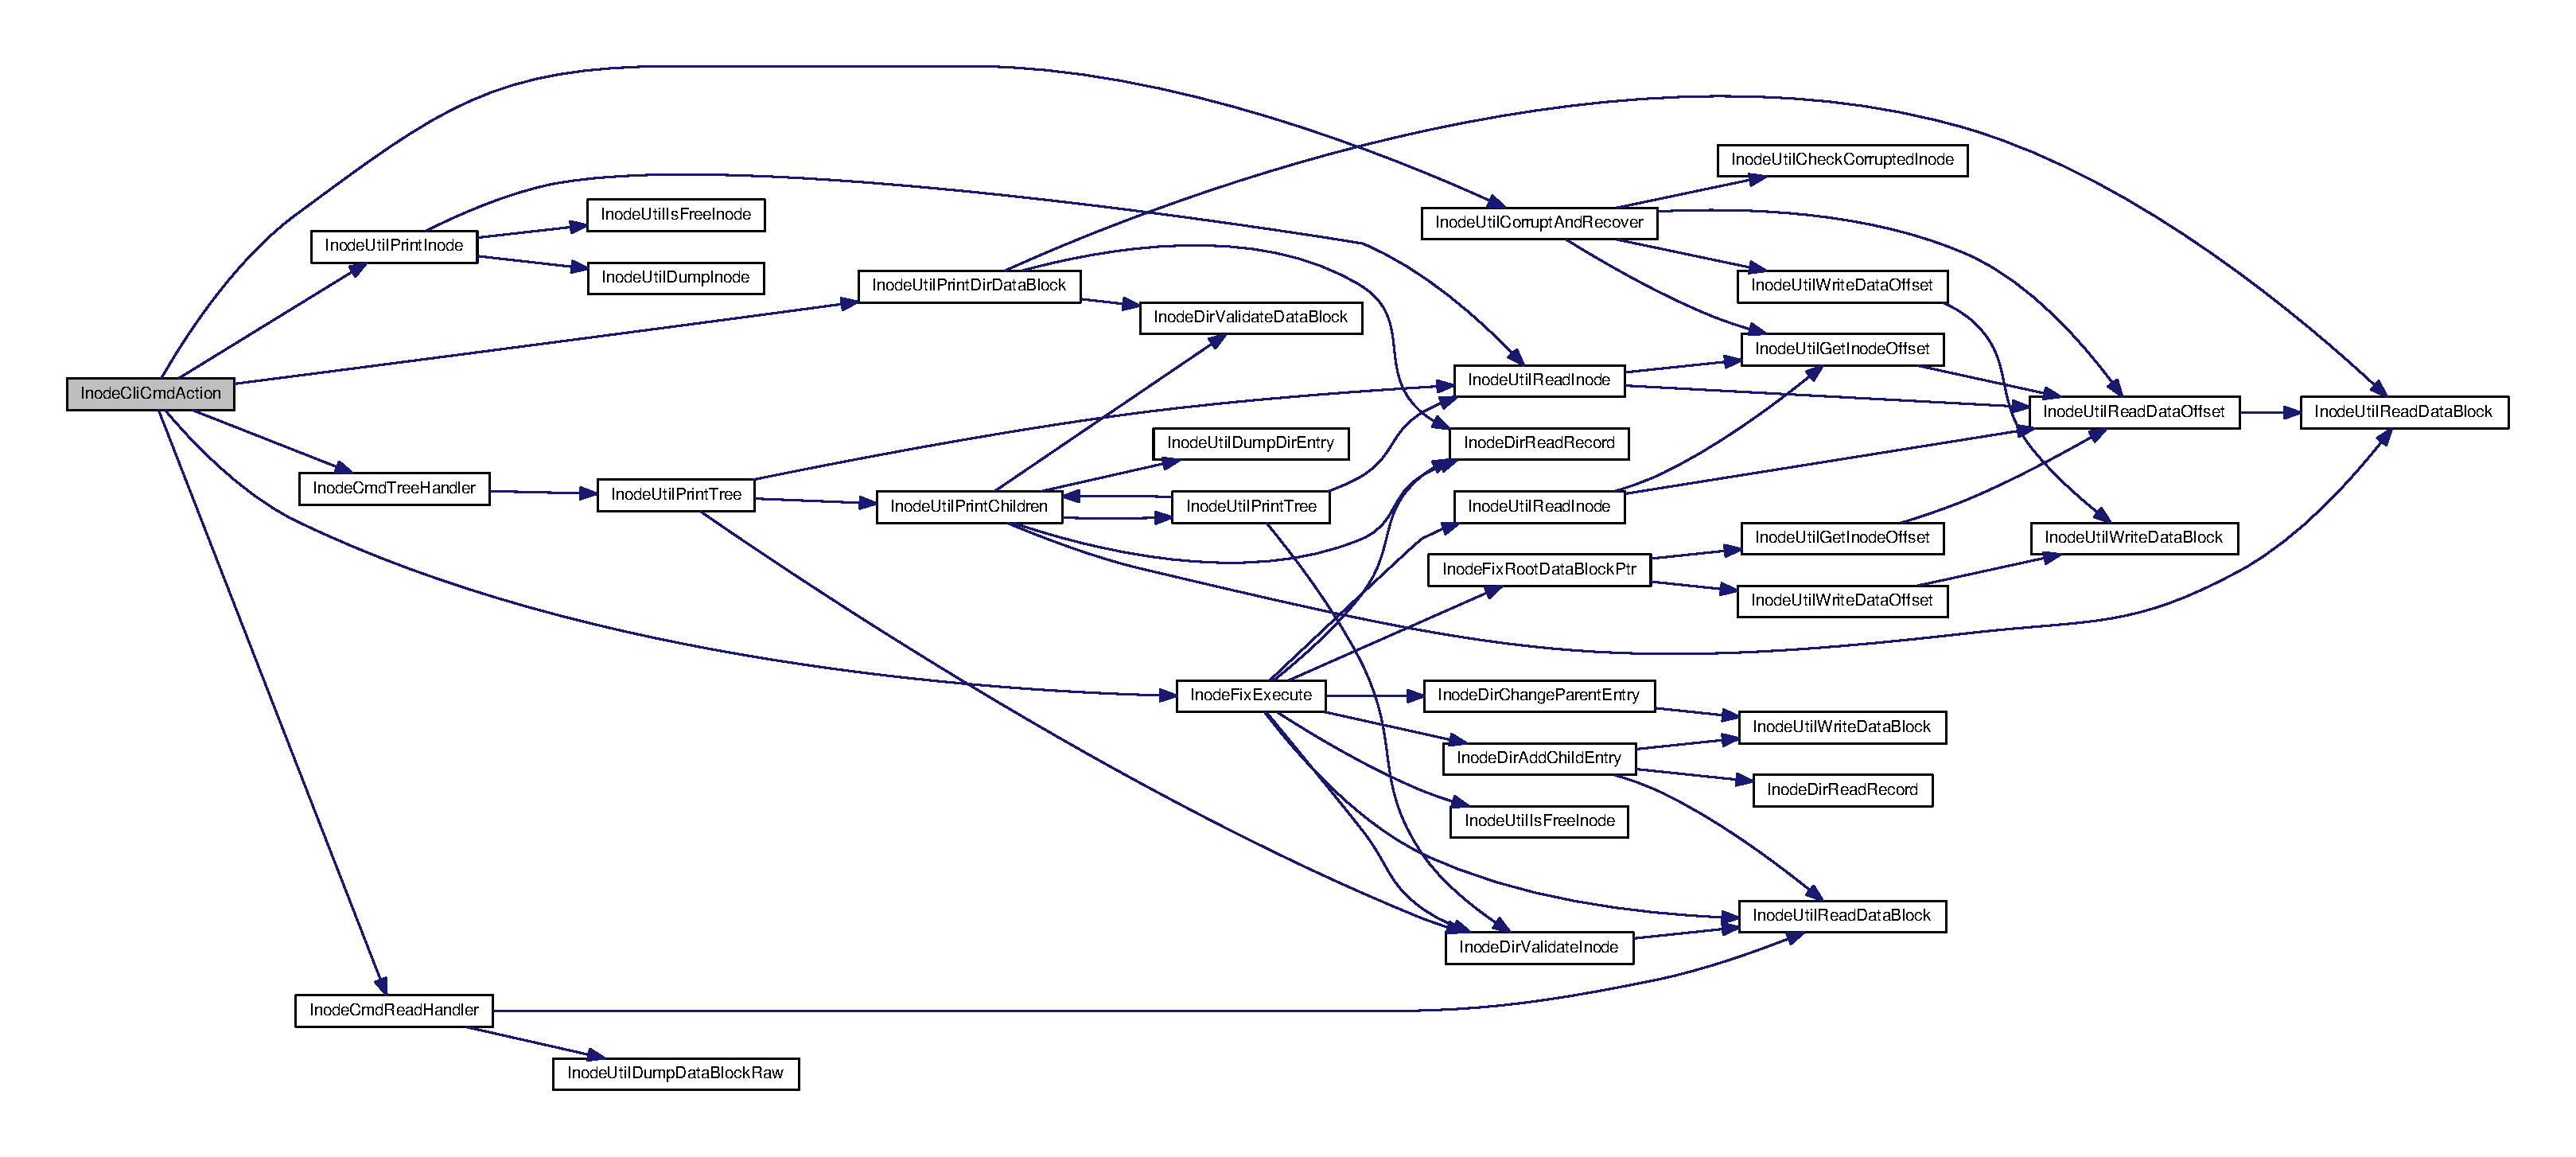
\includegraphics[width=350pt]{inodecli_8c_a3157714cddf8864e002915be47a6cef5_cgraph}
\end{center}
\end{figure}


\hypertarget{inodecli_8c_adde588bd205c9ef530fa02ef8f48cf69}{\index{inodecli.\+c@{inodecli.\+c}!Inode\+Cli\+Handle\+Cmd@{Inode\+Cli\+Handle\+Cmd}}
\index{Inode\+Cli\+Handle\+Cmd@{Inode\+Cli\+Handle\+Cmd}!inodecli.\+c@{inodecli.\+c}}
\subsubsection[{Inode\+Cli\+Handle\+Cmd}]{\setlength{\rightskip}{0pt plus 5cm}V\+O\+I\+D Inode\+Cli\+Handle\+Cmd (
\begin{DoxyParamCaption}
\item[{C\+H\+A\+R $\ast$}]{p\+Cmd}
\end{DoxyParamCaption}
)}}\label{inodecli_8c_adde588bd205c9ef530fa02ef8f48cf69}


 Function Name \+: Inode\+Cli\+Handle

Description \+: This Function tries to parse the command input and if it succeeds then calls the high level action handler function with the parsed command.

Input \+: p\+Cmd -\/ Command string input from the user

Output \+: None

Returns \+: None 

Here is the call graph for this function\+:\nopagebreak
\begin{figure}[H]
\begin{center}
\leavevmode
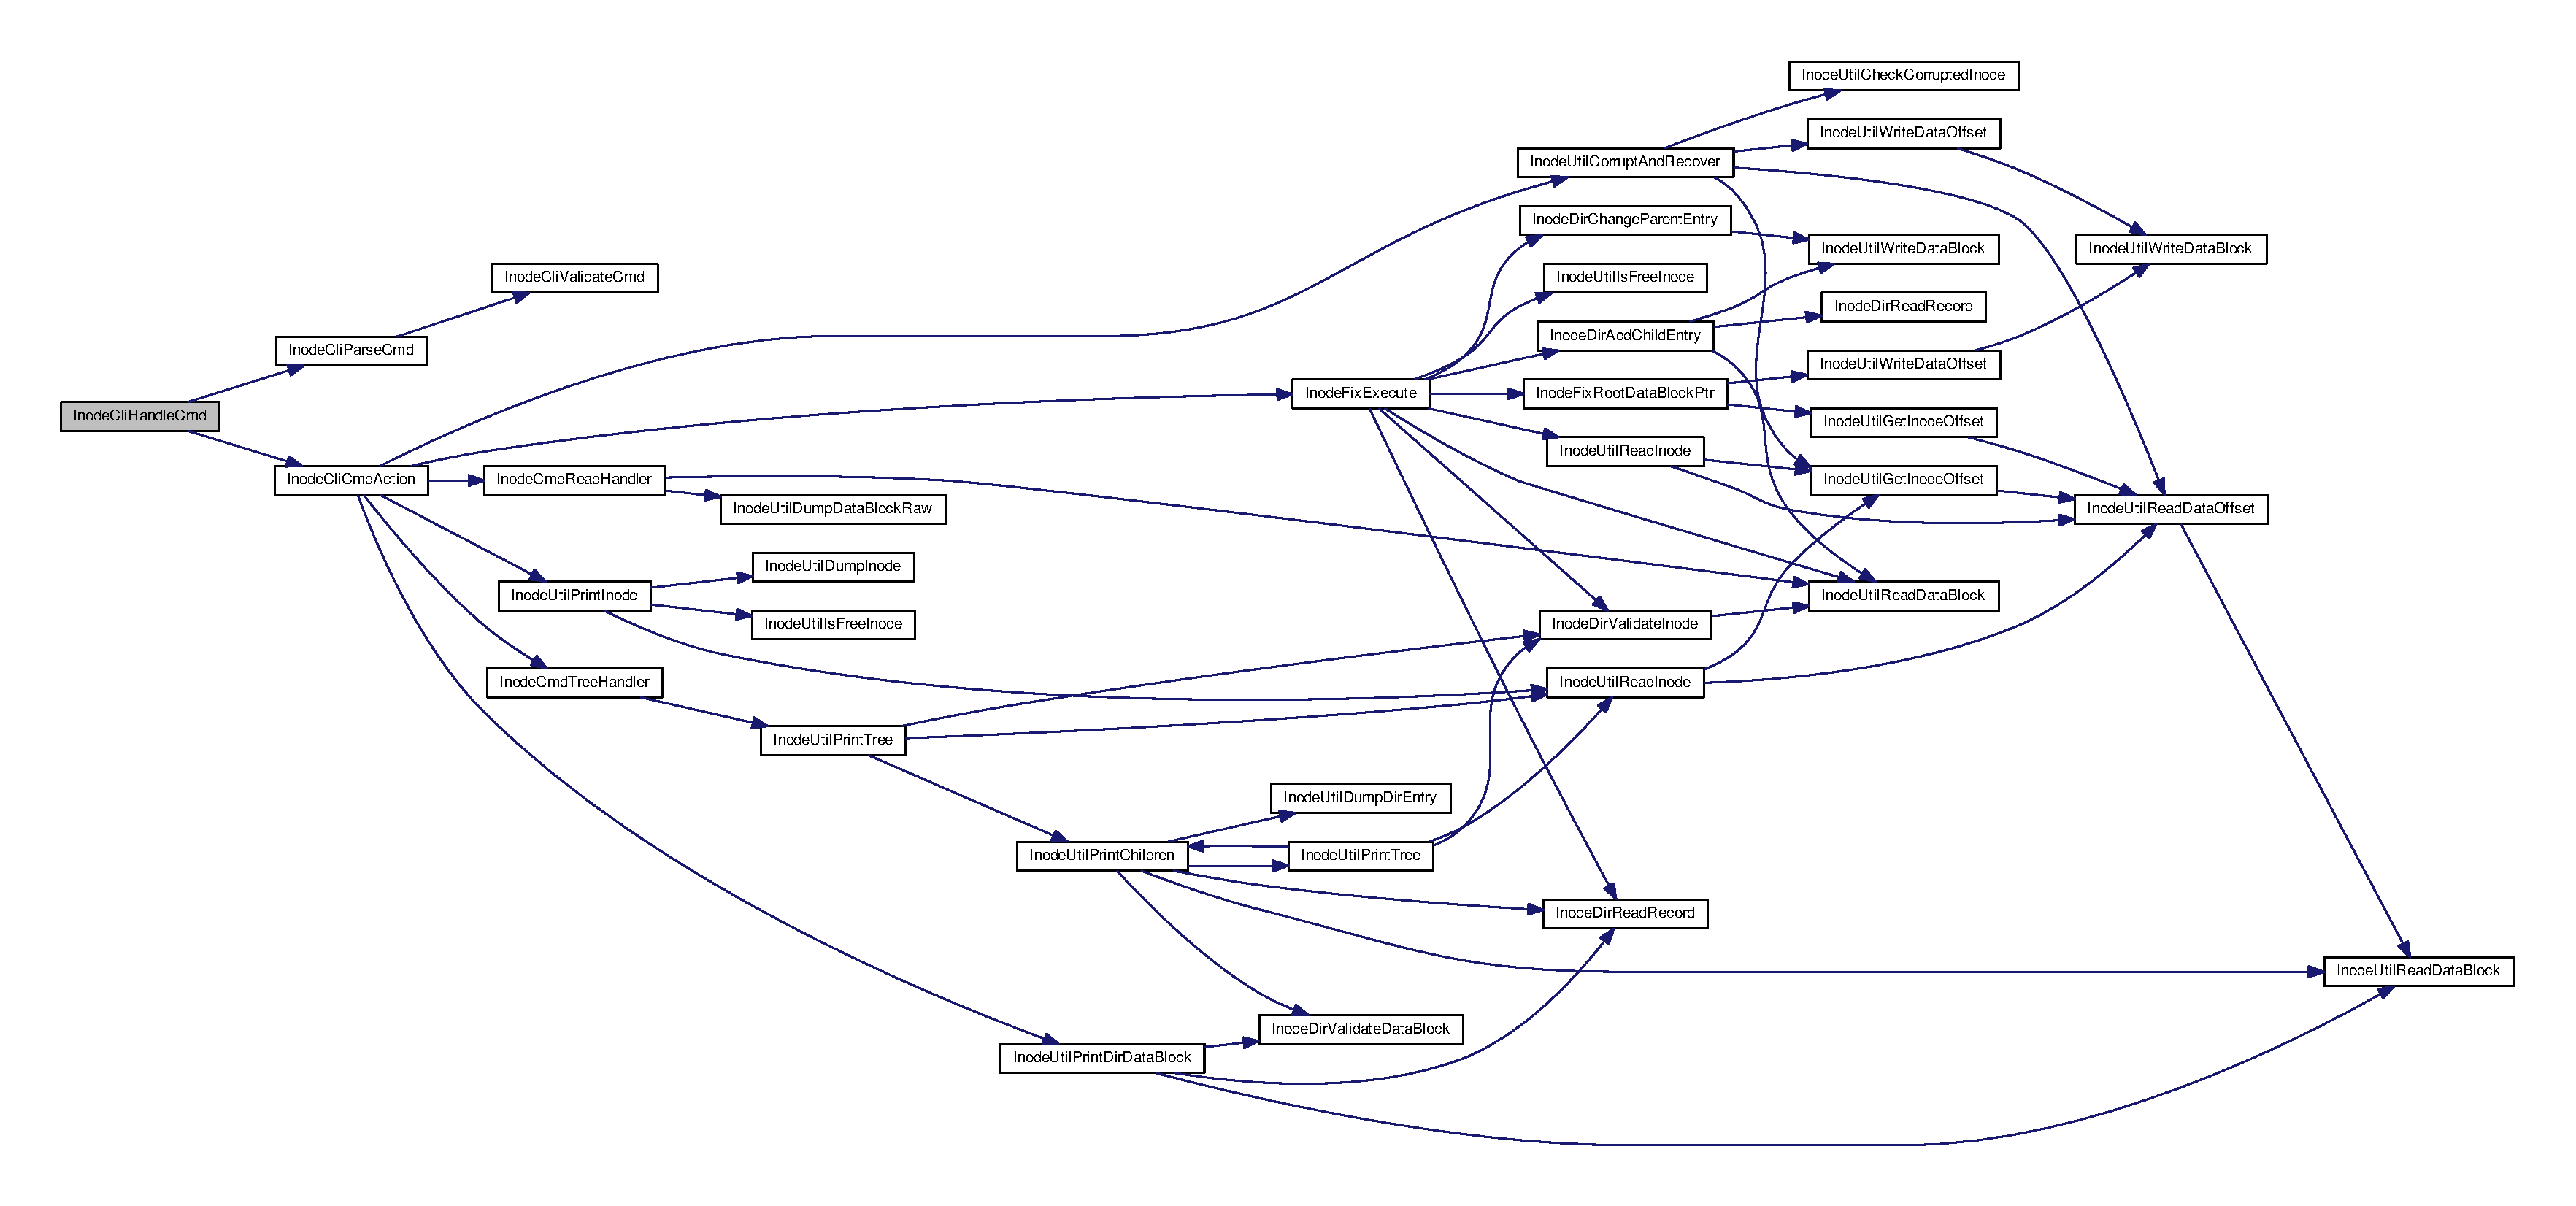
\includegraphics[width=350pt]{inodecli_8c_adde588bd205c9ef530fa02ef8f48cf69_cgraph}
\end{center}
\end{figure}


\hypertarget{inodecli_8c_adaf1a711f6592434c4f1280c0a92fd22}{\index{inodecli.\+c@{inodecli.\+c}!Inode\+Cli\+Parse\+Cmd@{Inode\+Cli\+Parse\+Cmd}}
\index{Inode\+Cli\+Parse\+Cmd@{Inode\+Cli\+Parse\+Cmd}!inodecli.\+c@{inodecli.\+c}}
\subsubsection[{Inode\+Cli\+Parse\+Cmd}]{\setlength{\rightskip}{0pt plus 5cm}I\+N\+T1 Inode\+Cli\+Parse\+Cmd (
\begin{DoxyParamCaption}
\item[{C\+H\+A\+R $\ast$}]{p\+Cmd\+Str, }
\item[{{\bf t\+Command} $\ast$}]{p\+Cmd}
\end{DoxyParamCaption}
)}}\label{inodecli_8c_adaf1a711f6592434c4f1280c0a92fd22}


 Function Name \+: Inode\+Cli\+Parse\+Cmd

Description \+: This Function is used to parse the input command string into the command and arguments.

Input \+: p\+Cmd\+Str -\/ input command string

Output \+: p\+Cmd -\/ structure containing parsed command and arguments

Returns \+: T\+R\+U\+E, if parsing and validation succeeds F\+A\+L\+S\+E otherwise 

Here is the call graph for this function\+:\nopagebreak
\begin{figure}[H]
\begin{center}
\leavevmode
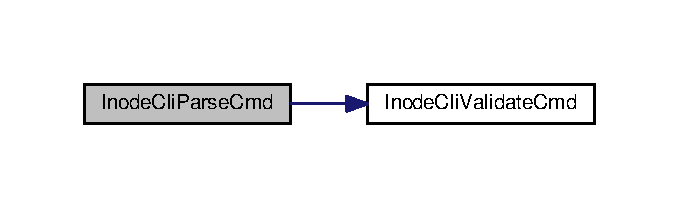
\includegraphics[width=326pt]{inodecli_8c_adaf1a711f6592434c4f1280c0a92fd22_cgraph}
\end{center}
\end{figure}


\hypertarget{inodecli_8c_aa0b53520e1018955fde7aea285159808}{\index{inodecli.\+c@{inodecli.\+c}!Inode\+Cli\+Start@{Inode\+Cli\+Start}}
\index{Inode\+Cli\+Start@{Inode\+Cli\+Start}!inodecli.\+c@{inodecli.\+c}}
\subsubsection[{Inode\+Cli\+Start}]{\setlength{\rightskip}{0pt plus 5cm}V\+O\+I\+D Inode\+Cli\+Start (
\begin{DoxyParamCaption}
{}
\end{DoxyParamCaption}
)}}\label{inodecli_8c_aa0b53520e1018955fde7aea285159808}


 Function Name \+: Inode\+Cli\+Start

Description \+: This Function is used to start the command line interface. This function reads the command input from the user and initiates the action for the command.

Input \+: None

Output \+: None

Returns \+: None 

Here is the call graph for this function\+:\nopagebreak
\begin{figure}[H]
\begin{center}
\leavevmode
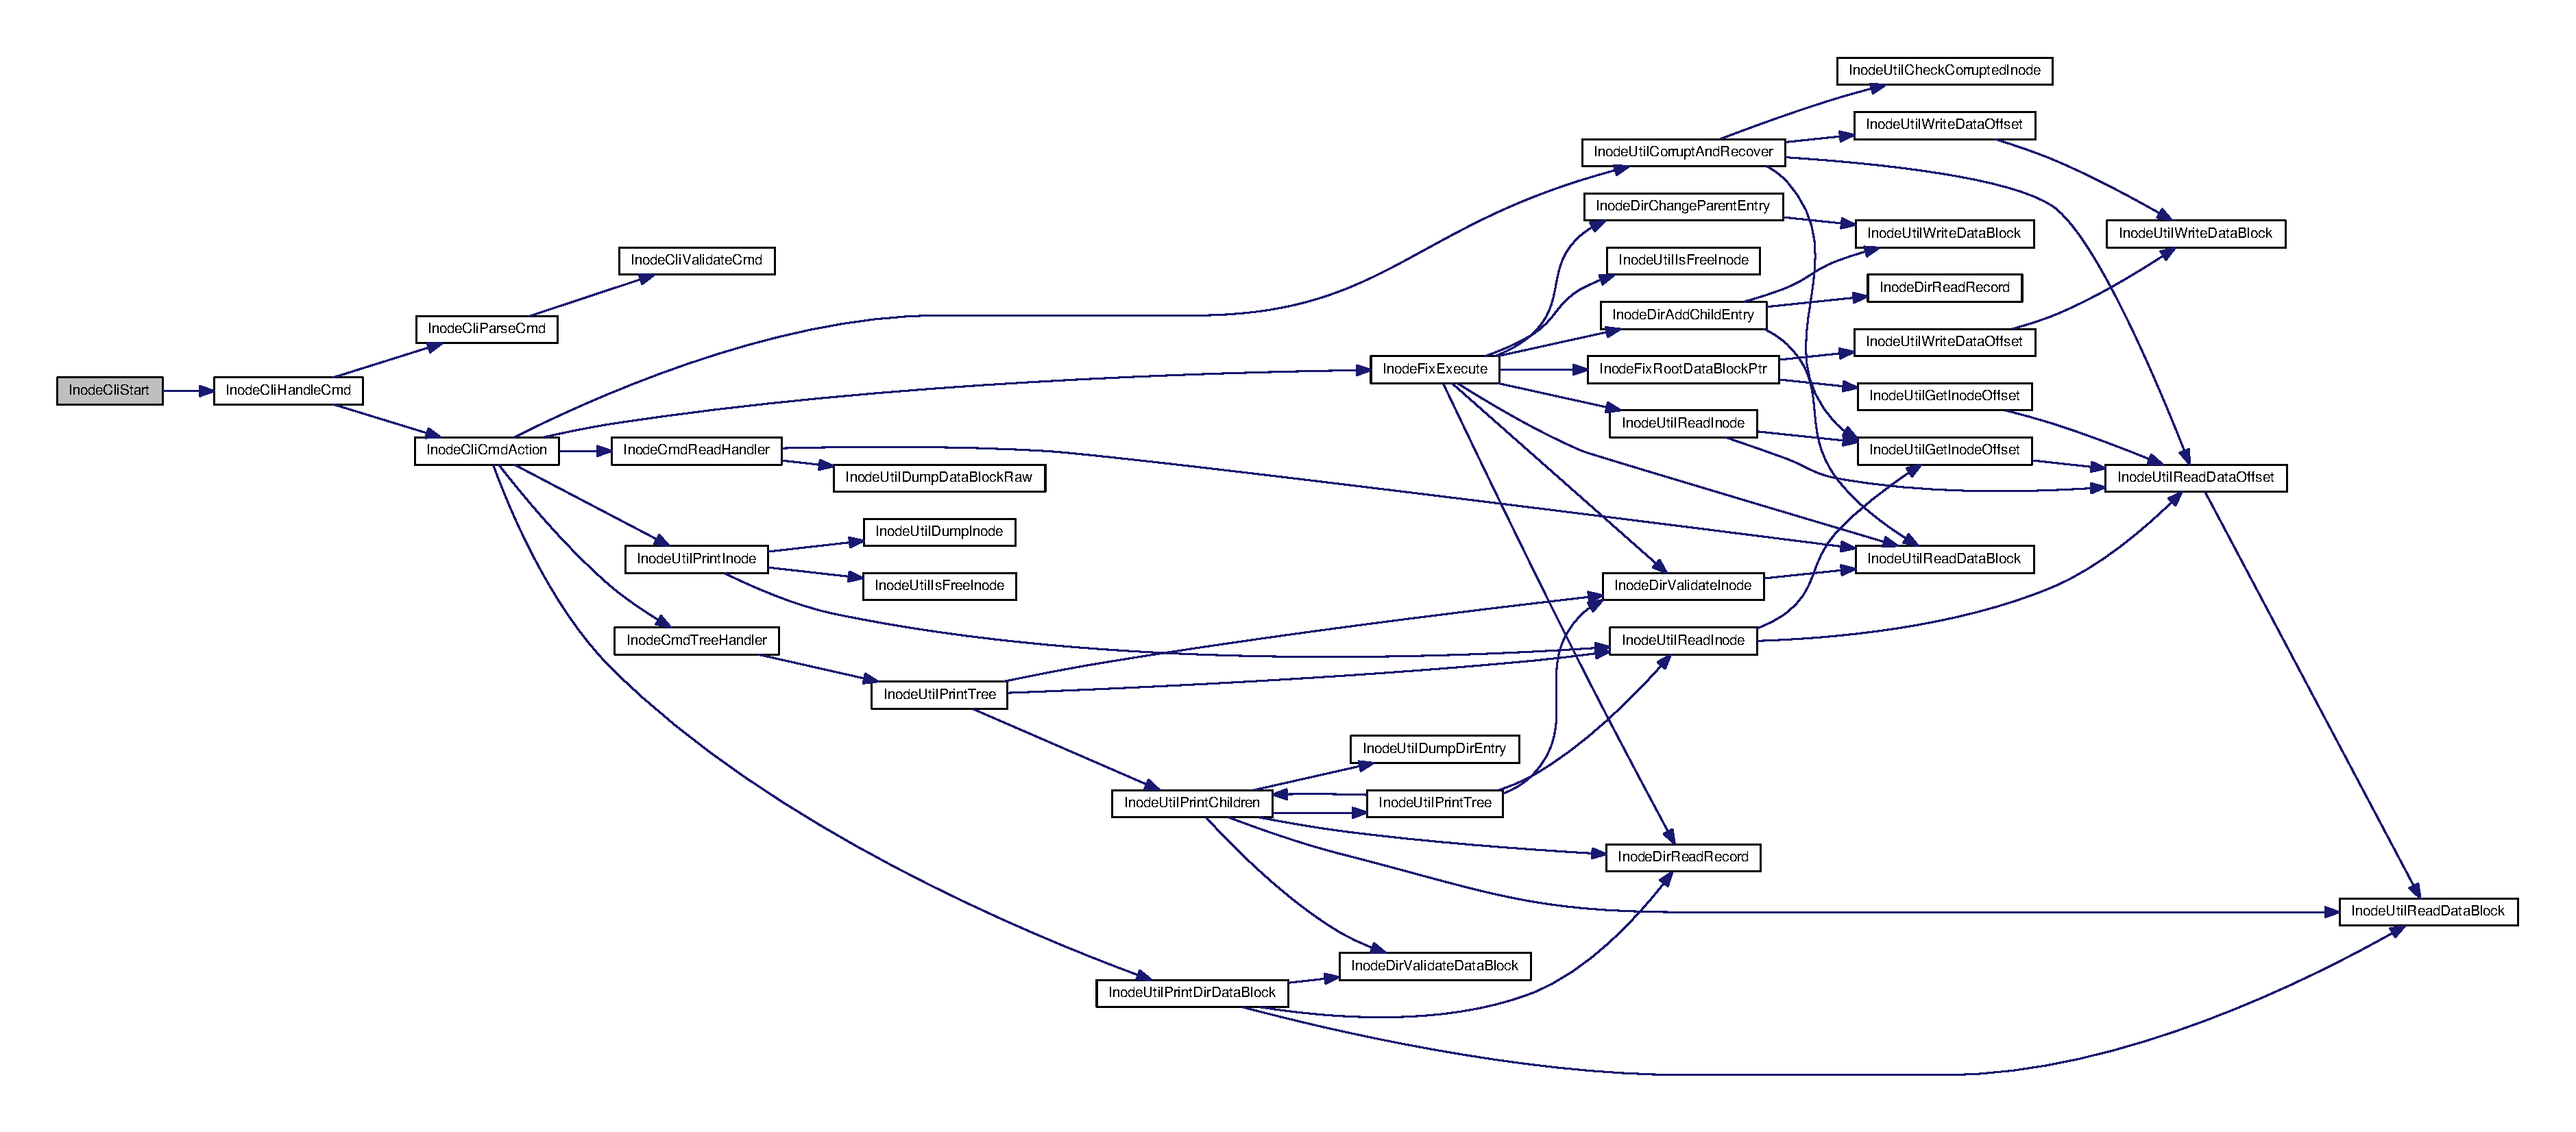
\includegraphics[width=350pt]{inodecli_8c_aa0b53520e1018955fde7aea285159808_cgraph}
\end{center}
\end{figure}


\hypertarget{inodecli_8c_af594f3b863f653a969da942bc1cafe7c}{\index{inodecli.\+c@{inodecli.\+c}!Inode\+Cli\+Validate\+Cmd@{Inode\+Cli\+Validate\+Cmd}}
\index{Inode\+Cli\+Validate\+Cmd@{Inode\+Cli\+Validate\+Cmd}!inodecli.\+c@{inodecli.\+c}}
\subsubsection[{Inode\+Cli\+Validate\+Cmd}]{\setlength{\rightskip}{0pt plus 5cm}I\+N\+T1 Inode\+Cli\+Validate\+Cmd (
\begin{DoxyParamCaption}
\item[{{\bf t\+Command} $\ast$}]{p\+Cmd, }
\item[{U\+I\+N\+T1}]{u1\+Arg\+C}
\end{DoxyParamCaption}
)}}\label{inodecli_8c_af594f3b863f653a969da942bc1cafe7c}


 Function Name \+: Inode\+Cli\+Validate\+Cmd

Description \+: This Function is used to validate the parsed command and arguments

Input \+: p\+Cmd -\/ pointer to the parsed command structure u1\+Arg\+C -\/ no. of arguments in the command input

Output \+: None

Returns \+: T\+R\+U\+E, if validation succeeds F\+A\+L\+S\+E otherwise 

\subsection{Variable Documentation}
\hypertarget{inodecli_8c_a72a268537701a29a14740ed4d190f1f0}{\index{inodecli.\+c@{inodecli.\+c}!g\+Commands@{g\+Commands}}
\index{g\+Commands@{g\+Commands}!inodecli.\+c@{inodecli.\+c}}
\subsubsection[{g\+Commands}]{\setlength{\rightskip}{0pt plus 5cm}{\bf t\+Cmd} g\+Commands\mbox{[}{\bf C\+M\+D\+\_\+\+I\+D\+\_\+\+M\+A\+X}\mbox{]}}}\label{inodecli_8c_a72a268537701a29a14740ed4d190f1f0}
{\bfseries Initial value\+:}
\begin{DoxyCode}
= \{
                \{.Name = \hyperlink{inodecli_8h_a42553adbbb23a03ca876697c00ea44b1}{CMD\_HELP}, .HelpStr = \hyperlink{inodecli_8h_a10620eb7066bd16d02eae9ab03365193}{CMD\_HELP\_HELP}\},
                \{.Name = \hyperlink{inodecli_8h_a4ef842c2bc3e123c98c9379f40a2ab62}{CMD\_CLEAR}, .HelpStr = \hyperlink{inodecli_8h_ad7afbb455c5f2d60f701118f115080d8}{CMD\_CLEAR\_HELP}\},
                \{.Name = \hyperlink{inodecli_8h_acfa1d482ab47b3ceebb9717007111649}{CMD\_EXIT}, .HelpStr = \hyperlink{inodecli_8h_a111d2461881013f301a9f648ac24f601}{CMD\_EXIT\_HELP}\},
                \{.Name = \hyperlink{inodecli_8h_a7391deb9c3a262ded3e186e94eb884e2}{CMD\_WRITE}, .HelpStr = \hyperlink{inodecli_8h_a78cd212696a7b049d87aada2a470c965}{CMD\_WRITE\_HELP}\},
                \{.Name = \hyperlink{inodecli_8h_a286bb7f4b865450f58250d939cf45d90}{CMD\_INODE}, .HelpStr = \hyperlink{inodecli_8h_a7b7763747cb82fcd19aa8dd28e30a071}{CMD\_INODE\_HELP}\},
                \{.Name = \hyperlink{inodecli_8h_a9c953a6c538020e644127ee080608021}{CMD\_READ}, .HelpStr = \hyperlink{inodecli_8h_a03adb8dfb4cdd3faba8978163aaf8c93}{CMD\_READ\_HELP}\},
                \{.Name = \hyperlink{inodecli_8h_a3d2223fa832ff3a2aeb97888ce9856f9}{CMD\_DIR}, .HelpStr = \hyperlink{inodecli_8h_a5474da458a635be412d5704a02f0df83}{CMD\_DIR\_HELP}\},
                \{.Name = \hyperlink{inodecli_8h_a7517d4f10c0034f27827f5cfe77cf52a}{CMD\_TREE}, .HelpStr = \hyperlink{inodecli_8h_a9008063814b97ecefc54f5a46e19b340}{CMD\_TREE\_HELP}\},
                \{.Name = \hyperlink{inodecli_8h_a430ac043851c4efc20762af91d89f7b9}{CMD\_CORRUPT}, .HelpStr = \hyperlink{inodecli_8h_a57a92b33d047525dc9e69eb72de6269e}{CMD\_CORRUPT\_HELP}\},
                \{.Name = \hyperlink{inodecli_8h_a68980ecdee8879dfba5618de489ca766}{CMD\_FIX}, .HelpStr = \hyperlink{inodecli_8h_af2e6404e0cf07b14693e23d54937f010}{CMD\_FIX\_HELP}\},
                \{.Name = \hyperlink{inodecli_8h_aebfe91c6148b6492ffab5cdd7ced8b70}{CMD\_RECOVER}, .HelpStr = \hyperlink{inodecli_8h_ab151080fd3feb4380a5bd65353ce60d5}{CMD\_RECOVER\_HELP}\},
                
                \}
\end{DoxyCode}
\hypertarget{inodecli_8c_ac732f1e6c26e35b8e7fbb38498b415e4}{\index{inodecli.\+c@{inodecli.\+c}!gu1\+Exit@{gu1\+Exit}}
\index{gu1\+Exit@{gu1\+Exit}!inodecli.\+c@{inodecli.\+c}}
\subsubsection[{gu1\+Exit}]{\setlength{\rightskip}{0pt plus 5cm}U\+I\+N\+T1 gu1\+Exit}}\label{inodecli_8c_ac732f1e6c26e35b8e7fbb38498b415e4}

\hypertarget{inodecmd_8c}{\section{src/inodecmd.c File Reference}
\label{inodecmd_8c}\index{src/inodecmd.\+c@{src/inodecmd.\+c}}
}
{\ttfamily \#include \char`\"{}inodeinc.\+h\char`\"{}}\\*
Include dependency graph for inodecmd.\+c\+:\nopagebreak
\begin{figure}[H]
\begin{center}
\leavevmode
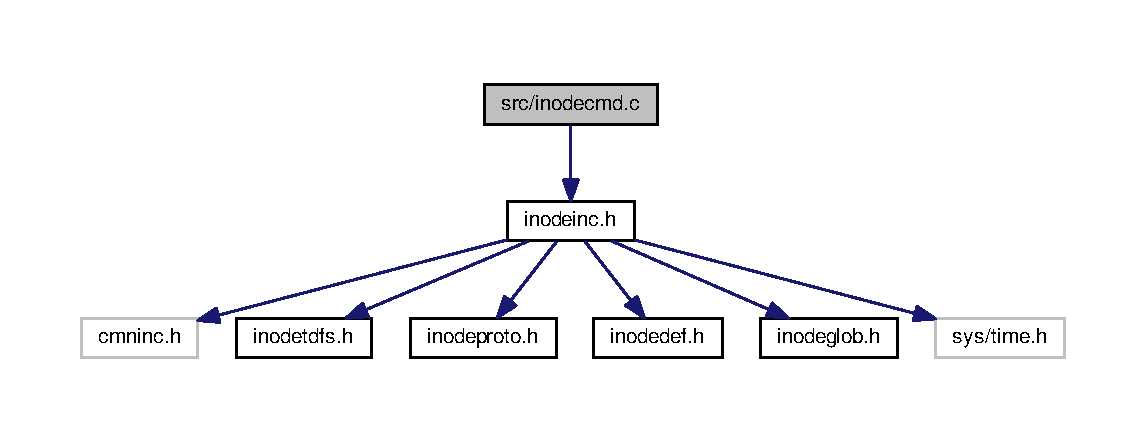
\includegraphics[width=350pt]{inodecmd_8c__incl}
\end{center}
\end{figure}
\subsection*{Functions}
\begin{DoxyCompactItemize}
\item 
V\+O\+I\+D \hyperlink{inodecmd_8c_a2ea2fdd045177335a3a2f8cd89678cb9}{Inode\+Cmd\+Tree\+Handler} (U\+I\+N\+T4 u4\+Inode\+No)
\item 
V\+O\+I\+D \hyperlink{inodecmd_8c_a1635e6bd723f78d1355e30c815348a34}{Inode\+Cmd\+Read\+Handler} (U\+I\+N\+T4 u4\+Block\+No)
\end{DoxyCompactItemize}


\subsection{Function Documentation}
\hypertarget{inodecmd_8c_a1635e6bd723f78d1355e30c815348a34}{\index{inodecmd.\+c@{inodecmd.\+c}!Inode\+Cmd\+Read\+Handler@{Inode\+Cmd\+Read\+Handler}}
\index{Inode\+Cmd\+Read\+Handler@{Inode\+Cmd\+Read\+Handler}!inodecmd.\+c@{inodecmd.\+c}}
\subsubsection[{Inode\+Cmd\+Read\+Handler}]{\setlength{\rightskip}{0pt plus 5cm}V\+O\+I\+D Inode\+Cmd\+Read\+Handler (
\begin{DoxyParamCaption}
\item[{U\+I\+N\+T4}]{u4\+Block\+No}
\end{DoxyParamCaption}
)}}\label{inodecmd_8c_a1635e6bd723f78d1355e30c815348a34}


 Function Name \+: Inode\+Cmd\+Read\+Handler

Description \+: This is the handler function for the command 'read'. This function reads the block specified and prints the contents in H\+E\+X.

Input \+: u4\+Block\+No -\/ Block number to read.

Output \+: None

Returns \+: None 

Here is the call graph for this function\+:\nopagebreak
\begin{figure}[H]
\begin{center}
\leavevmode
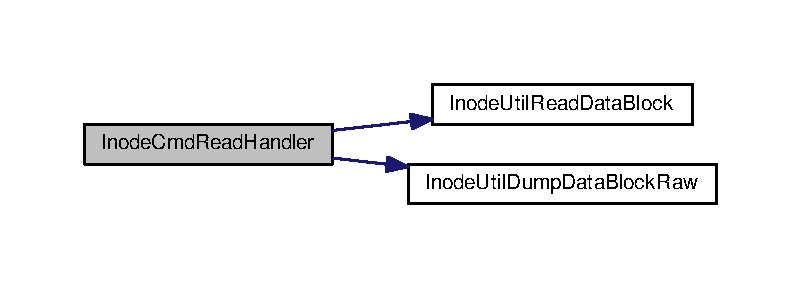
\includegraphics[width=350pt]{inodecmd_8c_a1635e6bd723f78d1355e30c815348a34_cgraph}
\end{center}
\end{figure}


\hypertarget{inodecmd_8c_a2ea2fdd045177335a3a2f8cd89678cb9}{\index{inodecmd.\+c@{inodecmd.\+c}!Inode\+Cmd\+Tree\+Handler@{Inode\+Cmd\+Tree\+Handler}}
\index{Inode\+Cmd\+Tree\+Handler@{Inode\+Cmd\+Tree\+Handler}!inodecmd.\+c@{inodecmd.\+c}}
\subsubsection[{Inode\+Cmd\+Tree\+Handler}]{\setlength{\rightskip}{0pt plus 5cm}V\+O\+I\+D Inode\+Cmd\+Tree\+Handler (
\begin{DoxyParamCaption}
\item[{U\+I\+N\+T4}]{u4\+Inode\+No}
\end{DoxyParamCaption}
)}}\label{inodecmd_8c_a2ea2fdd045177335a3a2f8cd89678cb9}


 Function Name \+: Inode\+Cmd\+Tree\+Handler

Description \+: This is the handler function for the command 'tree'. This function prints the directory/files tree starting at the given inode.

Input \+: u4\+Inode\+No -\/ Root inode to start.

Output \+: None

Returns \+: None 

Here is the call graph for this function\+:\nopagebreak
\begin{figure}[H]
\begin{center}
\leavevmode
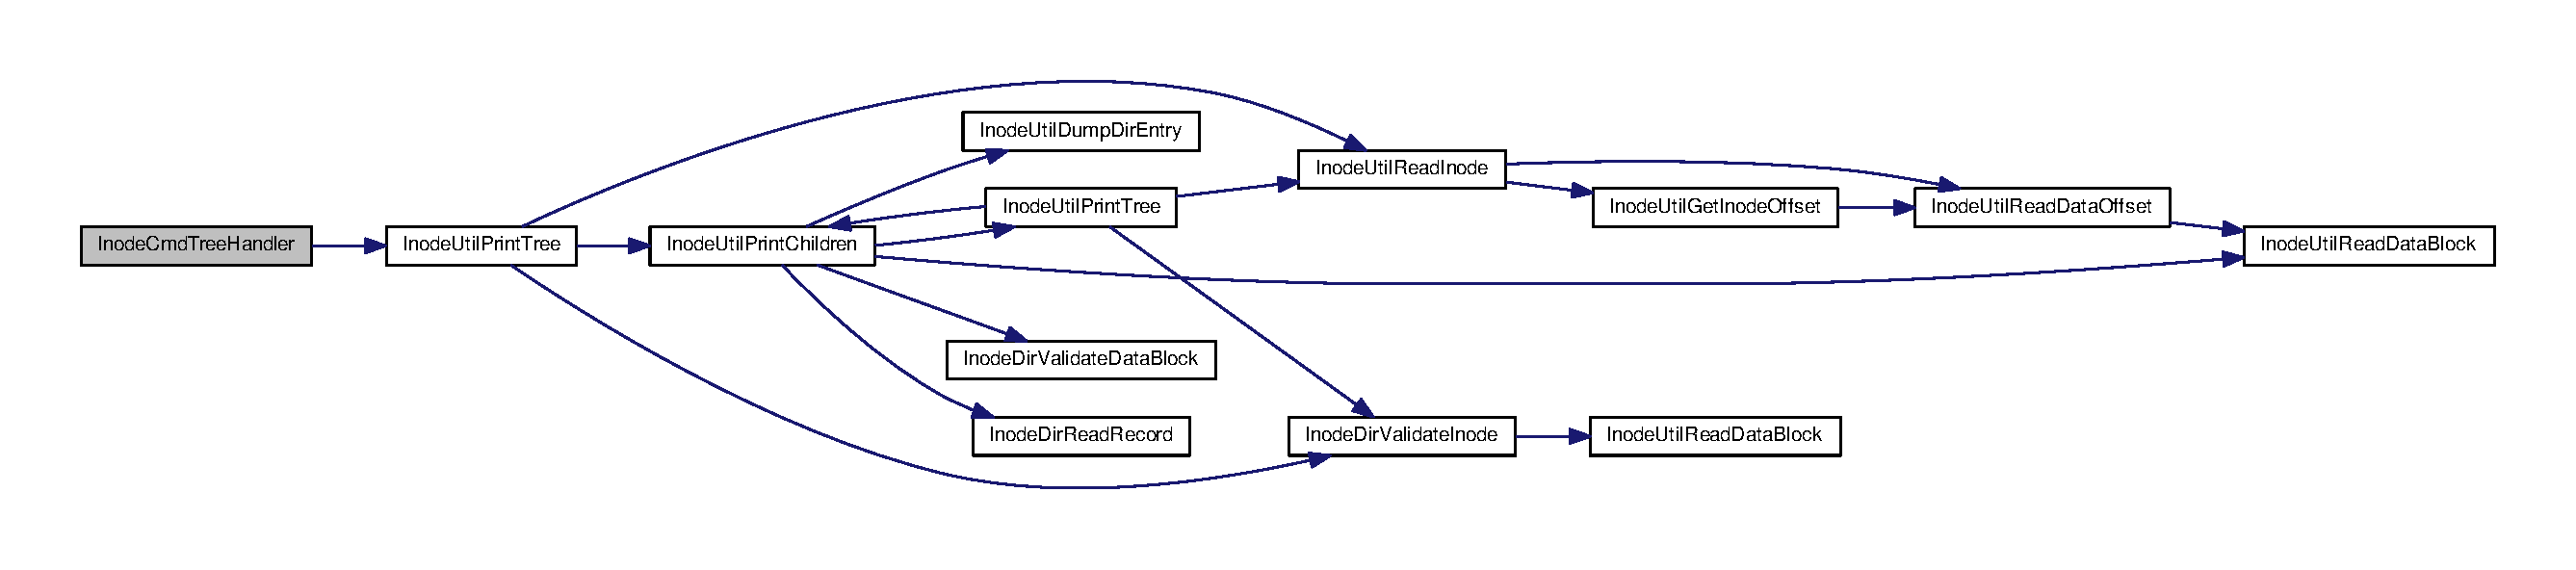
\includegraphics[width=350pt]{inodecmd_8c_a2ea2fdd045177335a3a2f8cd89678cb9_cgraph}
\end{center}
\end{figure}



\hypertarget{inodedir_8c}{\section{src/inodedir.c File Reference}
\label{inodedir_8c}\index{src/inodedir.\+c@{src/inodedir.\+c}}
}
{\ttfamily \#include \char`\"{}inodeinc.\+h\char`\"{}}\\*
Include dependency graph for inodedir.\+c\+:\nopagebreak
\begin{figure}[H]
\begin{center}
\leavevmode
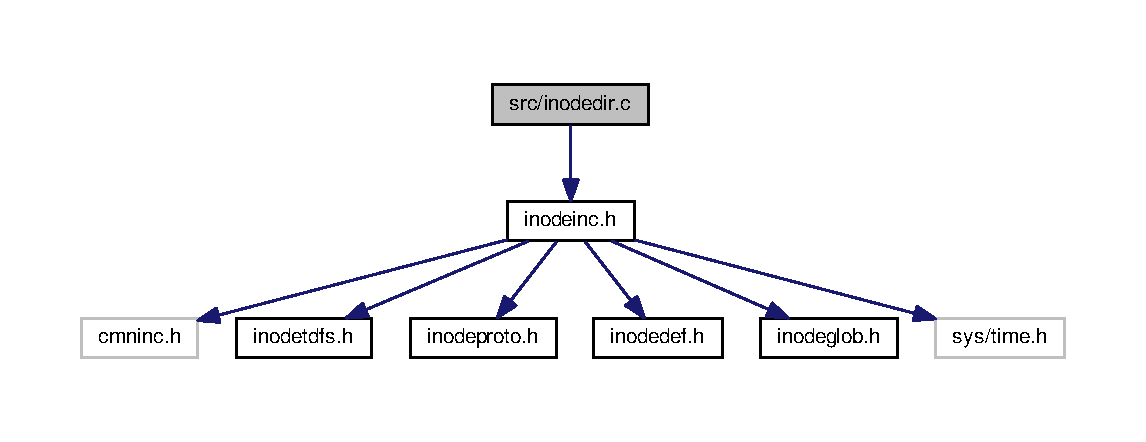
\includegraphics[width=350pt]{inodedir_8c__incl}
\end{center}
\end{figure}
\subsection*{Functions}
\begin{DoxyCompactItemize}
\item 
I\+N\+T4 \hyperlink{inodedir_8c_a648f1f0adeeb821396ff675be7ce3a0a}{Inode\+Dir\+Validate\+Inode} (U\+I\+N\+T4 u4\+Inode\+No, U\+I\+N\+T4 u4\+Block\+No)
\item 
I\+N\+T4 \hyperlink{inodedir_8c_a9513ab1ee8f7fcc872a1f5c14af8a985}{Inode\+Dir\+Read\+Record} (C\+H\+A\+R $\ast$p\+Entries, U\+I\+N\+T4 u4\+Start\+Pos, struct ext3\+\_\+dir\+\_\+entry\+\_\+2 $\ast$p\+Dir\+Entry)
\item 
I\+N\+T4 \hyperlink{inodedir_8c_a90a015688692be14fcbf9ad6f52b24b2}{Inode\+Dir\+Validate\+Data\+Block} (C\+H\+A\+R $\ast$p\+Entries)
\item 
I\+N\+T4 \hyperlink{inodedir_8c_a89c0632678345a3ec36ec25c31872df4}{Inode\+Dir\+Change\+Parent\+Entry} (struct ext3\+\_\+dir\+\_\+entry\+\_\+2 $\ast$p\+Dir\+Entry, U\+I\+N\+T4 u4\+Block\+No)
\item 
I\+N\+T4 \hyperlink{inodedir_8c_ab78d127da1b1fe403246e840bd3862eb}{Inode\+Dir\+Add\+Child\+Entry} (struct ext3\+\_\+dir\+\_\+entry\+\_\+2 $\ast$p\+New\+Child, U\+I\+N\+T4 u4\+Block\+No)
\end{DoxyCompactItemize}


\subsection{Function Documentation}
\hypertarget{inodedir_8c_ab78d127da1b1fe403246e840bd3862eb}{\index{inodedir.\+c@{inodedir.\+c}!Inode\+Dir\+Add\+Child\+Entry@{Inode\+Dir\+Add\+Child\+Entry}}
\index{Inode\+Dir\+Add\+Child\+Entry@{Inode\+Dir\+Add\+Child\+Entry}!inodedir.\+c@{inodedir.\+c}}
\subsubsection[{Inode\+Dir\+Add\+Child\+Entry}]{\setlength{\rightskip}{0pt plus 5cm}I\+N\+T4 Inode\+Dir\+Add\+Child\+Entry (
\begin{DoxyParamCaption}
\item[{struct ext3\+\_\+dir\+\_\+entry\+\_\+2 $\ast$}]{p\+New\+Child, }
\item[{U\+I\+N\+T4}]{u4\+Block\+No}
\end{DoxyParamCaption}
)}}\label{inodedir_8c_ab78d127da1b1fe403246e840bd3862eb}


 Function Name \+: Inode\+Dir\+Add\+Child\+Entry

Author \+: Anusha Seshadri

Description \+: This Function is used to add a child entry to a directory inode. The new entry would be appended at the end of the last entry.

Input \+: p\+Dir\+Entry -\/ new child entry u4\+Block\+No -\/ the directory data block where the child entry needs to be changed Output \+: None

Returns \+: I\+N\+O\+D\+E\+\_\+\+S\+U\+C\+C\+E\+S\+S, if the child entry is addded successfully I\+N\+O\+D\+E\+\_\+\+F\+A\+I\+L\+U\+R\+E otherwise 

Here is the call graph for this function\+:\nopagebreak
\begin{figure}[H]
\begin{center}
\leavevmode
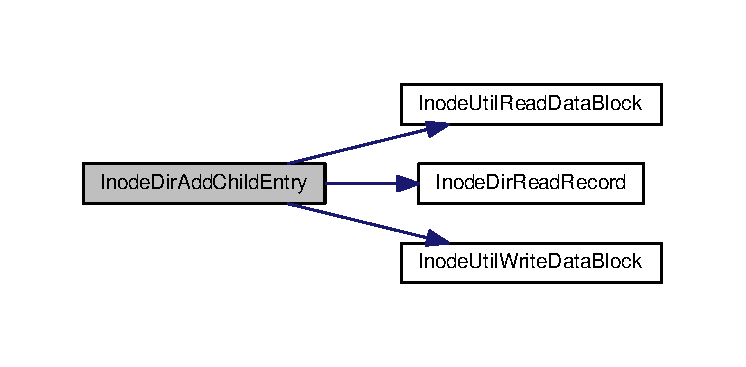
\includegraphics[width=350pt]{inodedir_8c_ab78d127da1b1fe403246e840bd3862eb_cgraph}
\end{center}
\end{figure}


\hypertarget{inodedir_8c_a89c0632678345a3ec36ec25c31872df4}{\index{inodedir.\+c@{inodedir.\+c}!Inode\+Dir\+Change\+Parent\+Entry@{Inode\+Dir\+Change\+Parent\+Entry}}
\index{Inode\+Dir\+Change\+Parent\+Entry@{Inode\+Dir\+Change\+Parent\+Entry}!inodedir.\+c@{inodedir.\+c}}
\subsubsection[{Inode\+Dir\+Change\+Parent\+Entry}]{\setlength{\rightskip}{0pt plus 5cm}I\+N\+T4 Inode\+Dir\+Change\+Parent\+Entry (
\begin{DoxyParamCaption}
\item[{struct ext3\+\_\+dir\+\_\+entry\+\_\+2 $\ast$}]{p\+Dir\+Entry, }
\item[{U\+I\+N\+T4}]{u4\+Block\+No}
\end{DoxyParamCaption}
)}}\label{inodedir_8c_a89c0632678345a3ec36ec25c31872df4}


 Function Name \+: Inode\+Dir\+Change\+Parent\+Entry

Author \+: Anusha Seshadri

Description \+: This Function is used to change the parent directory entry of a directory inode.

Input \+: p\+Dir\+Entry -\/ new parent entry u4\+Block\+No -\/ the directory data block where the parent entry needs to be changed Output \+: None

Returns \+: I\+N\+O\+D\+E\+\_\+\+S\+U\+C\+C\+E\+S\+S, if the parent is changed successfully I\+N\+O\+D\+E\+\_\+\+F\+A\+I\+L\+U\+R\+E otherwise 

Here is the call graph for this function\+:\nopagebreak
\begin{figure}[H]
\begin{center}
\leavevmode
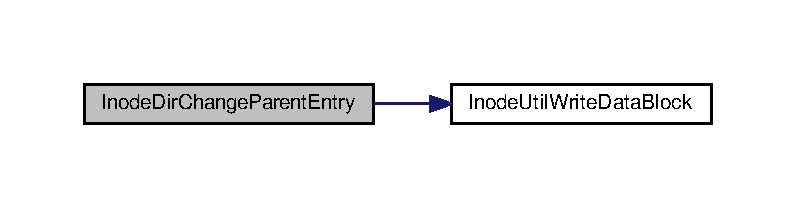
\includegraphics[width=350pt]{inodedir_8c_a89c0632678345a3ec36ec25c31872df4_cgraph}
\end{center}
\end{figure}


\hypertarget{inodedir_8c_a9513ab1ee8f7fcc872a1f5c14af8a985}{\index{inodedir.\+c@{inodedir.\+c}!Inode\+Dir\+Read\+Record@{Inode\+Dir\+Read\+Record}}
\index{Inode\+Dir\+Read\+Record@{Inode\+Dir\+Read\+Record}!inodedir.\+c@{inodedir.\+c}}
\subsubsection[{Inode\+Dir\+Read\+Record}]{\setlength{\rightskip}{0pt plus 5cm}I\+N\+T4 Inode\+Dir\+Read\+Record (
\begin{DoxyParamCaption}
\item[{C\+H\+A\+R $\ast$}]{p\+Entries, }
\item[{U\+I\+N\+T4}]{u4\+Start\+Pos, }
\item[{struct ext3\+\_\+dir\+\_\+entry\+\_\+2 $\ast$}]{p\+Dir\+Entry}
\end{DoxyParamCaption}
)}}\label{inodedir_8c_a9513ab1ee8f7fcc872a1f5c14af8a985}


 Function Name \+: Inode\+Dir\+Read\+Record

Author \+: Naveen Raj Selvaraj

Description \+: This Function is used to read a directory entry from the data block of a directory inode.

Input \+: p\+Entries -\/ Buffer containing the contents of the data block u4\+Start\+Pos -\/ Offset to start reading

Output \+: p\+Dir\+Entry -\/ the directory entry read from the block

Returns \+: I\+N\+O\+D\+E\+\_\+\+S\+U\+C\+C\+E\+S\+S, if the entry is read successfully I\+N\+O\+D\+E\+\_\+\+F\+A\+I\+L\+U\+R\+E otherwise \hypertarget{inodedir_8c_a90a015688692be14fcbf9ad6f52b24b2}{\index{inodedir.\+c@{inodedir.\+c}!Inode\+Dir\+Validate\+Data\+Block@{Inode\+Dir\+Validate\+Data\+Block}}
\index{Inode\+Dir\+Validate\+Data\+Block@{Inode\+Dir\+Validate\+Data\+Block}!inodedir.\+c@{inodedir.\+c}}
\subsubsection[{Inode\+Dir\+Validate\+Data\+Block}]{\setlength{\rightskip}{0pt plus 5cm}I\+N\+T4 Inode\+Dir\+Validate\+Data\+Block (
\begin{DoxyParamCaption}
\item[{C\+H\+A\+R $\ast$}]{p\+Entries}
\end{DoxyParamCaption}
)}}\label{inodedir_8c_a90a015688692be14fcbf9ad6f52b24b2}


 Function Name \+: Inode\+Dir\+Validate\+Data\+Block

Author \+: Naveen Raj Selvaraj

Description \+: This Function is used to check if a data block is a directory data block or not. If the data block contains directory entries, then it is a valid directory data block.

Input \+: p\+Entries -\/ Buffer containing the contents of the data block Output \+: None

Returns \+: I\+N\+O\+D\+E\+\_\+\+S\+U\+C\+C\+E\+S\+S, if the data block is a valid directory data block I\+N\+O\+D\+E\+\_\+\+F\+A\+I\+L\+U\+R\+E otherwise \hypertarget{inodedir_8c_a648f1f0adeeb821396ff675be7ce3a0a}{\index{inodedir.\+c@{inodedir.\+c}!Inode\+Dir\+Validate\+Inode@{Inode\+Dir\+Validate\+Inode}}
\index{Inode\+Dir\+Validate\+Inode@{Inode\+Dir\+Validate\+Inode}!inodedir.\+c@{inodedir.\+c}}
\subsubsection[{Inode\+Dir\+Validate\+Inode}]{\setlength{\rightskip}{0pt plus 5cm}I\+N\+T4 Inode\+Dir\+Validate\+Inode (
\begin{DoxyParamCaption}
\item[{U\+I\+N\+T4}]{u4\+Inode\+No, }
\item[{U\+I\+N\+T4}]{u4\+Block\+No}
\end{DoxyParamCaption}
)}}\label{inodedir_8c_a648f1f0adeeb821396ff675be7ce3a0a}


 Function Name \+: Inode\+Dir\+Validate\+Inode

Author \+: Naveen Raj Selvaraj

Description \+: This Function is used to validate a directory inode. A directory inode is valid if the data block pointer points to the actual data block of inode. If the data block pointer is corrupted, then the directory inode is invalid.

Input \+: u4\+Inode\+No -\/ Directory Inode number u4\+Block\+No -\/ data block pointed by the inode's first direct block pointer Output \+: None

Returns \+: I\+N\+O\+D\+E\+\_\+\+S\+U\+C\+C\+E\+S\+S, if the inode is a valid directory inode I\+N\+O\+D\+E\+\_\+\+F\+A\+I\+L\+U\+R\+E otherwise 

Here is the call graph for this function\+:\nopagebreak
\begin{figure}[H]
\begin{center}
\leavevmode
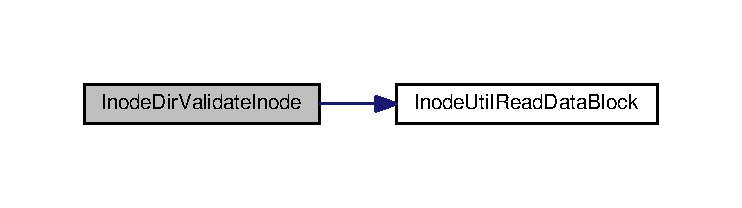
\includegraphics[width=350pt]{inodedir_8c_a648f1f0adeeb821396ff675be7ce3a0a_cgraph}
\end{center}
\end{figure}



\hypertarget{inodefix_8c}{\section{src/inodefix.c File Reference}
\label{inodefix_8c}\index{src/inodefix.\+c@{src/inodefix.\+c}}
}
{\ttfamily \#include \char`\"{}inodeinc.\+h\char`\"{}}\\*
{\ttfamily \#include \char`\"{}inodetime.\+h\char`\"{}}\\*
Include dependency graph for inodefix.\+c\+:\nopagebreak
\begin{figure}[H]
\begin{center}
\leavevmode
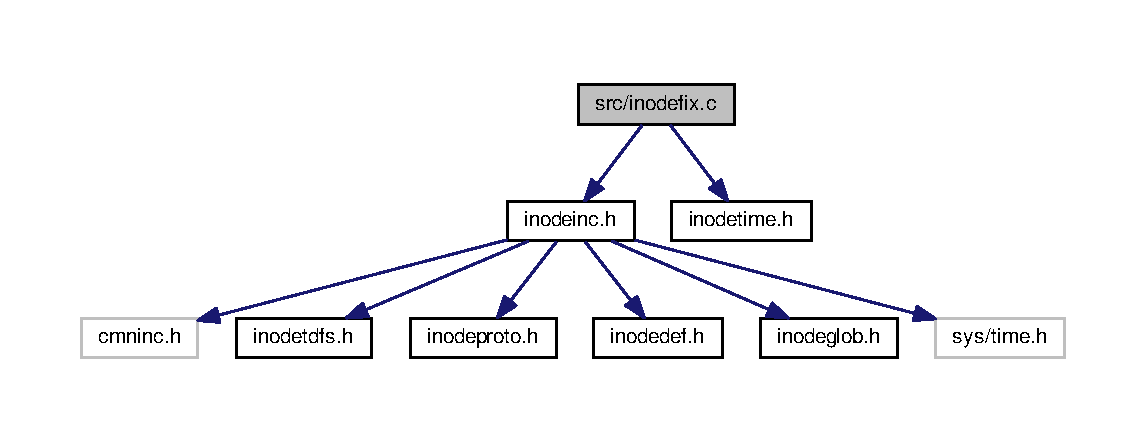
\includegraphics[width=350pt]{inodefix_8c__incl}
\end{center}
\end{figure}
\subsection*{Functions}
\begin{DoxyCompactItemize}
\item 
I\+N\+T4 \hyperlink{inodefix_8c_a0cf855704a34cb63b52487e75b12052c}{Inode\+Fix\+Execute} ()
\item 
I\+N\+T4 \hyperlink{inodefix_8c_adbd08c2df1e429581a73b0ffd6108cb6}{Inode\+Fix\+Root\+Data\+Block\+Ptr} (struct ext3\+\_\+inode $\ast$p\+Inode)
\end{DoxyCompactItemize}


\subsection{Function Documentation}
\hypertarget{inodefix_8c_a0cf855704a34cb63b52487e75b12052c}{\index{inodefix.\+c@{inodefix.\+c}!Inode\+Fix\+Execute@{Inode\+Fix\+Execute}}
\index{Inode\+Fix\+Execute@{Inode\+Fix\+Execute}!inodefix.\+c@{inodefix.\+c}}
\subsubsection[{Inode\+Fix\+Execute}]{\setlength{\rightskip}{0pt plus 5cm}I\+N\+T4 Inode\+Fix\+Execute (
\begin{DoxyParamCaption}
{}
\end{DoxyParamCaption}
)}}\label{inodefix_8c_a0cf855704a34cb63b52487e75b12052c}


 Function Name \+: Inode\+Fix\+Execute

Description \+: This Function is used to recover the corrupted directories children directories. Please refer the documentation for the recovery algorithm.

Input \+: None

Output \+: None

Returns \+: I\+N\+O\+D\+E\+\_\+\+S\+U\+C\+C\+E\+S\+S, on successful recovery I\+N\+O\+D\+E\+\_\+\+F\+A\+I\+L\+U\+R\+E otherwise 

Here is the call graph for this function\+:\nopagebreak
\begin{figure}[H]
\begin{center}
\leavevmode
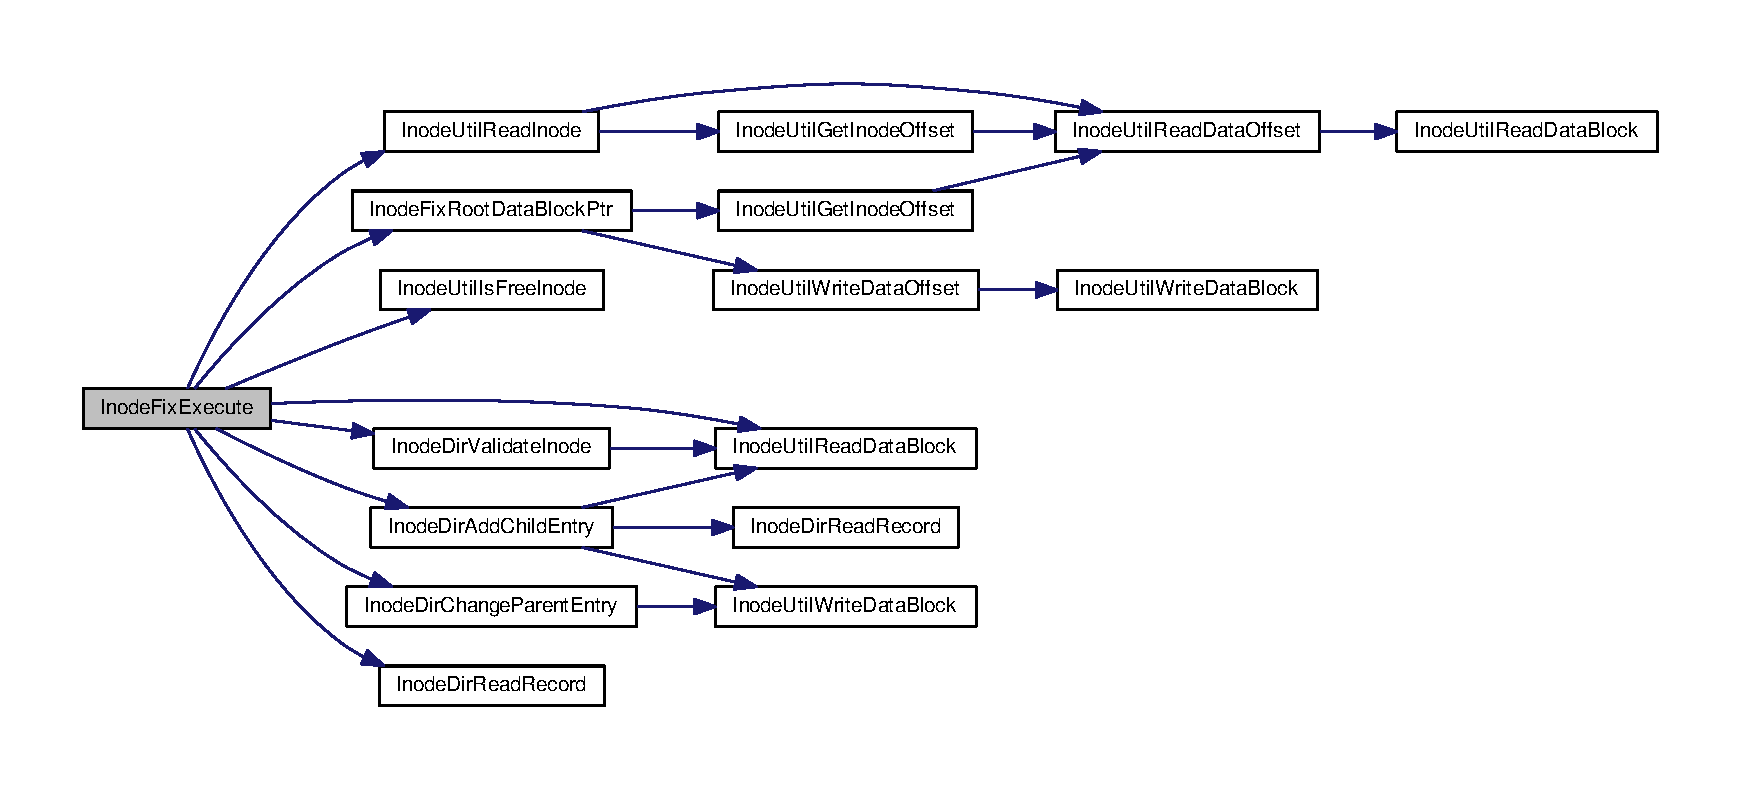
\includegraphics[width=350pt]{inodefix_8c_a0cf855704a34cb63b52487e75b12052c_cgraph}
\end{center}
\end{figure}


\hypertarget{inodefix_8c_adbd08c2df1e429581a73b0ffd6108cb6}{\index{inodefix.\+c@{inodefix.\+c}!Inode\+Fix\+Root\+Data\+Block\+Ptr@{Inode\+Fix\+Root\+Data\+Block\+Ptr}}
\index{Inode\+Fix\+Root\+Data\+Block\+Ptr@{Inode\+Fix\+Root\+Data\+Block\+Ptr}!inodefix.\+c@{inodefix.\+c}}
\subsubsection[{Inode\+Fix\+Root\+Data\+Block\+Ptr}]{\setlength{\rightskip}{0pt plus 5cm}I\+N\+T4 Inode\+Fix\+Root\+Data\+Block\+Ptr (
\begin{DoxyParamCaption}
\item[{struct ext3\+\_\+inode $\ast$}]{p\+Inode}
\end{DoxyParamCaption}
)}}\label{inodefix_8c_adbd08c2df1e429581a73b0ffd6108cb6}


 Function Name \+: Inode\+Fix\+Root\+Data\+Block\+Ptr

Description \+: This Function is used to fix the root inode's data block pointer if it is corrupted.

Input \+: p\+Inode -\/ Root Inode structure

Output \+: None

Returns \+: I\+N\+O\+D\+E\+\_\+\+S\+U\+C\+C\+E\+S\+S, if the data block pointer is fixed I\+N\+O\+D\+E\+\_\+\+F\+A\+I\+L\+U\+R\+E otherwise 

Here is the call graph for this function\+:\nopagebreak
\begin{figure}[H]
\begin{center}
\leavevmode
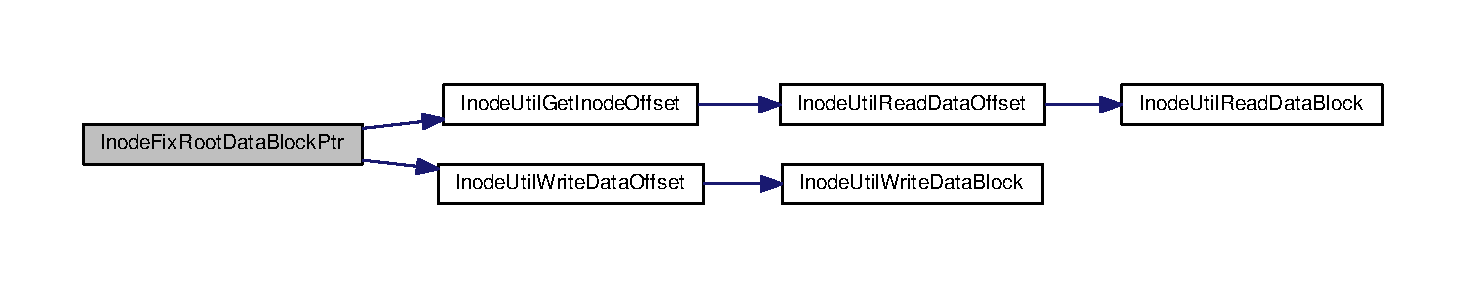
\includegraphics[width=350pt]{inodefix_8c_adbd08c2df1e429581a73b0ffd6108cb6_cgraph}
\end{center}
\end{figure}



\hypertarget{inodeinit_8c}{\section{src/inodeinit.c File Reference}
\label{inodeinit_8c}\index{src/inodeinit.\+c@{src/inodeinit.\+c}}
}
{\ttfamily \#include \char`\"{}inodeinc.\+h\char`\"{}}\\*
{\ttfamily \#include $<$errno.\+h$>$}\\*
Include dependency graph for inodeinit.\+c\+:\nopagebreak
\begin{figure}[H]
\begin{center}
\leavevmode
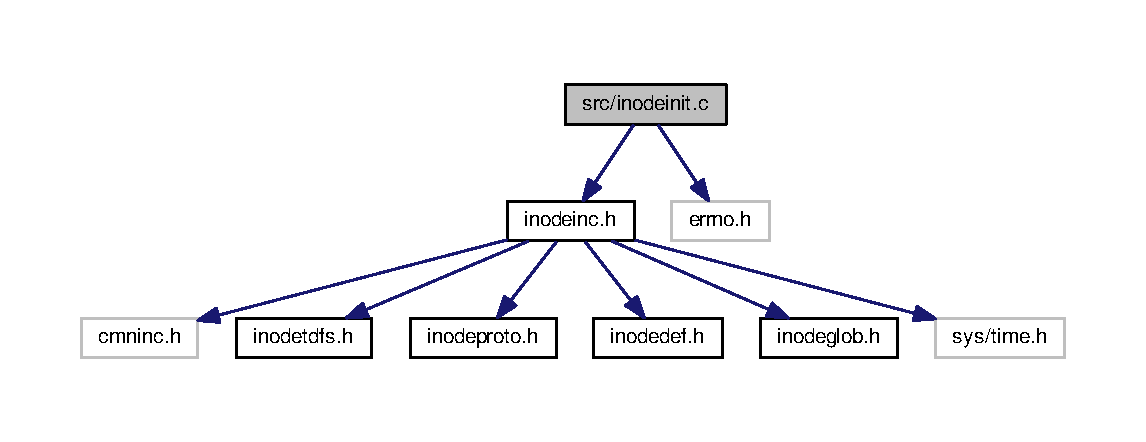
\includegraphics[width=350pt]{inodeinit_8c__incl}
\end{center}
\end{figure}
\subsection*{Functions}
\begin{DoxyCompactItemize}
\item 
V\+O\+I\+D \hyperlink{inodeinit_8c_a8baf7fbbf3bd018d0474920abbe85b5c}{Inode\+Init} (C\+H\+A\+R $\ast$p\+Dev)
\item 
I\+N\+T4 \hyperlink{inodeinit_8c_a29e6d4d69a3bddfbaf2d36c9702b35a7}{Inode\+Init\+Read\+Super\+Block} ()
\item 
V\+O\+I\+D \hyperlink{inodeinit_8c_a2276ef70d6539482065832e9f96b7328}{Inode\+Init\+Exit} ()
\end{DoxyCompactItemize}


\subsection{Function Documentation}
\hypertarget{inodeinit_8c_a8baf7fbbf3bd018d0474920abbe85b5c}{\index{inodeinit.\+c@{inodeinit.\+c}!Inode\+Init@{Inode\+Init}}
\index{Inode\+Init@{Inode\+Init}!inodeinit.\+c@{inodeinit.\+c}}
\subsubsection[{Inode\+Init}]{\setlength{\rightskip}{0pt plus 5cm}V\+O\+I\+D Inode\+Init (
\begin{DoxyParamCaption}
\item[{C\+H\+A\+R $\ast$}]{p\+Dev}
\end{DoxyParamCaption}
)}}\label{inodeinit_8c_a8baf7fbbf3bd018d0474920abbe85b5c}


 Function Name \+: Inode\+Init

Description \+: This Function is used to Initialize the inode module.

Input \+: p\+Dev -\/ name of the device to open

Output \+: None

Returns \+: None 

Here is the call graph for this function\+:\nopagebreak
\begin{figure}[H]
\begin{center}
\leavevmode
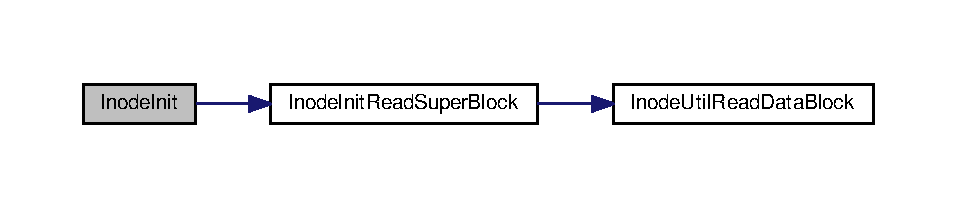
\includegraphics[width=350pt]{inodeinit_8c_a8baf7fbbf3bd018d0474920abbe85b5c_cgraph}
\end{center}
\end{figure}


\hypertarget{inodeinit_8c_a2276ef70d6539482065832e9f96b7328}{\index{inodeinit.\+c@{inodeinit.\+c}!Inode\+Init\+Exit@{Inode\+Init\+Exit}}
\index{Inode\+Init\+Exit@{Inode\+Init\+Exit}!inodeinit.\+c@{inodeinit.\+c}}
\subsubsection[{Inode\+Init\+Exit}]{\setlength{\rightskip}{0pt plus 5cm}V\+O\+I\+D Inode\+Init\+Exit (
\begin{DoxyParamCaption}
{}
\end{DoxyParamCaption}
)}}\label{inodeinit_8c_a2276ef70d6539482065832e9f96b7328}


 Function Name \+: Inode\+Init\+Exit

Description \+: This Function is used to destroy the initialized parameters before exiting the program.

Input \+: None

Output \+: None

Returns \+: None \hypertarget{inodeinit_8c_a29e6d4d69a3bddfbaf2d36c9702b35a7}{\index{inodeinit.\+c@{inodeinit.\+c}!Inode\+Init\+Read\+Super\+Block@{Inode\+Init\+Read\+Super\+Block}}
\index{Inode\+Init\+Read\+Super\+Block@{Inode\+Init\+Read\+Super\+Block}!inodeinit.\+c@{inodeinit.\+c}}
\subsubsection[{Inode\+Init\+Read\+Super\+Block}]{\setlength{\rightskip}{0pt plus 5cm}I\+N\+T4 Inode\+Init\+Read\+Super\+Block (
\begin{DoxyParamCaption}
{}
\end{DoxyParamCaption}
)}}\label{inodeinit_8c_a29e6d4d69a3bddfbaf2d36c9702b35a7}


 Function Name \+: Inode\+Init\+Read\+Super\+Block

Description \+: This Function is used to read the super block.

Input \+: None

Output \+: None

Returns \+: None 

Here is the call graph for this function\+:\nopagebreak
\begin{figure}[H]
\begin{center}
\leavevmode
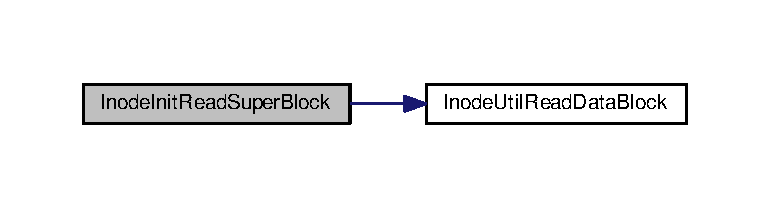
\includegraphics[width=350pt]{inodeinit_8c_a29e6d4d69a3bddfbaf2d36c9702b35a7_cgraph}
\end{center}
\end{figure}



\hypertarget{inodemain_8c}{\section{src/inodemain.c File Reference}
\label{inodemain_8c}\index{src/inodemain.\+c@{src/inodemain.\+c}}
}
{\ttfamily \#include \char`\"{}inodeinc.\+h\char`\"{}}\\*
{\ttfamily \#include \char`\"{}inodecli.\+h\char`\"{}}\\*
Include dependency graph for inodemain.\+c\+:\nopagebreak
\begin{figure}[H]
\begin{center}
\leavevmode
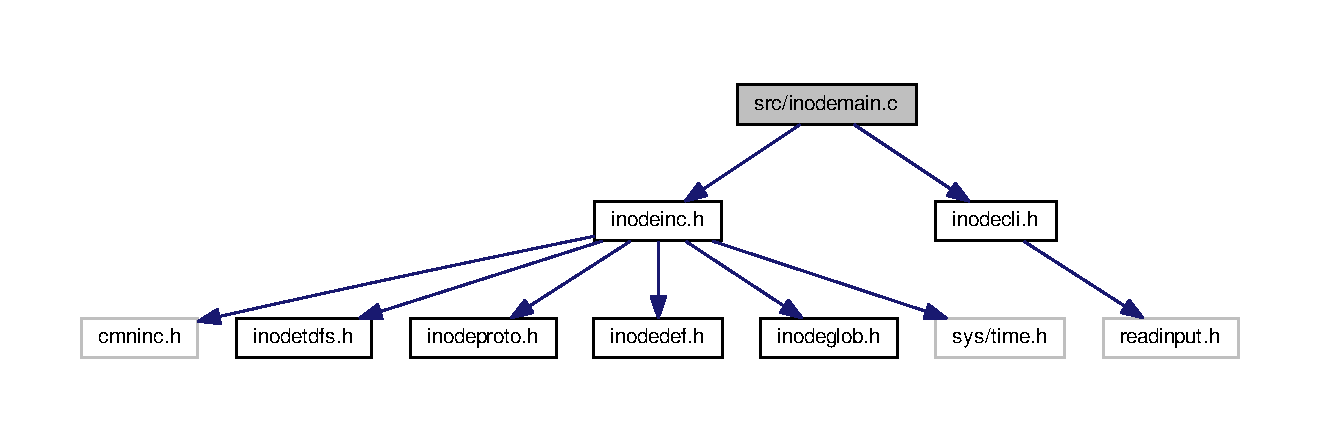
\includegraphics[width=350pt]{inodemain_8c__incl}
\end{center}
\end{figure}
\subsection*{Functions}
\begin{DoxyCompactItemize}
\item 
V\+O\+I\+D \hyperlink{inodemain_8c_a01fd3059d6c6fa9b86faae2a52379fef}{main} (I\+N\+T4 argc, C\+H\+A\+R $\ast$$\ast$argv)
\end{DoxyCompactItemize}


\subsection{Function Documentation}
\hypertarget{inodemain_8c_a01fd3059d6c6fa9b86faae2a52379fef}{\index{inodemain.\+c@{inodemain.\+c}!main@{main}}
\index{main@{main}!inodemain.\+c@{inodemain.\+c}}
\subsubsection[{main}]{\setlength{\rightskip}{0pt plus 5cm}V\+O\+I\+D main (
\begin{DoxyParamCaption}
\item[{I\+N\+T4}]{argc, }
\item[{C\+H\+A\+R $\ast$$\ast$}]{argv}
\end{DoxyParamCaption}
)}}\label{inodemain_8c_a01fd3059d6c6fa9b86faae2a52379fef}


 Function Name \+: main

Description \+: This is the \hyperlink{inodemain_8c_a01fd3059d6c6fa9b86faae2a52379fef}{main()} function for the inode program.

Input \+: argc -\/ total no. of command line arguments argv -\/ command line arguments

Output \+: None

Returns \+: None 

Here is the call graph for this function\+:\nopagebreak
\begin{figure}[H]
\begin{center}
\leavevmode
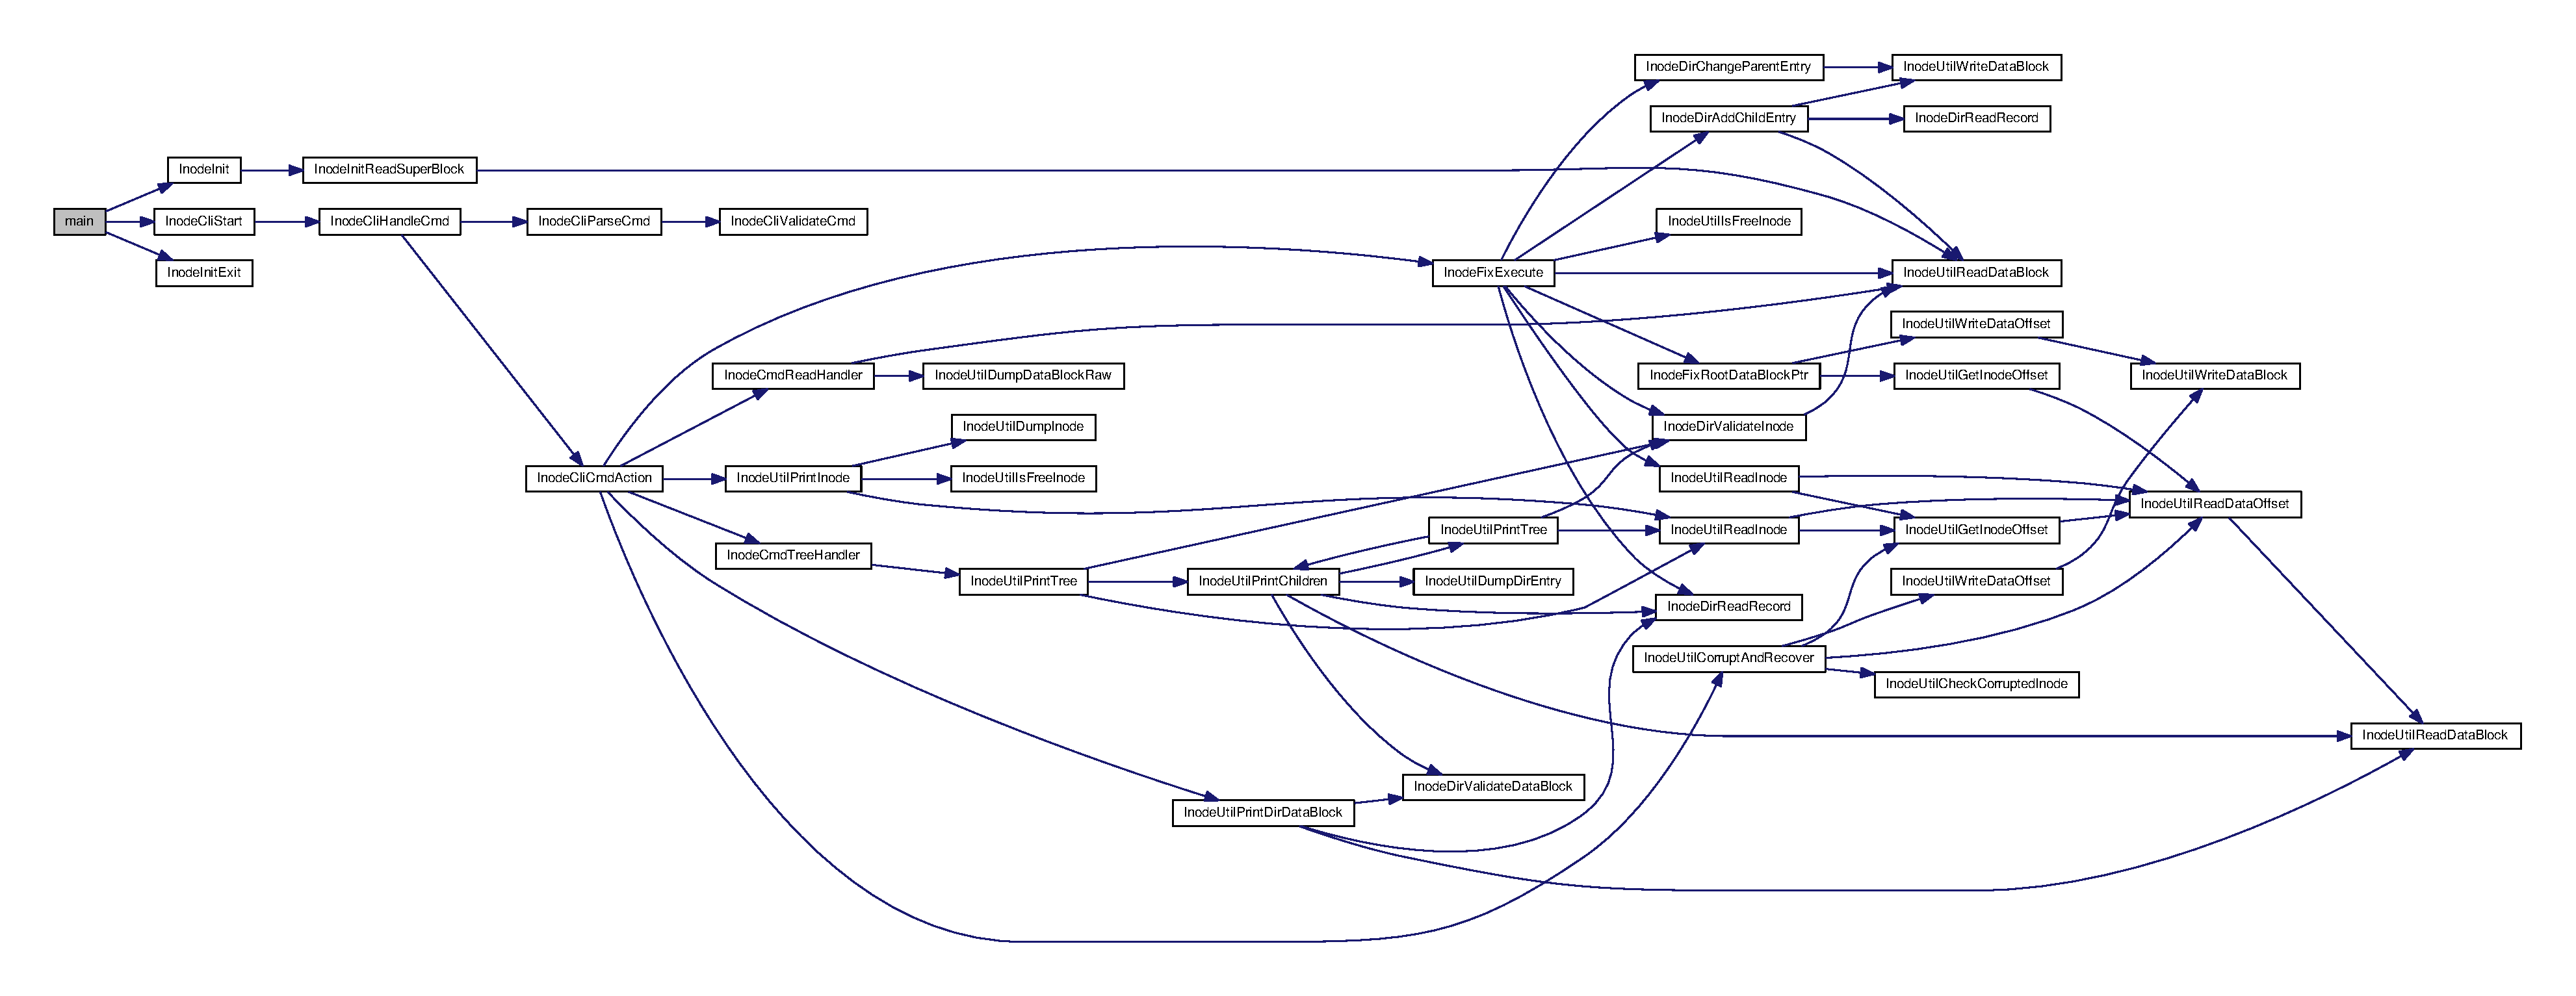
\includegraphics[width=350pt]{inodemain_8c_a01fd3059d6c6fa9b86faae2a52379fef_cgraph}
\end{center}
\end{figure}



\hypertarget{inodeutil_8c}{\section{src/inodeutil.c File Reference}
\label{inodeutil_8c}\index{src/inodeutil.\+c@{src/inodeutil.\+c}}
}
{\ttfamily \#include \char`\"{}inodeinc.\+h\char`\"{}}\\*
Include dependency graph for inodeutil.\+c\+:\nopagebreak
\begin{figure}[H]
\begin{center}
\leavevmode
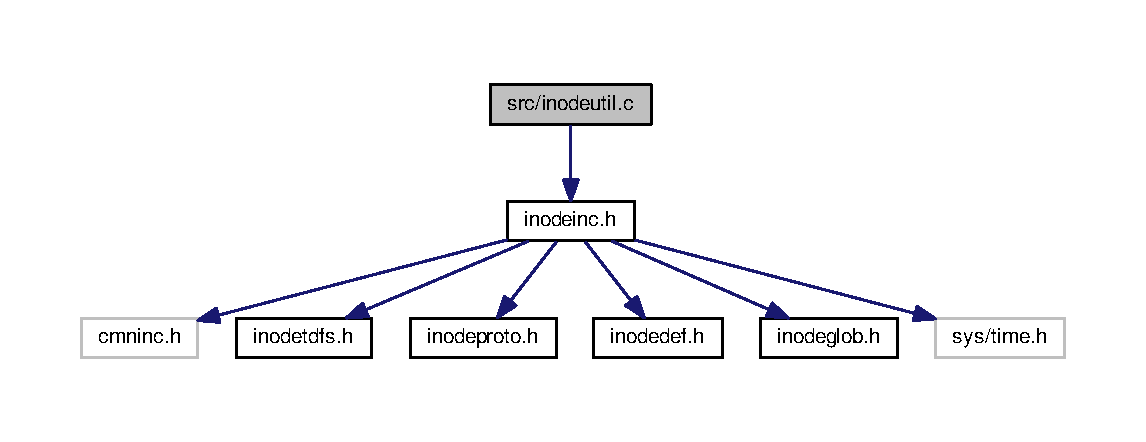
\includegraphics[width=350pt]{inodeutil_8c__incl}
\end{center}
\end{figure}
\subsection*{Functions}
\begin{DoxyCompactItemize}
\item 
I\+N\+T4 \hyperlink{inodeutil_8c_a45685e5c715aa741d487eae77c1083ae}{Inode\+Util\+Print\+Inode} (U\+I\+N\+T4 u4\+Inode\+No)
\item 
I\+N\+T4 \hyperlink{inodeutil_8c_af3bd13d59e79a9c574862e0a42ac1ac2}{Inode\+Util\+Print\+Tree} (U\+I\+N\+T4 u4\+Inode\+No, U\+I\+N\+T4 u4\+Level)
\item 
I\+N\+T4 \hyperlink{inodeutil_8c_a6474c5fd62b8ca4f7745428690849175}{Inode\+Util\+Print\+Children} (U\+I\+N\+T4 u4\+Block\+No, U\+I\+N\+T4 u4\+Level)
\item 
I\+N\+T4 \hyperlink{inodeutil_8c_a0bb419219a634fdfbb0e32df8fd4f937}{Inode\+Util\+Print\+Dir\+Data\+Block} (U\+I\+N\+T4 u4\+Block\+No)
\item 
I\+N\+T4 \hyperlink{inodeutil_8c_a13b5c799edb137a494ad497145f59a56}{Inode\+Util\+Read\+Data\+Block} (U\+I\+N\+T4 u4\+Block\+No, U\+I\+N\+T2 u2\+Start\+Pos, V\+O\+I\+D $\ast$p\+Buffer, U\+I\+N\+T4 u4\+Size)
\item 
I\+N\+T4 \hyperlink{inodeutil_8c_a3add91b54cfb3e27f802ac8ab1b9ceb4}{Inode\+Util\+Read\+Data\+Offset} (U\+I\+N\+T8 u8\+Offset, V\+O\+I\+D $\ast$p\+Buffer, U\+I\+N\+T4 u4\+Size)
\item 
I\+N\+T4 \hyperlink{inodeutil_8c_af4e29989b8cc9424603a4825af3491a0}{Inode\+Util\+Write\+Data\+Block} (U\+I\+N\+T4 u4\+Block\+No, U\+I\+N\+T2 u2\+Start\+Pos, V\+O\+I\+D $\ast$p\+Buffer, U\+I\+N\+T4 u4\+Size)
\item 
I\+N\+T4 \hyperlink{inodeutil_8c_a9671fcb9023997872ade29c0241b0cab}{Inode\+Util\+Write\+Data\+Offset} (U\+I\+N\+T8 u8\+Offset, V\+O\+I\+D $\ast$p\+Buffer, U\+I\+N\+T4 u4\+Size)
\item 
I\+N\+T4 \hyperlink{inodeutil_8c_a8c820c9998f3a81b0b7efb2336e3ebc4}{Inode\+Util\+Read\+Inode} (U\+I\+N\+T4 u4\+Inode\+No, struct ext3\+\_\+inode $\ast$p\+New\+Inode)
\item 
V\+O\+I\+D \hyperlink{inodeutil_8c_af56b9ef4fbba04cbcdc61dfcda95c33b}{Inode\+Util\+Dump\+Dir\+Entry} (struct ext3\+\_\+dir\+\_\+entry\+\_\+2 $\ast$p\+Dir\+Entry, \hyperlink{inodetdfs_8h_a408cefd7ee29ff67ed7fefab9393affa}{t\+File\+Filter} Filter, U\+I\+N\+T4 u4\+Level)
\item 
V\+O\+I\+D \hyperlink{inodeutil_8c_a02fc70420f966503493dcee4f275951c}{Inode\+Util\+Dump\+Inode} (struct ext3\+\_\+inode $\ast$p\+Inode)
\item 
V\+O\+I\+D \hyperlink{inodeutil_8c_a91e76cac49f4444a82a74a2fa004011d}{Inode\+Util\+Dump\+Data\+Block\+Raw} (C\+H\+A\+R $\ast$p\+Buffer)
\item 
I\+N\+T4 \hyperlink{inodeutil_8c_a5aa634acb8fba879d55a5de096d3997c}{Inode\+Util\+Get\+Inode\+Offset} (U\+I\+N\+T4 u4\+Inode\+No, U\+I\+N\+T8 $\ast$pu8\+Offset)
\item 
I\+N\+T4 \hyperlink{inodeutil_8c_a091aeb9997faf9dae00a698c470439e9}{Inode\+Util\+Check\+Corrupted\+Inode} (U\+I\+N\+T4 u4\+Inode\+No)
\item 
I\+N\+T4 \hyperlink{inodeutil_8c_ae4aa54c12d8e18c272feab11068a1cfb}{Inode\+Util\+Corrupt\+And\+Recover} (U\+I\+N\+T4 u4\+Inode\+No, U\+I\+N\+T4 u4\+Cmd)
\item 
I\+N\+T1 \hyperlink{inodeutil_8c_a63b7552b4e10719ea82758cb689850a8}{Inode\+Util\+Is\+Free\+Inode} (struct ext3\+\_\+inode $\ast$p\+Inode)
\end{DoxyCompactItemize}


\subsection{Function Documentation}
\hypertarget{inodeutil_8c_a091aeb9997faf9dae00a698c470439e9}{\index{inodeutil.\+c@{inodeutil.\+c}!Inode\+Util\+Check\+Corrupted\+Inode@{Inode\+Util\+Check\+Corrupted\+Inode}}
\index{Inode\+Util\+Check\+Corrupted\+Inode@{Inode\+Util\+Check\+Corrupted\+Inode}!inodeutil.\+c@{inodeutil.\+c}}
\subsubsection[{Inode\+Util\+Check\+Corrupted\+Inode}]{\setlength{\rightskip}{0pt plus 5cm}I\+N\+T4 Inode\+Util\+Check\+Corrupted\+Inode (
\begin{DoxyParamCaption}
\item[{U\+I\+N\+T4}]{u4\+Inode\+No}
\end{DoxyParamCaption}
)}}\label{inodeutil_8c_a091aeb9997faf9dae00a698c470439e9}


 Function Name \+: Inode\+Util\+Check\+Corrupted\+Inode

Author \+: Anusha Seshadri

Description \+: This Function is used during manual corruption to check whether the inode is already corrupted manually or not.

Input \+: u4\+Inode\+No -\/ Inode number

Output \+: None

Returns \+: array index in the corrupted array, if the inode is corrupted I\+N\+O\+D\+E\+\_\+\+F\+A\+I\+L\+U\+R\+E if it is not corrupted already \hypertarget{inodeutil_8c_ae4aa54c12d8e18c272feab11068a1cfb}{\index{inodeutil.\+c@{inodeutil.\+c}!Inode\+Util\+Corrupt\+And\+Recover@{Inode\+Util\+Corrupt\+And\+Recover}}
\index{Inode\+Util\+Corrupt\+And\+Recover@{Inode\+Util\+Corrupt\+And\+Recover}!inodeutil.\+c@{inodeutil.\+c}}
\subsubsection[{Inode\+Util\+Corrupt\+And\+Recover}]{\setlength{\rightskip}{0pt plus 5cm}I\+N\+T4 Inode\+Util\+Corrupt\+And\+Recover (
\begin{DoxyParamCaption}
\item[{U\+I\+N\+T4}]{u4\+Inode\+No, }
\item[{U\+I\+N\+T4}]{u4\+Cmd}
\end{DoxyParamCaption}
)}}\label{inodeutil_8c_ae4aa54c12d8e18c272feab11068a1cfb}


 Function Name \+: Inode\+Util\+Corrupt\+And\+Recover

Author \+: Anusha Seshadri

Description \+: This Function is used to manually corrupt and fix an inode.

Input \+: u4\+Inode\+No -\/ Inode to corrupt/fix u4\+Cmd -\/ I\+N\+O\+D\+E\+\_\+\+C\+O\+R\+R\+U\+P\+T to corrupt I\+N\+O\+D\+E\+\_\+\+F\+I\+X to fix Output \+: None

Returns \+: I\+N\+O\+D\+E\+\_\+\+S\+U\+C\+C\+E\+S\+S I\+N\+O\+D\+E\+\_\+\+F\+A\+I\+L\+U\+R\+E 

Here is the call graph for this function\+:\nopagebreak
\begin{figure}[H]
\begin{center}
\leavevmode
\includegraphics[width=350pt]{inodeutil_8c_ae4aa54c12d8e18c272feab11068a1cfb_cgraph}
\end{center}
\end{figure}


\hypertarget{inodeutil_8c_a91e76cac49f4444a82a74a2fa004011d}{\index{inodeutil.\+c@{inodeutil.\+c}!Inode\+Util\+Dump\+Data\+Block\+Raw@{Inode\+Util\+Dump\+Data\+Block\+Raw}}
\index{Inode\+Util\+Dump\+Data\+Block\+Raw@{Inode\+Util\+Dump\+Data\+Block\+Raw}!inodeutil.\+c@{inodeutil.\+c}}
\subsubsection[{Inode\+Util\+Dump\+Data\+Block\+Raw}]{\setlength{\rightskip}{0pt plus 5cm}V\+O\+I\+D Inode\+Util\+Dump\+Data\+Block\+Raw (
\begin{DoxyParamCaption}
\item[{C\+H\+A\+R $\ast$}]{p\+Buffer}
\end{DoxyParamCaption}
)}}\label{inodeutil_8c_a91e76cac49f4444a82a74a2fa004011d}


 Function Name \+: Inode\+Util\+Dump\+Data\+Block\+Raw

Author \+: Naveen Raj Selvaraj

Description \+: This Function is used to print the content of a block in H\+E\+X

Input \+: p\+Buffer -\/ buffer containing the data block contents

Output \+: None

Returns \+: None \hypertarget{inodeutil_8c_af56b9ef4fbba04cbcdc61dfcda95c33b}{\index{inodeutil.\+c@{inodeutil.\+c}!Inode\+Util\+Dump\+Dir\+Entry@{Inode\+Util\+Dump\+Dir\+Entry}}
\index{Inode\+Util\+Dump\+Dir\+Entry@{Inode\+Util\+Dump\+Dir\+Entry}!inodeutil.\+c@{inodeutil.\+c}}
\subsubsection[{Inode\+Util\+Dump\+Dir\+Entry}]{\setlength{\rightskip}{0pt plus 5cm}V\+O\+I\+D Inode\+Util\+Dump\+Dir\+Entry (
\begin{DoxyParamCaption}
\item[{struct ext3\+\_\+dir\+\_\+entry\+\_\+2 $\ast$}]{p\+Dir\+Entry, }
\item[{{\bf t\+File\+Filter}}]{Filter, }
\item[{U\+I\+N\+T4}]{u4\+Level}
\end{DoxyParamCaption}
)}}\label{inodeutil_8c_af56b9ef4fbba04cbcdc61dfcda95c33b}


 Function Name \+: Inode\+Util\+Dump\+Dir\+Entry

Author \+: Naveen Raj Selvaraj

Description \+: This Function is used to print a directory entry.

Input \+: p\+Dir\+Entry -\/ pointer to the directory entry to print Filter -\/ F\+I\+L\+E\+\_\+\+T\+Y\+P\+E\+\_\+\+D\+I\+R\+S -\/ print only directories F\+I\+L\+E\+\_\+\+T\+Y\+P\+E\+\_\+\+F\+I\+L\+E\+S -\/ print directories and files F\+I\+L\+E\+\_\+\+T\+Y\+P\+E\+\_\+\+A\+L\+L -\/ print everything including . and .. entries u4\+Level -\/ depth of this entry in the tree (used to format the output) Output \+: None

Returns \+: None \hypertarget{inodeutil_8c_a02fc70420f966503493dcee4f275951c}{\index{inodeutil.\+c@{inodeutil.\+c}!Inode\+Util\+Dump\+Inode@{Inode\+Util\+Dump\+Inode}}
\index{Inode\+Util\+Dump\+Inode@{Inode\+Util\+Dump\+Inode}!inodeutil.\+c@{inodeutil.\+c}}
\subsubsection[{Inode\+Util\+Dump\+Inode}]{\setlength{\rightskip}{0pt plus 5cm}V\+O\+I\+D Inode\+Util\+Dump\+Inode (
\begin{DoxyParamCaption}
\item[{struct ext3\+\_\+inode $\ast$}]{p\+Inode}
\end{DoxyParamCaption}
)}}\label{inodeutil_8c_a02fc70420f966503493dcee4f275951c}


 Function Name \+: Inode\+Util\+Dump\+Inode

Author \+: Naveen Raj Selvaraj

Description \+: This Function is used to print the ext3\+\_\+inode structure

Input \+: p\+Inode -\/ pointer to the inode structure

Output \+: None

Returns \+: None \hypertarget{inodeutil_8c_a5aa634acb8fba879d55a5de096d3997c}{\index{inodeutil.\+c@{inodeutil.\+c}!Inode\+Util\+Get\+Inode\+Offset@{Inode\+Util\+Get\+Inode\+Offset}}
\index{Inode\+Util\+Get\+Inode\+Offset@{Inode\+Util\+Get\+Inode\+Offset}!inodeutil.\+c@{inodeutil.\+c}}
\subsubsection[{Inode\+Util\+Get\+Inode\+Offset}]{\setlength{\rightskip}{0pt plus 5cm}I\+N\+T4 Inode\+Util\+Get\+Inode\+Offset (
\begin{DoxyParamCaption}
\item[{U\+I\+N\+T4}]{u4\+Inode\+No, }
\item[{U\+I\+N\+T8 $\ast$}]{pu8\+Offset}
\end{DoxyParamCaption}
)}}\label{inodeutil_8c_a5aa634acb8fba879d55a5de096d3997c}


 Function Name \+: Inode\+Util\+Get\+Inode\+Offset

Author \+: Naveen Raj Selvaraj

Description \+: This Function is used to convert the given inode number into byte offset

Input \+: u4\+Inode\+No -\/ Inode number

Output \+: pu8\+Offset -\/ byte offset

Returns \+: I\+N\+O\+D\+E\+\_\+\+S\+U\+C\+C\+E\+S\+S, if the byte offset can be calculated I\+N\+O\+D\+E\+\_\+\+F\+A\+I\+L\+U\+R\+E otherwise 

Here is the call graph for this function\+:\nopagebreak
\begin{figure}[H]
\begin{center}
\leavevmode
\includegraphics[width=350pt]{inodeutil_8c_a5aa634acb8fba879d55a5de096d3997c_cgraph}
\end{center}
\end{figure}


\hypertarget{inodeutil_8c_a63b7552b4e10719ea82758cb689850a8}{\index{inodeutil.\+c@{inodeutil.\+c}!Inode\+Util\+Is\+Free\+Inode@{Inode\+Util\+Is\+Free\+Inode}}
\index{Inode\+Util\+Is\+Free\+Inode@{Inode\+Util\+Is\+Free\+Inode}!inodeutil.\+c@{inodeutil.\+c}}
\subsubsection[{Inode\+Util\+Is\+Free\+Inode}]{\setlength{\rightskip}{0pt plus 5cm}I\+N\+T1 Inode\+Util\+Is\+Free\+Inode (
\begin{DoxyParamCaption}
\item[{struct ext3\+\_\+inode $\ast$}]{p\+Inode}
\end{DoxyParamCaption}
)}}\label{inodeutil_8c_a63b7552b4e10719ea82758cb689850a8}


 Function Name \+: Inode\+Util\+Is\+Free\+Inode

Author \+: Naveen Raj Selvaraj

Description \+: This Function is used to check if an inode is all zero

Input \+: p\+Inode -\/ pointer to the inode structure

Output \+: None

Returns \+: T\+R\+U\+E, if the inode is free F\+A\+L\+S\+E otherwise \hypertarget{inodeutil_8c_a6474c5fd62b8ca4f7745428690849175}{\index{inodeutil.\+c@{inodeutil.\+c}!Inode\+Util\+Print\+Children@{Inode\+Util\+Print\+Children}}
\index{Inode\+Util\+Print\+Children@{Inode\+Util\+Print\+Children}!inodeutil.\+c@{inodeutil.\+c}}
\subsubsection[{Inode\+Util\+Print\+Children}]{\setlength{\rightskip}{0pt plus 5cm}I\+N\+T4 Inode\+Util\+Print\+Children (
\begin{DoxyParamCaption}
\item[{U\+I\+N\+T4}]{u4\+Block\+No, }
\item[{U\+I\+N\+T4}]{u4\+Level}
\end{DoxyParamCaption}
)}}\label{inodeutil_8c_a6474c5fd62b8ca4f7745428690849175}


 Function Name \+: Inode\+Util\+Print\+Children

Author \+: Naveen Raj Selvaraj

Description \+: This Function is used to print the children of a directory inode as a part of printing the tree. If the child is a directory inode, then it calls the Inode\+Util\+Print\+Tree function to print the subtree of that child.

Input \+: u4\+Block\+No -\/ Data block of a directory inode u4\+Level -\/ number inidicating the depth of the file system object in the tree.(used to format the output)

Output \+: None

Returns \+: I\+N\+O\+D\+E\+\_\+\+S\+U\+C\+C\+E\+S\+S, when successfully printed I\+N\+O\+D\+E\+\_\+\+F\+A\+I\+L\+U\+R\+E otherwise 

Here is the call graph for this function\+:\nopagebreak
\begin{figure}[H]
\begin{center}
\leavevmode
\includegraphics[width=350pt]{inodeutil_8c_a6474c5fd62b8ca4f7745428690849175_cgraph}
\end{center}
\end{figure}


\hypertarget{inodeutil_8c_a0bb419219a634fdfbb0e32df8fd4f937}{\index{inodeutil.\+c@{inodeutil.\+c}!Inode\+Util\+Print\+Dir\+Data\+Block@{Inode\+Util\+Print\+Dir\+Data\+Block}}
\index{Inode\+Util\+Print\+Dir\+Data\+Block@{Inode\+Util\+Print\+Dir\+Data\+Block}!inodeutil.\+c@{inodeutil.\+c}}
\subsubsection[{Inode\+Util\+Print\+Dir\+Data\+Block}]{\setlength{\rightskip}{0pt plus 5cm}I\+N\+T4 Inode\+Util\+Print\+Dir\+Data\+Block (
\begin{DoxyParamCaption}
\item[{U\+I\+N\+T4}]{u4\+Block\+No}
\end{DoxyParamCaption}
)}}\label{inodeutil_8c_a0bb419219a634fdfbb0e32df8fd4f937}


 Function Name \+: Inode\+Util\+Print\+Dir\+Data\+Block

Author \+: Naveen Raj Selvaraj

Description \+: This Function is used to print the directory entries present in a directory data block

Input \+: u4\+Block\+No -\/ directory data block number

Output \+: None

Returns \+: I\+N\+O\+D\+E\+\_\+\+S\+U\+C\+C\+E\+S\+S, when successfully printed I\+N\+O\+D\+E\+\_\+\+F\+A\+I\+L\+U\+R\+E otherwise 

Here is the call graph for this function\+:\nopagebreak
\begin{figure}[H]
\begin{center}
\leavevmode
\includegraphics[width=350pt]{inodeutil_8c_a0bb419219a634fdfbb0e32df8fd4f937_cgraph}
\end{center}
\end{figure}


\hypertarget{inodeutil_8c_a45685e5c715aa741d487eae77c1083ae}{\index{inodeutil.\+c@{inodeutil.\+c}!Inode\+Util\+Print\+Inode@{Inode\+Util\+Print\+Inode}}
\index{Inode\+Util\+Print\+Inode@{Inode\+Util\+Print\+Inode}!inodeutil.\+c@{inodeutil.\+c}}
\subsubsection[{Inode\+Util\+Print\+Inode}]{\setlength{\rightskip}{0pt plus 5cm}I\+N\+T4 Inode\+Util\+Print\+Inode (
\begin{DoxyParamCaption}
\item[{U\+I\+N\+T4}]{u4\+Inode\+No}
\end{DoxyParamCaption}
)}}\label{inodeutil_8c_a45685e5c715aa741d487eae77c1083ae}


 Function Name \+: Inode\+Util\+Print\+Inode

Author \+: Naveen Raj Selvaraj

Description \+: This Function is used to print the contents of an inode

Input \+: u4\+Inode\+No -\/ Inode number

Output \+: None

Returns \+: I\+N\+O\+D\+E\+\_\+\+S\+U\+C\+C\+E\+S\+S, when successfully printed I\+N\+O\+D\+E\+\_\+\+F\+A\+I\+L\+U\+R\+E otherwise 

Here is the call graph for this function\+:\nopagebreak
\begin{figure}[H]
\begin{center}
\leavevmode
\includegraphics[width=350pt]{inodeutil_8c_a45685e5c715aa741d487eae77c1083ae_cgraph}
\end{center}
\end{figure}


\hypertarget{inodeutil_8c_af3bd13d59e79a9c574862e0a42ac1ac2}{\index{inodeutil.\+c@{inodeutil.\+c}!Inode\+Util\+Print\+Tree@{Inode\+Util\+Print\+Tree}}
\index{Inode\+Util\+Print\+Tree@{Inode\+Util\+Print\+Tree}!inodeutil.\+c@{inodeutil.\+c}}
\subsubsection[{Inode\+Util\+Print\+Tree}]{\setlength{\rightskip}{0pt plus 5cm}I\+N\+T4 Inode\+Util\+Print\+Tree (
\begin{DoxyParamCaption}
\item[{U\+I\+N\+T4}]{u4\+Inode\+No, }
\item[{U\+I\+N\+T4}]{u4\+Level}
\end{DoxyParamCaption}
)}}\label{inodeutil_8c_af3bd13d59e79a9c574862e0a42ac1ac2}


 Function Name \+: Inode\+Util\+Print\+Tree

Author \+: Naveen Raj Selvaraj

Description \+: This Function is used to print the tree/subtree of the file system objects starting at a specified directory inode in depth first order.

Input \+: u4\+Inode\+No -\/ Inode number u4\+Level -\/ number inidicating the depth of the file system object in the tree (this is used to format the output. e.\+g\+: root inode for the tree should be called with u4\+Level = 1) Output \+: None

Returns \+: I\+N\+O\+D\+E\+\_\+\+S\+U\+C\+C\+E\+S\+S, when successfully printed I\+N\+O\+D\+E\+\_\+\+F\+A\+I\+L\+U\+R\+E otherwise 

Here is the call graph for this function\+:\nopagebreak
\begin{figure}[H]
\begin{center}
\leavevmode
\includegraphics[width=350pt]{inodeutil_8c_af3bd13d59e79a9c574862e0a42ac1ac2_cgraph}
\end{center}
\end{figure}


\hypertarget{inodeutil_8c_a13b5c799edb137a494ad497145f59a56}{\index{inodeutil.\+c@{inodeutil.\+c}!Inode\+Util\+Read\+Data\+Block@{Inode\+Util\+Read\+Data\+Block}}
\index{Inode\+Util\+Read\+Data\+Block@{Inode\+Util\+Read\+Data\+Block}!inodeutil.\+c@{inodeutil.\+c}}
\subsubsection[{Inode\+Util\+Read\+Data\+Block}]{\setlength{\rightskip}{0pt plus 5cm}I\+N\+T4 Inode\+Util\+Read\+Data\+Block (
\begin{DoxyParamCaption}
\item[{U\+I\+N\+T4}]{u4\+Block\+No, }
\item[{U\+I\+N\+T2}]{u2\+Start\+Pos, }
\item[{V\+O\+I\+D $\ast$}]{p\+Buffer, }
\item[{U\+I\+N\+T4}]{u4\+Size}
\end{DoxyParamCaption}
)}}\label{inodeutil_8c_a13b5c799edb137a494ad497145f59a56}


 Function Name \+: Inode\+Util\+Read\+Data\+Block

Author \+: Naveen Raj Selvaraj

Description \+: This Function is used to read a file system block

Input \+: u4\+Block\+No -\/ Block number to read u4\+Size -\/ size of data to read in bytes

Output \+: p\+Buffer -\/ Buffer containg the contents of the block

Returns \+: I\+N\+O\+D\+E\+\_\+\+S\+U\+C\+C\+E\+S\+S, if the read succeeds I\+N\+O\+D\+E\+\_\+\+F\+A\+I\+L\+U\+R\+E otherwise \hypertarget{inodeutil_8c_a3add91b54cfb3e27f802ac8ab1b9ceb4}{\index{inodeutil.\+c@{inodeutil.\+c}!Inode\+Util\+Read\+Data\+Offset@{Inode\+Util\+Read\+Data\+Offset}}
\index{Inode\+Util\+Read\+Data\+Offset@{Inode\+Util\+Read\+Data\+Offset}!inodeutil.\+c@{inodeutil.\+c}}
\subsubsection[{Inode\+Util\+Read\+Data\+Offset}]{\setlength{\rightskip}{0pt plus 5cm}I\+N\+T4 Inode\+Util\+Read\+Data\+Offset (
\begin{DoxyParamCaption}
\item[{U\+I\+N\+T8}]{u8\+Offset, }
\item[{V\+O\+I\+D $\ast$}]{p\+Buffer, }
\item[{U\+I\+N\+T4}]{u4\+Size}
\end{DoxyParamCaption}
)}}\label{inodeutil_8c_a3add91b54cfb3e27f802ac8ab1b9ceb4}


 Function Name \+: Inode\+Util\+Read\+Data\+Offset

Author \+: Naveen Raj Selvaraj

Description \+: This Function is used to read data from any location

Input \+: u8\+Offset -\/ Byte offset to read u4\+Size -\/ size of data to read in bytes

Output \+: p\+Buffer -\/ Buffer containg the contents of the block

Returns \+: I\+N\+O\+D\+E\+\_\+\+S\+U\+C\+C\+E\+S\+S, if the read succeeds I\+N\+O\+D\+E\+\_\+\+F\+A\+I\+L\+U\+R\+E otherwise 

Here is the call graph for this function\+:\nopagebreak
\begin{figure}[H]
\begin{center}
\leavevmode
\includegraphics[width=350pt]{inodeutil_8c_a3add91b54cfb3e27f802ac8ab1b9ceb4_cgraph}
\end{center}
\end{figure}


\hypertarget{inodeutil_8c_a8c820c9998f3a81b0b7efb2336e3ebc4}{\index{inodeutil.\+c@{inodeutil.\+c}!Inode\+Util\+Read\+Inode@{Inode\+Util\+Read\+Inode}}
\index{Inode\+Util\+Read\+Inode@{Inode\+Util\+Read\+Inode}!inodeutil.\+c@{inodeutil.\+c}}
\subsubsection[{Inode\+Util\+Read\+Inode}]{\setlength{\rightskip}{0pt plus 5cm}I\+N\+T4 Inode\+Util\+Read\+Inode (
\begin{DoxyParamCaption}
\item[{U\+I\+N\+T4}]{u4\+Inode\+No, }
\item[{struct ext3\+\_\+inode $\ast$}]{p\+New\+Inode}
\end{DoxyParamCaption}
)}}\label{inodeutil_8c_a8c820c9998f3a81b0b7efb2336e3ebc4}


 Function Name \+: Inode\+Util\+Read\+Inode

Author \+: Naveen Raj Selvaraj

Description \+: This Function is used to read an inode

Input \+: u4\+Inode\+No -\/ Inode number to read

Output \+: p\+New\+Inode -\/ pointer to the structure containing the inode contents

Returns \+: I\+N\+O\+D\+E\+\_\+\+S\+U\+C\+C\+E\+S\+S, on successful read I\+N\+O\+D\+E\+\_\+\+F\+A\+I\+L\+U\+R\+E otherwise 

Here is the call graph for this function\+:\nopagebreak
\begin{figure}[H]
\begin{center}
\leavevmode
\includegraphics[width=350pt]{inodeutil_8c_a8c820c9998f3a81b0b7efb2336e3ebc4_cgraph}
\end{center}
\end{figure}


\hypertarget{inodeutil_8c_af4e29989b8cc9424603a4825af3491a0}{\index{inodeutil.\+c@{inodeutil.\+c}!Inode\+Util\+Write\+Data\+Block@{Inode\+Util\+Write\+Data\+Block}}
\index{Inode\+Util\+Write\+Data\+Block@{Inode\+Util\+Write\+Data\+Block}!inodeutil.\+c@{inodeutil.\+c}}
\subsubsection[{Inode\+Util\+Write\+Data\+Block}]{\setlength{\rightskip}{0pt plus 5cm}I\+N\+T4 Inode\+Util\+Write\+Data\+Block (
\begin{DoxyParamCaption}
\item[{U\+I\+N\+T4}]{u4\+Block\+No, }
\item[{U\+I\+N\+T2}]{u2\+Start\+Pos, }
\item[{V\+O\+I\+D $\ast$}]{p\+Buffer, }
\item[{U\+I\+N\+T4}]{u4\+Size}
\end{DoxyParamCaption}
)}}\label{inodeutil_8c_af4e29989b8cc9424603a4825af3491a0}


 Function Name \+: Inode\+Util\+Write\+Data\+Block

Author \+: Naveen Raj Selvaraj

Description \+: This Function is used to write data to a file system block

Input \+: u4\+Block\+No -\/ Block number to write u2\+Start\+Pos -\/ byte offset inside the block to start u4\+Size -\/ size of data to read in bytes p\+Buffer -\/ Buffer containg the data to write

Output \+: None

Returns \+: I\+N\+O\+D\+E\+\_\+\+S\+U\+C\+C\+E\+S\+S, if the write succeeds I\+N\+O\+D\+E\+\_\+\+F\+A\+I\+L\+U\+R\+E otherwise \hypertarget{inodeutil_8c_a9671fcb9023997872ade29c0241b0cab}{\index{inodeutil.\+c@{inodeutil.\+c}!Inode\+Util\+Write\+Data\+Offset@{Inode\+Util\+Write\+Data\+Offset}}
\index{Inode\+Util\+Write\+Data\+Offset@{Inode\+Util\+Write\+Data\+Offset}!inodeutil.\+c@{inodeutil.\+c}}
\subsubsection[{Inode\+Util\+Write\+Data\+Offset}]{\setlength{\rightskip}{0pt plus 5cm}I\+N\+T4 Inode\+Util\+Write\+Data\+Offset (
\begin{DoxyParamCaption}
\item[{U\+I\+N\+T8}]{u8\+Offset, }
\item[{V\+O\+I\+D $\ast$}]{p\+Buffer, }
\item[{U\+I\+N\+T4}]{u4\+Size}
\end{DoxyParamCaption}
)}}\label{inodeutil_8c_a9671fcb9023997872ade29c0241b0cab}


 Function Name \+: Inode\+Util\+Write\+Data\+Offset

Author \+: Naveen Raj Selvaraj

Description \+: This Function is used to write data at a particualar offset

Input \+: u8\+Offset -\/ Byte offset to write u4\+Size -\/ size of data to read in bytes p\+Buffer -\/ Buffer containg the data to write

Output \+: None

Returns \+: I\+N\+O\+D\+E\+\_\+\+S\+U\+C\+C\+E\+S\+S, if the write succeeds I\+N\+O\+D\+E\+\_\+\+F\+A\+I\+L\+U\+R\+E otherwise 

Here is the call graph for this function\+:\nopagebreak
\begin{figure}[H]
\begin{center}
\leavevmode
\includegraphics[width=350pt]{inodeutil_8c_a9671fcb9023997872ade29c0241b0cab_cgraph}
\end{center}
\end{figure}



%--- End generated contents ---

% Index
\newpage
\phantomsection
\addcontentsline{toc}{chapter}{Index}
\printindex

\end{document}
